\documentclass[10pt,mathserif]{beamer}
%\documentclass[10pt,mathserif,handout]{beamer}

\usetheme{Boadilla}
\usecolortheme{seahorse}

\setbeamertemplate{section in toc}{$\circ$ \inserttocsection}
\setbeamertemplate{subsection in toc}{\hspace{1em}{\footnotesize$\circ$} \inserttocsubsection}
\setbeamertemplate{itemize item}{\scriptsize\raise1.25pt\hbox{\donotcoloroutermaths$\blacktriangleright$}}
\setbeamertemplate{itemize subitem}{\tiny\raise1.5pt\hbox{\donotcoloroutermaths$\blacktriangleright$}}
\setbeamertemplate{itemize subsubitem}{\tiny\raise1.5pt\hbox{\donotcoloroutermaths$\blacktriangleright$}}
\setbeamertemplate{enumerate item}{\insertenumlabel.}
\setbeamertemplate{enumerate subitem}{\insertenumlabel.\insertsubenumlabel}
\setbeamertemplate{enumerate subsubitem}{\insertenumlabel.\insertsubenumlabel.\insertsubsubenumlabel}
\setbeamertemplate{enumerate mini template}{\insertenumlabel}

\definecolor{locol}{rgb}{0.26, 0.45, 0.65}

%\usepackage{fontspec}
%\setmainfont[Mapping=tex-text]{Linux Libertine}
%\setsansfont{Myriad Pro}
%\setmonofont[Scale=0.9]{Consolas}
\usepackage[english]{babel}
\usepackage{mathptmx}
\usepackage[scaled=0.9]{helvet}

\usepackage{media9}
\usepackage{grfext}\PrependGraphicsExtensions*{.png,.PNG}

%\usepackage{graphicx}
%\usepackage{epstopdf}
%\epstopdfDeclareGraphicsRule{.pdf}{png}{.png}{convert -density 200 #1 \OutputFile}

%%
\usepackage{xspace}
\usepackage{makecell}
\usepackage{msthpres}
\usepackage{pdfpages} 
%%

\usepackage{tikz}
\usetikzlibrary{arrows,positioning,shapes,fit}
\usepackage{pgfplots}
\usetikzlibrary[pgfplots.colormaps]
\newlength\figureheight
\newlength\figurewidth

\newcommand{\sig}[2]{%
\begin{tabular}{r}
#1\\[-0.7em]
{\tiny \color{darkgray}\it #2\hspace{0.5em}}
\end{tabular}}

\newcommand{\qauth}[1]{{\footnotesize\par\normalfont\hfill---\ \emph{#1}\par}}

% math stuff
\newcommand{\LLC}{$L$-Lipschitz continuous}
\newcommand{\Reps}{R_{\epsilon}}
\newcommand{\Rbeps}{\bar{R}_{\epsilon}}
\newcommand{\Ro}{R_{0}}
\newcommand{\Rbo}{\bar{R}_{0}}
\newcommand{\xb}{\hat{\*x}}
\newcommand{\T}{T_t}
\newcommand{\smid}{\ \middle\vert\ }
\newcommand{\bigsmid}{\ \big\vert\ }
\newcommand{\setdef}[2]{\left\{ #1 \smid #2 \right\}}
\newcommand{\bigsetdef}[2]{\big\{ #1 \bigsmid #2 \big\}}

\usepackage{xspace}
\newcommand{\algo}{{\sc\textsf{SafeOpt}}\xspace}
\newcommand{\gpucb}{{\sc\textsf{GP-UCB}}\xspace}
\newcommand{\localucb}{{\sc\textsf{Local-UCB}}\xspace}

\title[Safe Gaussian Process Optimization]
{Safe Exploration for Optimization with Gaussian Processes}

\author[Alkis Gotovos]{
\vspace{1in}
\normalsize
\parbox{1in}{Yanan Sui\\{\footnotesize Caltech}}\and
\parbox{1in}{Alkis Gotovos\\{\footnotesize ETH Zurich}}\and
\parbox{1in}{Joel W. Burdick\\{\footnotesize Caltech}}\and
\parbox{1in}{Andreas Krause\\{\footnotesize ETH Zurich}}
}

\date[May 4, 2015]{
\begin{center}
{\normalsize
ICML '15
}
\end{center}
}

\begin{document}

\setbeamercolor{background canvas}{bg=}

\includepdf[pages={1}]{title.pdf}

\section{Motivation}

\begin{frame}{Better safe than sorry}
%\begin{center}
%\includemedia[
%width=4.7in,height=2.655in,
%addresource=figures/robot.mp4,
%activate=pageopen,
%flashvars={
%autoPlay=true
%&source=figures/robot.mp4
%&loop=true % loop video
%&scaleMode=letterbox % preserve aspect ratio while scaling the video
%}
%]{}{VPlayer.swf}
%\end{center}
\end{frame}

\begin{frame}{Therapeutic spinal cord stimulation}
\begin{columns}[c]
\column{0.45\textwidth}
\centering
\sig{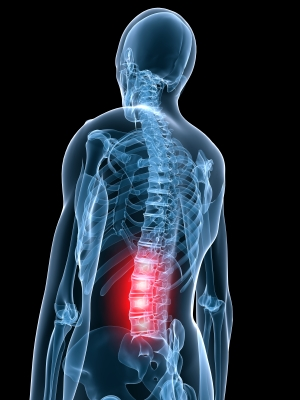
\includegraphics[width=2in]{figures/spinal1.jpg}}{girardgibbs.com}

\column{0.55\textwidth}
\centering
\sig{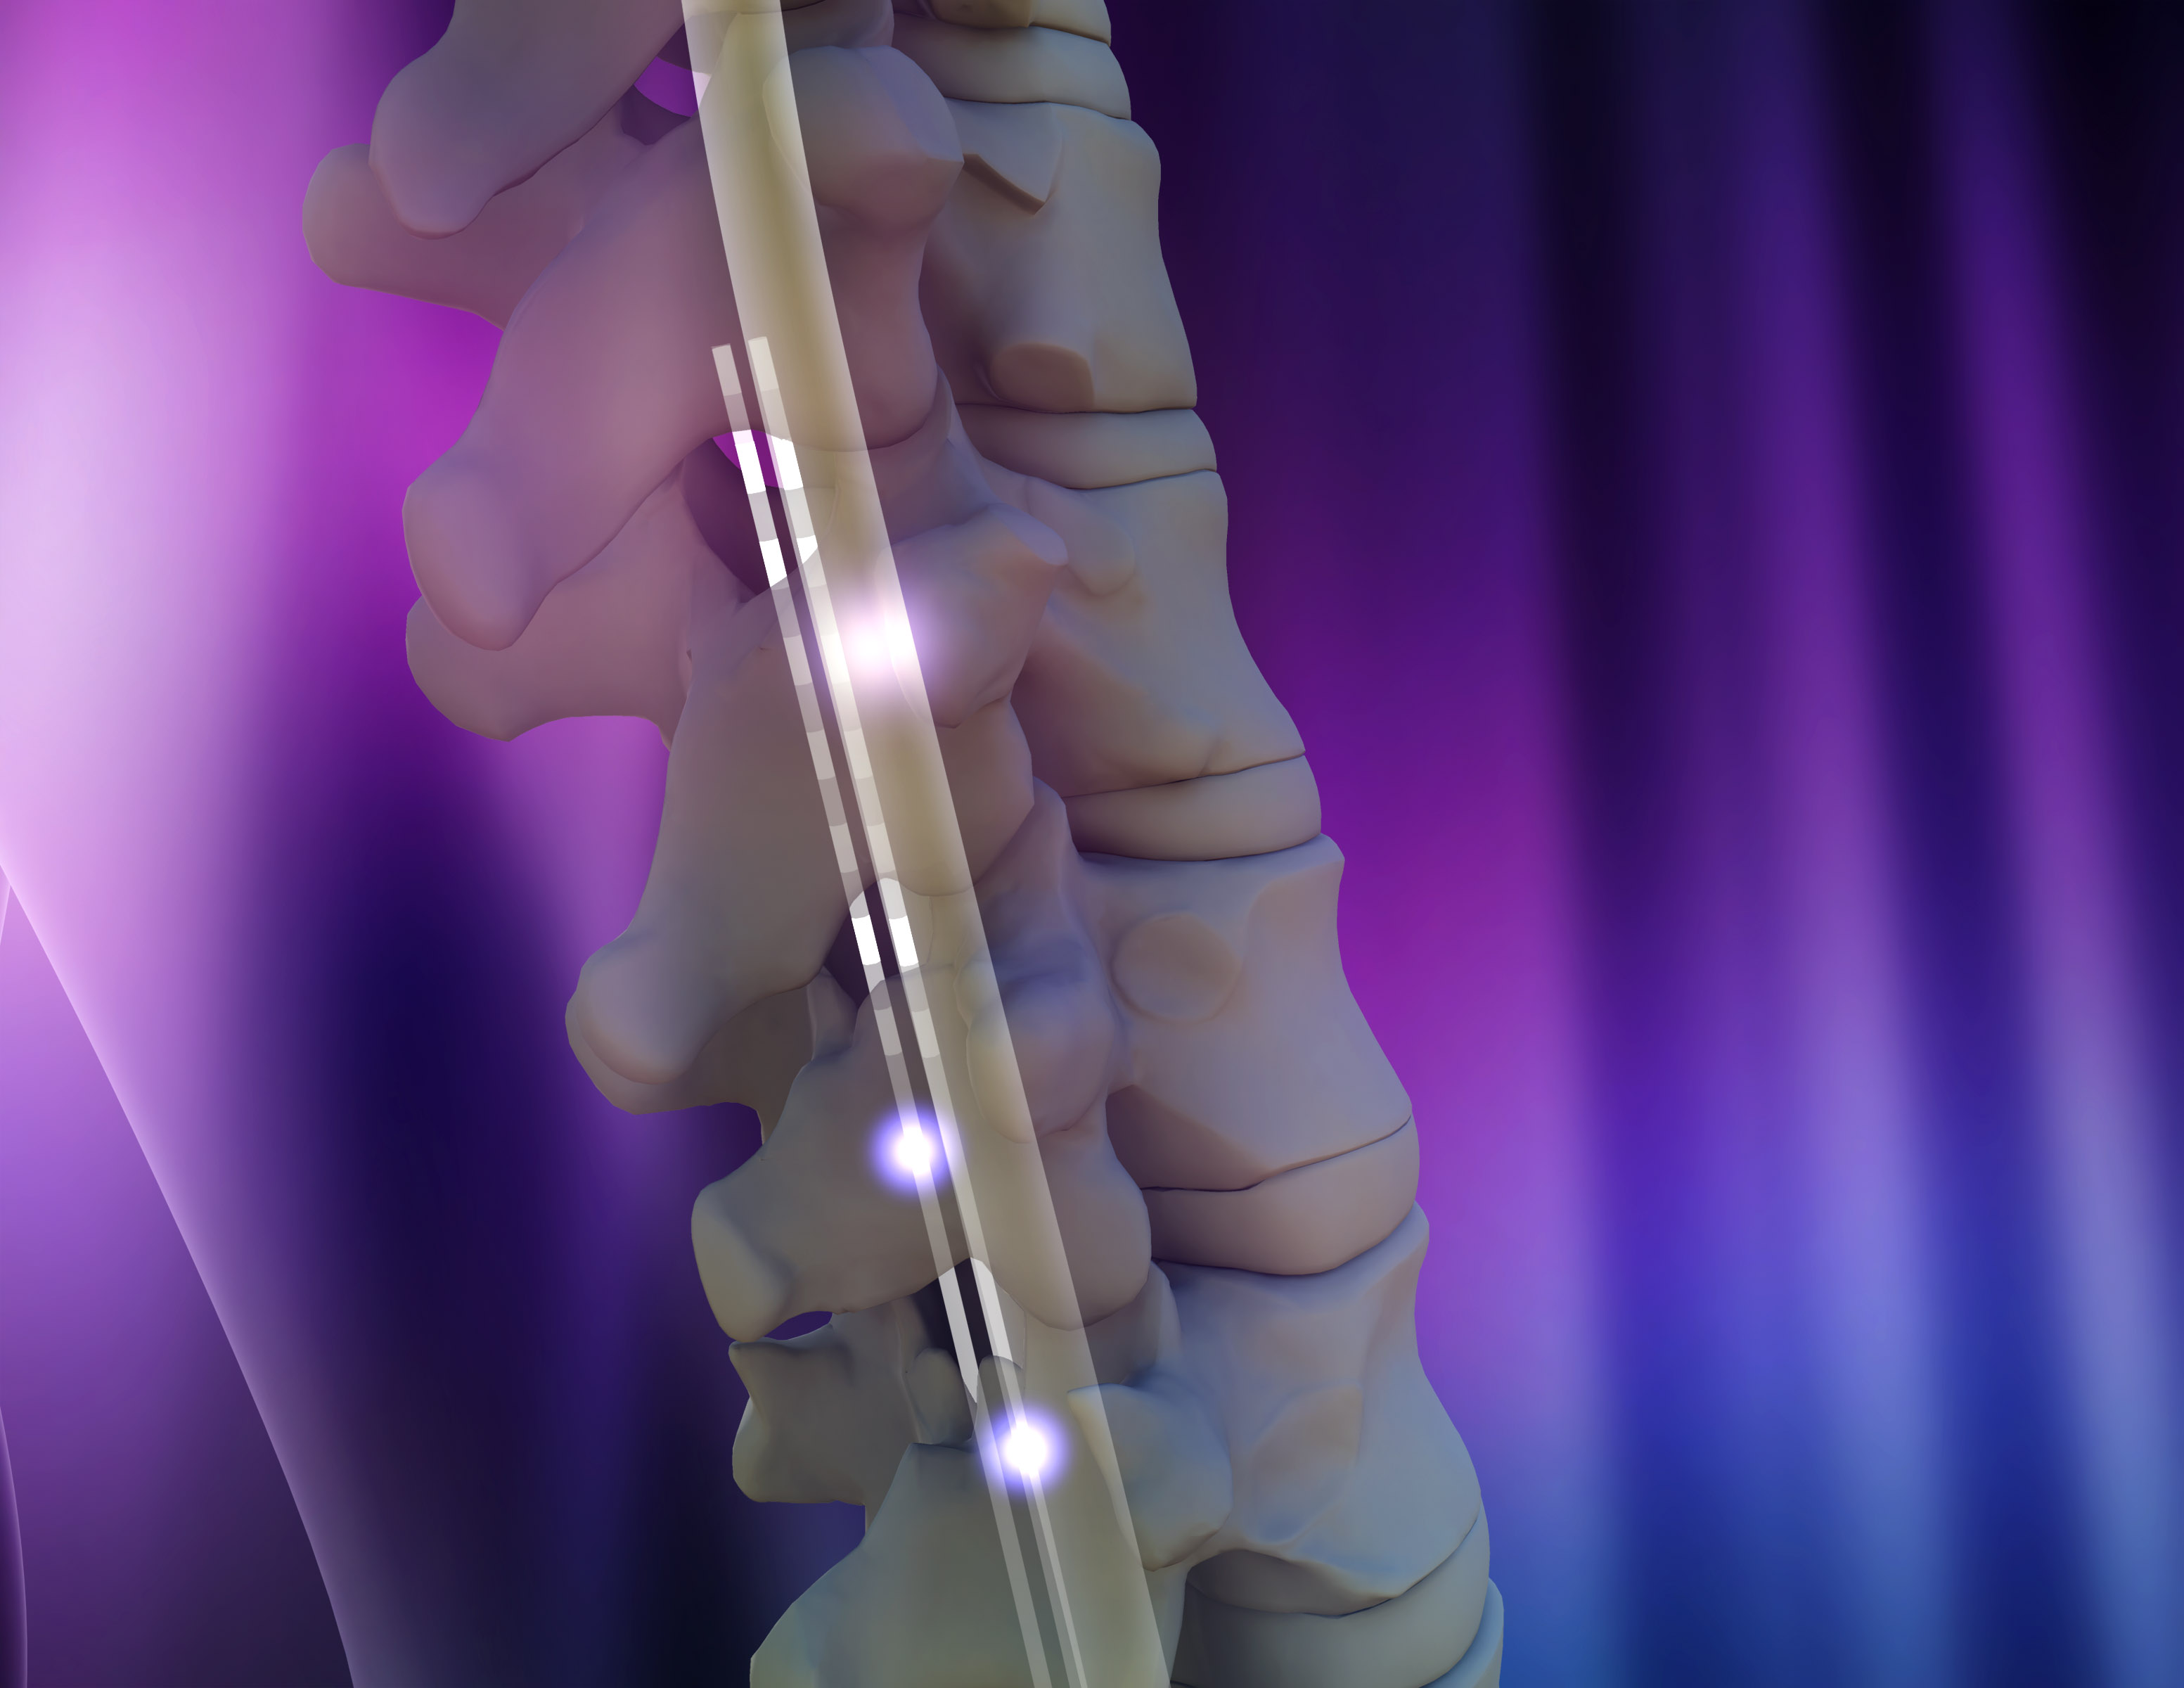
\includegraphics[width=2.45in]{figures/spinal2.jpg}}{sjm.com}
\begin{itemize}
\item Find electrode configurations that maximize muscle activity
\item Bad configurations may cause pain or have negative effects on treatment
\end{itemize}
\end{columns}
\end{frame}

\begin{frame}{Movie recommendation}
\centering
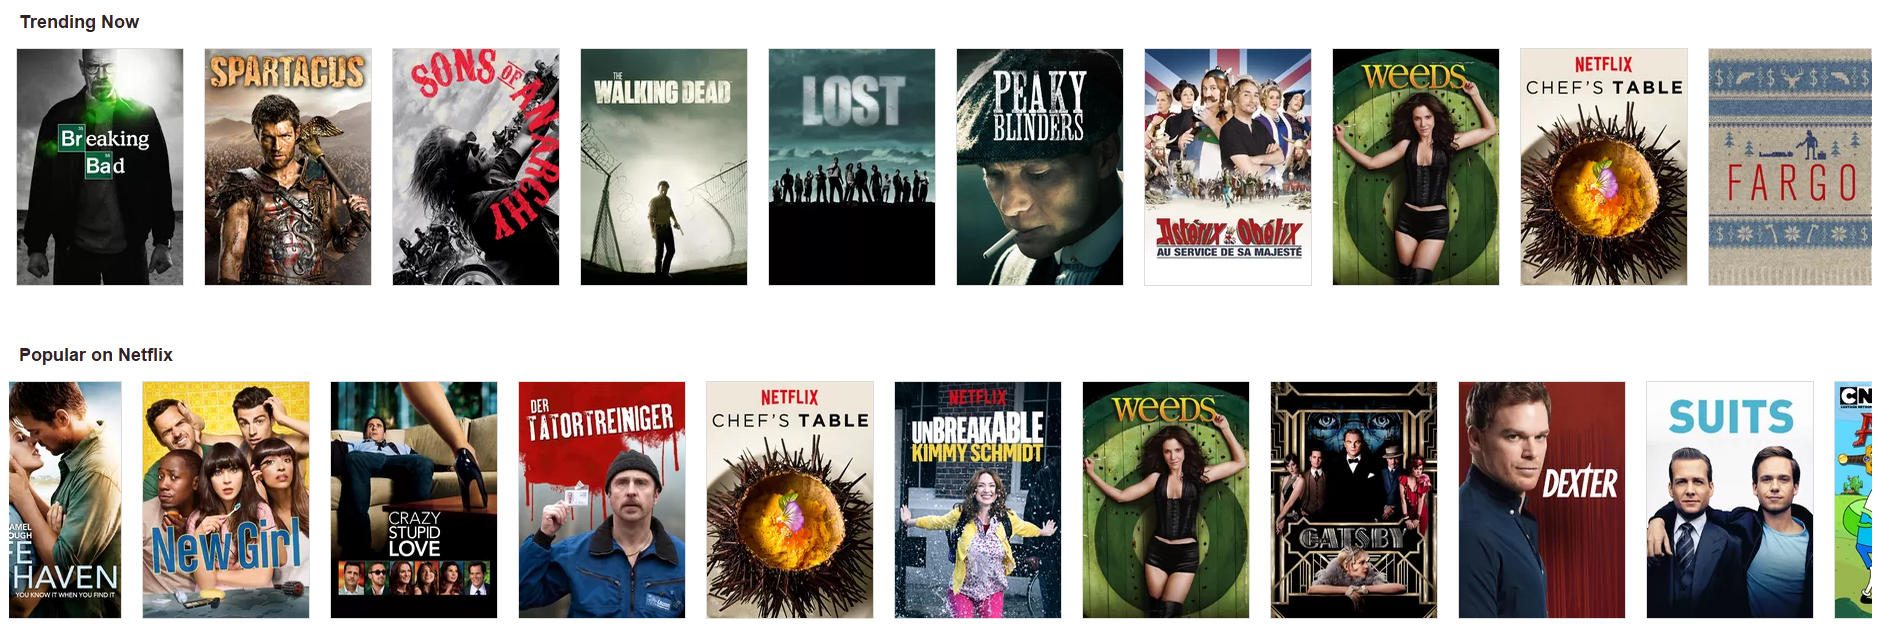
\includegraphics[width=4.5in]{figures/netflix.png}
\vspace{2em}
\begin{itemize}
\item Explore the movie space to discover each user's taste profile
\item Bad recommendations may cause user dissatisfaction
\end{itemize}
\end{frame}

\begin{frame}{Goal}
\centering
\large
Optimize an unknown reward function via sequential sampling\\[1em]
AND\\[1em]
remain ``safe" throughout the process.
\end{frame}

\begin{frame}{Problem statement}

\uncover<1->{
{\large Setup}
\begin{itemize}
\item Finite set $D$
\item Unknown reward function $f : D \to \mathbb{R}$
\item Safety threshold $h \in \mathbb{R}$ ($x$ is called safe, if $f(x) \geq h$)
\item Seed set $S_0$ of safe decisions ($\forall x \in S_0,\ f(x) \geq h$)
\end{itemize}
\vspace{1em}
}

\uncover<2->{
{\large Sequential sampling}
\begin{itemize}
\item For $t = 1, 2, \ldots$
  \begin{itemize}
    \item select $x_t \in D$
    \item observe $f(x_t) + n_t$
  \end{itemize}
\end{itemize}
\vspace{1em}
}

\uncover<3->{
{\large Goal}
\begin{itemize}
\item Locate an optimum $x^* \in \displaystyle\argmax_{x\in D}\left(f(x)\right)$
\item Remain safe: $\forall t \geq 1,\ f(x_t) \geq h$
\end{itemize}
}
\end{frame}

\begin{frame}{Certifying safety}

\uncover<1->{
{\large Assumptions}
\begin{itemize}
\item $d$ is a metric on $D$
\item $f$ is $L$-Lipschitz continuous w.r.t. $d$
\end{itemize}
\vspace{2em}
}

\uncover<2->{
{\large Safety certificate}\\[0.5em]
If we know $f(x)$ for some (safe) $x$, then we can certify as safe any $x'$, such that
\begin{align*}
f(x) - L\,d(x, x') \geq h
\end{align*}
}
\end{frame}

\begin{frame}{Certifying safety}
\centering
\setlength\figurewidth{4.2in}
\setlength\figureheight{2.36in}
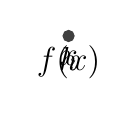
\begin{tikzpicture}

\begin{axis}[%
tick label style={font=\large},
label style={font=\large},
label shift={-4pt},
xlabel shift={-6pt},
legend style={font=\large},
xticklabel shift={2pt},
view={0}{90},
width=\figurewidth,
height=\figureheight,
scale only axis,
xmin=0, xmax=3,
ymin=-4, ymax=4,
xticklabels={,,},
yticklabels={,,},
tickwidth=0cm,
clip=false
]

\addplot [
color=red!40!yellow,
solid,
%only marks,
%mark=square*,
%mark size=3.5pt,
line width=6pt,
forget plot
]
coordinates{
(0.4285,-3.85)(1.5714,-3.85)
};

\addplot [
color=magenta!50!darkgray,
dashed,
line width=1.5pt,
forget plot
]
coordinates{
 (0,-1)(3,-1)
};

\addplot [
color=gray,
solid,
line width=1.2pt,
forget plot
]
coordinates{
 (0,-1.75)(3,3.5)
};

\addplot [
color=gray,
solid,
line width=1.2pt,
forget plot
]
coordinates{
 (0,1.75)(3,-3.5)
};

\addplot [
color=gray,
densely dotted,
line width=1pt,
forget plot
]
coordinates{
 (1,0)(1,-4)
};

\addplot [
color=gray,
densely dotted,
line width=1pt,
forget plot
]
coordinates{
 (0,0)(1,0)
};

\addplot [
mark=*,
color=darkgray,
forget plot
]
coordinates{
 (1,0)
};

\node at (axis cs:1,-4.1) [anchor=north,minimum size=16pt] {\large$x$};
\node at (axis cs:-0.15,0.4) [anchor=north,minimum size=16pt] {\large$f(x)$};
\node at (axis cs:-0.1,-0.6) [anchor=north,minimum size=16pt] {\large$h$};

\end{axis}
\end{tikzpicture}%

\end{frame}

\begin{frame}{Certifying safety}
\centering
\setlength\figurewidth{4.2in}
\setlength\figureheight{2.36in}
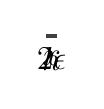
\begin{tikzpicture}

\begin{axis}[%
tick label style={font=\large},
label style={font=\large},
label shift={-4pt},
xlabel shift={-6pt},
legend style={font=\large},
xticklabel shift={2pt},
view={0}{90},
width=\figurewidth,
height=\figureheight,
scale only axis,
xmin=0, xmax=3,
ymin=-4, ymax=4,
xticklabels={,,},
yticklabels={,,},
tickwidth=0cm,
clip=false
]

\addplot [
color=red!40!yellow,
solid,
%only marks,
%mark=square*,
%mark size=3.5pt,
line width=6pt,
forget plot
]
coordinates{
(0.714,-3.85)(1.286,-3.85)
};

\addplot [
color=magenta!50!darkgray,
dashed,
line width=1.5pt,
forget plot
]
coordinates{
 (0,-1)(3,-1)
};

\addplot [
color=gray,
solid,
line width=1.2pt,
forget plot
]
coordinates{
 (0,-2.25)(1,-0.5)
};

\addplot [
color=gray,
solid,
line width=1.2pt,
forget plot
]
coordinates{
 (1,-0.5)(3,-4)
};

\addplot [
color=gray,
solid,
line width=1.2pt,
forget plot
]
coordinates{
 (0,2.25)(1,0.5)
};

\addplot [
color=gray,
solid,
line width=1.2pt,
forget plot
]
coordinates{
 (1,0.5)(3,4)
};

\addplot [
color=gray,
densely dotted,
line width=1pt,
forget plot
]
coordinates{
 (1,0)(1,-4)
};

\addplot [
color=gray,
densely dotted,
line width=1pt,
forget plot
]
coordinates{
 (0,-0.5)(1,-0.5)
};

\addplot [
color=gray,
densely dotted,
line width=1pt,
forget plot
]
coordinates{
 (0,0.5)(1,0.5)
};

\addplot [
mark=-,
color=darkgray,
line width=1.2pt,
forget plot
]
coordinates{
 (1,-0.5)(1,0.5)
};

\node at (axis cs:1,-4.1) [anchor=north,minimum size=16pt] {\large$x$};
\node at (axis cs:-0.1,0.4) [anchor=north,minimum size=16pt] {\large$2\epsilon$};
\node at (axis cs:-0.1,-0.6) [anchor=north,minimum size=16pt] {\large$h$};

\end{axis}
\end{tikzpicture}%

\end{frame}

\begin{frame}{Reachability}

\uncover<1->{
{\large One-step reachability operator}
\begin{align*}
\Reps(S) := S \cup \left\{x' \in D \mid \exists x \in S,\ f(x) - \epsilon - L\,d(x, x') \geq h\right\}
\end{align*}
\vspace{1em}
}

\uncover<2->{
{\large $n$-step reachability operator}
\begin{align*}
\Reps^n(S) := \underbrace{\Reps(\Reps\ldots(\Reps}_{n\ \mathrm{times}}(S))\ldots)
\end{align*}
\vspace{1em}
}

\uncover<3->{
{\large $\epsilon$-reachable set from $S$}
\begin{align*}
\Rbeps(S) := \displaystyle\lim_{n \to \infty} \Reps^n(S)
\end{align*}
}
\end{frame}

\begin{frame}{Reconsidering optimization}
\begin{itemize}
\item<1-> No algorithm that is $\epsilon$-uncertain about $f$ can certify any $x \in D \setminus \Rbeps(S_0)$ as safe
\vspace{2em}
\item<2-> Goal of finding $f^* = \max_{x \in D}\left(f(x)\right)$ is unrealistic
\vspace{2em}
\item<3-> Instead, aim for the $\epsilon$-reachable maximum
  \begin{align*}
    f_{\epsilon}^* = \max_{x \in \Rbeps(S_0)}\left(f(x)\right)
  \end{align*}
\end{itemize}
\end{frame}

\begin{frame}{Estimating $f$}
\begin{itemize}
\item<1-> To certify safety, we need to estimate $f$
\vspace{2em}
\item<2-> Additional assumption: $f$ has bounded norm in the RKHS associated with some kernel $k$ defined on $D$
\vspace{2em}
\item<3-> Then, we can model $f$ as a Gaussian process and obtain confidence estimates
\end{itemize}
\end{frame}

\begin{frame}{Estimating $f$}
\centering
\setlength\figurewidth{4.2in}
\setlength\figureheight{2.36in}
% This file was created by matlab2tikz v0.2.3.
% Copyright (c) 2008--2012, Nico Schlömer <nico.schloemer@gmail.com>
% All rights reserved.
% 
% 
%
\definecolor{locol}{rgb}{0.26, 0.45, 0.65}

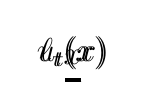
\begin{tikzpicture}

\begin{axis}[%
tick label style={font=\large},
label style={font=\large},
label shift={-4pt},
xlabel shift={-6pt},
legend style={font=\large},
view={0}{90},
width=\figurewidth,
height=\figureheight,
scale only axis,
xmin=0, xmax=2,
ymin=-2, ymax=4,
xticklabels={,,},
yticklabels={,,},
tickwidth=0cm,
clip=false
]

\addplot [fill=olive!20!lightgray,draw=none,forget plot] coordinates{ (0,3.58482942463052)(0.01,3.60004798891101)(0.02,3.61522857444221)(0.03,3.63033189586352)(0.04,3.64531565363331)(0.05,3.66013442184805)(0.06,3.67473953961915)(0.07,3.68907900710597)(0.08,3.70309738743443)(0.09,3.71673571587552)(0.1,3.72993141781888)(0.11,3.742618237255)(0.12,3.75472617767874)(0.13,3.76618145754966)(0.14,3.77690648269497)(0.15,3.78681983832409)(0.16,3.79583630364506)(0.17,3.80386689244192)(0.18,3.81081892339735)(0.19,3.81659612444073)(0.2,3.82109877598645)(0.21,3.82422389862386)(0.22,3.82586549166252)(0.23,3.82591482996835)(0.24,3.82426082780994)(0.25,3.82079048005803)(0.26,3.81538939316725)(0.27,3.80794242109654)(0.28,3.79833442495176)(0.29,3.78645118004131)(0.3,3.77218046079061)(0.31,3.7554133434235)(0.32,3.73604577980269)(0.33,3.71398051537493)(0.34,3.68912945302201)(0.35,3.66141660795913)(0.36,3.63078186508568)(0.37,3.59718585332289)(0.38,3.56061641480533)(0.39,3.52109740977021)(0.4,3.47870102745279)(0.41,3.43356548123227)(0.42,3.3859211324836)(0.43,3.33612996677294)(0.44,3.28474615977828)(0.45,3.23260879787809)(0.46,3.18097820535255)(0.47,3.13171088766885)(0.48,3.08739598582499)(0.49,3.05119669234731)(0.5,3.0259838611258)(0.51,3.01284772838793)(0.52,3.01029666091057)(0.53,3.01514563996159)(0.54,3.02402797128164)(0.55,3.0342360054454)(0.56,3.04384617507831)(0.57,3.0515590388948)(0.58,3.05651103425065)(0.59,3.05813122154211)(0.6,3.05604507798808)(0.61,3.05001223160369)(0.62,3.0398862161563)(0.63,3.02558807820813)(0.64,3.00708869268196)(0.65,2.9843966280902)(0.66,2.95754962228728)(0.67,2.92660846538683)(0.68,2.89165253089039)(0.69,2.85277646735342)(0.7,2.81008773105625)(0.71,2.76370474622489)(0.72,2.71375554757698)(0.73,2.66037680479363)(0.74,2.6037131586945)(0.75,2.54391681983164)(0.76,2.48114739535772)(0.77,2.41557192163831)(0.78,2.34736508976863)(0.79,2.27670966017863)(0.8,2.20379707201033)(0.81,2.12882826416686)(0.82,2.05201473942949)(0.83,1.97357992300915)(0.84,1.89376089562466)(0.85,1.81281062378027)(0.86,1.73100087447615)(0.87,1.64862610128955)(0.88,1.56600874517876)(0.89,1.48350664197121)(0.9,1.40152362731363)(0.91,1.32052507105654)(0.92,1.24106109190918)(0.93,1.16380175577295)(0.94,1.0895906611355)(0.95,1.01952516621653)(0.96,0.955069311764951)(0.97,0.898186752650931)(0.98,0.851416932475347)(0.99,0.817685171628646)(1,0.799565107889029)(1.01,0.798121861452096)(1.02,0.812289633856214)(1.03,0.8394941968923)(1.04,0.876809815423523)(1.05,0.921696894661266)(1.06,0.972191980008956)(1.07,1.026831670377)(1.08,1.08451977451554)(1.09,1.1444144761036)(1.1,1.2058481943895)(1.11,1.26827408639539)(1.12,1.33123093587662)(1.13,1.39432002549962)(1.14,1.45718968863576)(1.15,1.51952478969417)(1.16,1.58103940072838)(1.17,1.6414715831874)(1.18,1.70057958243273)(1.19,1.7581389911792)(1.2,1.81394059435028)(1.21,1.86778870745259)(1.22,1.91949988503488)(1.23,1.96890191826689)(1.24,2.01583306927621)(1.25,2.06014150971716)(1.26,2.10168494539283)(1.27,2.14033041980383)(1.28,2.17595429881624)(1.29,2.20844244746681)(1.3,2.23769061939598)(1.31,2.26360509077436)(1.32,2.28610358546564)(1.33,2.30511655881966)(1.34,2.32058893735021)(1.35,2.33248245603253)(1.36,2.34077880280757)(1.37,2.34548388554397)(1.38,2.34663370439796)(1.39,2.34430258329642)(1.4,2.33861495813319)(1.41,2.32976265446075)(1.42,2.31803080653477)(1.43,2.30383755357099)(1.44,2.28779567363942)(1.45,2.27080806509891)(1.46,2.25421017454742)(1.47,2.2399573025432)(1.48,2.23078349147602)(1.49,2.23007528043064)(1.5,2.24102962233239)(1.51,2.2651406710595)(1.52,2.30131039476205)(1.53,2.34665072790035)(1.54,2.3979733507103)(1.55,2.45265743944081)(1.56,2.50880945592376)(1.57,2.56512775906107)(1.58,2.62072860112149)(1.59,2.67501062618579)(1.6,2.72756287250157)(1.61,2.7781048370449)(1.62,2.82644754667784)(1.63,2.87246790701773)(1.64,2.91609141311241)(1.65,2.95728018449664)(1.66,2.99602445277282)(1.67,3.03233633720696)(1.68,3.06624517275588)(1.69,3.09779391742564)(1.7,3.12703632874307)(1.71,3.15403470183875)(1.72,3.17885802752753)(1.73,3.20158047176855)(1.74,3.22228010642895)(1.75,3.24103784054218)(1.76,3.25793651447589)(1.77,3.27306012864814)(1.78,3.28649318497019)(1.79,3.2983201239044)(1.8,3.30862484347432)(1.81,3.3174902891288)(1.82,3.32499810530132)(1.83,3.33122834099536)(1.84,3.3362592028899)(1.85,3.34016685038152)(1.86,3.34302522772289)(1.87,3.34490592902509)(1.88,3.34587809239502)(1.89,3.34600831990287)(1.9,3.34536062043468)(1.91,3.34399637279505)(1.92,3.34197430669431)(1.93,3.33935049949039)(1.94,3.33617838676422)(1.95,3.33250878499287)(1.96,3.32838992475032)(1.97,3.32386749301519)(1.98,3.31898468329879)(1.99,3.31378225242948)(2,3.30829858293919)(2,-0.444829374793357)(1.99,-0.421098651071882)(1.98,-0.396446336163294)(1.97,-0.370845345516832)(1.96,-0.344268698795504)(1.95,-0.316689632748587)(1.94,-0.288081726215209)(1.93,-0.25841903808521)(1.92,-0.227676259077674)(1.91,-0.195828878232804)(1.9,-0.162853365049562)(1.89,-0.128727368240436)(1.88,-0.0934299321168721)(1.87,-0.0569417316656629)(1.86,-0.0192453274299609)(1.85,0.0196745586284737)(1.84,0.0598307450330455)(1.83,0.101233269114178)(1.82,0.143889040279859)(1.81,0.187801466606901)(1.8,0.23297005291475)(1.79,0.279389968201148)(1.78,0.327051579935454)(1.77,0.375939952180139)(1.76,0.426034303786354)(1.75,0.477307421903277)(1.74,0.529725024634428)(1.73,0.583245064695554)(1.72,0.637816963125363)(1.71,0.693380758098698)(1.7,0.749866148131158)(1.69,0.807191400594332)(1.68,0.865262084174702)(1.67,0.923969565669119)(1.66,0.983189184093607)(1.65,1.04277797331801)(1.64,1.10257173990012)(1.63,1.16238120155058)(1.62,1.22198673039036)(1.61,1.28113098443977)(1.6,1.33950828377602)(1.59,1.39674888254904)(1.58,1.45239512476716)(1.57,1.50586459578307)(1.56,1.55639257115558)(1.55,1.60294274080495)(1.54,1.64407480352181)(1.53,1.67777397387581)(1.52,1.70131956298155)(1.51,1.71144924430573)(1.5,1.70523183993032)(1.49,1.68156264538277)(1.48,1.64196899135767)(1.47,1.58971783498313)(1.46,1.52829738913243)(1.45,1.46057039095885)(1.44,1.38864376767554)(1.43,1.31402394188051)(1.42,1.23780101275596)(1.41,1.1607884731007)(1.4,1.08361635276817)(1.39,1.00679085020874)(1.38,0.930732327842318)(1.37,0.855799800322401)(1.36,0.782307022733014)(1.35,0.710533304055332)(1.34,0.640730954228341)(1.33,0.573130539780742)(1.32,0.507944680783682)(1.31,0.445370852532745)(1.3,0.385593488936256)(1.29,0.328785580005791)(1.28,0.275109888906981)(1.27,0.224719870300608)(1.26,0.177760342439145)(1.25,0.134367945276811)(1.24,0.094671402268187)(1.23,0.0587915923031793)(1.22,0.0268414287544383)(1.21,-0.00107446635636632)(1.2,-0.0248603146781139)(1.19,-0.0444299934333956)(1.18,-0.0597081549437549)(1.17,-0.0706317224008323)(1.16,-0.0771518600220896)(1.15,-0.079236559279762)(1.14,-0.0768740486083972)(1.13,-0.0700773350515127)(1.12,-0.0588903442762789)(1.11,-0.0433963757642554)(1.1,-0.0237299907984804)(1.09,-9.40942984856141e-05)(1.08,0.0272150070885241)(1.07,0.0577702328946769)(1.06,0.0909576019586149)(1.05,0.125893055316186)(1.04,0.161306130482944)(1.03,0.195403125446262)(1.02,0.225786465151679)(1.01,0.249639542185894)(1,0.264458529378529)(0.99,0.26920285236244)(0.98,0.264913763770812)(0.97,0.254095681204893)(0.96,0.239565626824373)(0.95,0.223721326871451)(0.94,0.208356283085153)(0.93,0.194740318290634)(0.92,0.183756324482167)(0.91,0.176016500654449)(0.9,0.171945442125653)(0.89,0.171836179811568)(0.88,0.175887465025862)(0.87,0.184228740738409)(0.86,0.196937137231983)(0.85,0.214049274806336)(0.84,0.23556963487419)(0.83,0.261476617420922)(0.82,0.291727002053005)(0.81,0.326259279554266)(0.8,0.364996162981932)(0.79,0.407846486369675)(0.78,0.454706633488184)(0.77,0.505461595674604)(0.76,0.55998572834969)(0.75,0.618143255391288)(0.74,0.679788555740815)(0.73,0.744766255290415)(0.72,0.812911137667727)(0.71,0.884047878763875)(0.7,0.957990600596524)(0.69,1.0345422291118)(0.68,1.11349362620844)(0.67,1.19462244634792)(0.66,1.27769163916542)(0.65,1.36244747611301)(0.64,1.4486169126074)(0.63,1.53590399298656)(0.62,1.62398483960066)(0.61,1.71250049851602)(0.6,1.80104647262306)(0.59,1.88915704018206)(0.58,1.97628124047184)(0.57,2.06174542720433)(0.56,2.14469426911443)(0.55,2.22399833130533)(0.54,2.29811518586665)(0.53,2.36490617240151)(0.52,2.42148216079223)(0.51,2.46433509334006)(0.5,2.49018607872373)(0.49,2.49750526559355)(0.48,2.48740515404448)(0.47,2.46283413364432)(0.46,2.42707965816406)(0.45,2.38289409924225)(0.44,2.3323292750101)(0.43,2.27686680349494)(0.42,2.21758765612926)(0.41,2.15530373759552)(0.4,2.09064643872724)(0.39,2.02412355716508)(0.38,1.95615559851786)(0.37,1.88709914785574)(0.36,1.81726219187339)(0.35,1.7469143967805)(0.34,1.6762941843428)(0.33,1.60561374383708)(0.32,1.53506269122152)(0.31,1.46481082659219)(0.3,1.3950102801787)(0.29,1.32579723630126)(0.28,1.2572933605496)(0.27,1.18960701402354)(0.26,1.12283431137273)(0.25,1.05706006141912)(0.24,0.992358617120402)(0.23,0.928794653500352)(0.22,0.866423886627792)(0.21,0.805293742920604)(0.2,0.745443985426882)(0.19,0.686907301918829)(0.18,0.629709858375887)(0.17,0.573871820560741)(0.16,0.519407845788207)(0.15,0.466327546571051)(0.14,0.414635927542119)(0.13,0.364333796858902)(0.12,0.315418153166848)(0.11,0.267882549111694)(0.1,0.221717432334636)(0.09,0.176910464847661)(0.08,0.133446821662446)(0.07,0.091309469530374)(0.06,0.0504794266397142)(0.05,0.010936004106592)(0.04,-0.0273429699125187)(0.03,-0.0643809426684996)(0.02,-0.100202445019883)(0.01,-0.13483291459035)(0,-0.168298533102028)};

\addplot [
color=olive!70!black,
solid,
line width=2.0pt,
forget plot
]
coordinates{
  (0,1.70826544576424)(0.01,1.73260753716033)(0.02,1.75751306471116)(0.03,1.78297547659751)(0.04,1.8089863418604)(0.05,1.83553521297732)(0.06,1.86260948312943)(0.07,1.89019423831817)(0.08,1.91827210454844)(0.09,1.94682309036159)(0.1,1.97582442507676)(0.11,2.00525039318335)(0.12,2.0350721654228)(0.13,2.06525762720428)(0.14,2.09577120511855)(0.15,2.12657369244757)(0.16,2.15762207471663)(0.17,2.18886935650133)(0.18,2.22026439088662)(0.19,2.25175171317978)(0.2,2.28327138070667)(0.21,2.31475882077223)(0.22,2.34614468914516)(0.23,2.37735474173435)(0.24,2.40830972246517)(0.25,2.43892527073858)(0.26,2.46911185226999)(0.27,2.49877471756004)(0.28,2.52781389275068)(0.29,2.55612420817129)(0.3,2.58359537048465)(0.31,2.61011208500784)(0.32,2.6355542355121)(0.33,2.659797129606)(0.34,2.6827118186824)(0.35,2.70416550236982)(0.36,2.72402202847953)(0.37,2.74214250058932)(0.38,2.75838600666159)(0.39,2.77261048346765)(0.4,2.78467373309002)(0.41,2.7944346094139)(0.42,2.80175439430643)(0.43,2.80649838513394)(0.44,2.80853771739419)(0.45,2.80775144856017)(0.46,2.8040289317583)(0.47,2.79727251065658)(0.48,2.78740056993473)(0.49,2.77435097897043)(0.5,2.75808496992476)(0.51,2.738591410864)(0.52,2.7158894108514)(0.53,2.69002590618155)(0.54,2.66107157857415)(0.55,2.62911716837536)(0.56,2.59427022209637)(0.57,2.55665223304956)(0.58,2.51639613736124)(0.59,2.47364413086208)(0.6,2.42854577530557)(0.61,2.38125636505986)(0.62,2.33193552787848)(0.63,2.28074603559734)(0.64,2.22785280264468)(0.65,2.1734220521016)(0.66,2.11762063072635)(0.67,2.06061545586737)(0.68,2.00257307854941)(0.69,1.94365934823261)(0.7,1.88403916582639)(0.71,1.82387631249438)(0.72,1.76333334262236)(0.73,1.70257153004202)(0.74,1.64175085721766)(0.75,1.58103003761146)(0.76,1.5205665618537)(0.77,1.46051675865646)(0.78,1.40103586162841)(0.79,1.34227807327415)(0.8,1.28439661749613)(0.81,1.22754377186056)(0.82,1.17187087074125)(0.83,1.11752827021504)(0.84,1.06466526524942)(0.85,1.01342994929331)(0.86,0.963969005854064)(0.87,0.916427421013977)(0.88,0.87094810510231)(0.89,0.82767141089139)(0.9,0.786734534719644)(0.91,0.748270785855492)(0.92,0.712408708195676)(0.93,0.679271037031793)(0.94,0.648973472110324)(0.95,0.621623246543991)(0.96,0.597317469294662)(0.97,0.576141216927912)(0.98,0.55816534812308)(0.99,0.543444011995543)(1,0.532011818633779)(1.01,0.523880701818995)(1.02,0.519038049503947)(1.03,0.517448661169281)(1.04,0.519057972953233)(1.05,0.523794974988726)(1.06,0.531574790983785)(1.07,0.542300951635837)(1.08,0.555867390802034)(1.09,0.572160190902558)(1.1,0.591059101795511)(1.11,0.612438855315566)(1.12,0.63617029580017)(1.13,0.662121345224055)(1.14,0.690157820013684)(1.15,0.720144115207205)(1.16,0.751943770353143)(1.17,0.785419930393282)(1.18,0.820435713744487)(1.19,0.856854498872902)(1.2,0.894540139836085)(1.21,0.933357120548111)(1.22,0.973170656894659)(1.23,1.01384675528503)(1.24,1.0552522357722)(1.25,1.09725472749698)(1.26,1.13972264391599)(1.27,1.18252514505222)(1.28,1.22553209386161)(1.29,1.2686140137363)(1.3,1.31164205416612)(1.31,1.35448797165355)(1.32,1.39702413312466)(1.33,1.4391235493002)(1.34,1.48065994578927)(1.35,1.52150788004393)(1.36,1.56154291277029)(1.37,1.60064184293319)(1.38,1.63868301612014)(1.39,1.67554671675258)(1.4,1.71111565545068)(1.41,1.74527556378072)(1.42,1.77791590964536)(1.43,1.80893074772575)(1.44,1.83821972065748)(1.45,1.86568922802888)(1.46,1.89125378183992)(1.47,1.91483756876317)(1.48,1.93637624141684)(1.49,1.9558189629067)(1.5,1.97313073113136)(1.51,1.98829495768261)(1.52,2.0013149788718)(1.53,2.01221235088808)(1.54,2.02102407711605)(1.55,2.02780009012288)(1.56,2.03260101353967)(1.57,2.03549617742207)(1.58,2.03656186294433)(1.59,2.03587975436742)(1.6,2.0335355781388)(1.61,2.02961791074233)(1.62,2.0242171385341)(1.63,2.01742455428415)(1.64,2.00933157650626)(1.65,2.00002907890732)(1.66,1.98960681843321)(1.67,1.97815295143804)(1.68,1.96575362846529)(1.69,1.95249265900999)(1.7,1.93845123843711)(1.71,1.92370772996873)(1.72,1.90833749532644)(1.73,1.89241276823205)(1.74,1.87600256553169)(1.75,1.85917263122273)(1.76,1.84198540913112)(1.77,1.82450004041414)(1.78,1.80677238245282)(1.79,1.78885504605277)(1.8,1.77079744819454)(1.81,1.75264587786785)(1.82,1.73444357279059)(1.83,1.71623080505477)(1.84,1.69804497396147)(1.85,1.67992070450499)(1.86,1.66188995014647)(1.87,1.64398209867971)(1.88,1.62622408013907)(1.89,1.60864047583122)(1.9,1.59125362769256)(1.91,1.57408374728112)(1.92,1.55714902380832)(1.93,1.54046573070259)(1.94,1.52404833027451)(1.95,1.50790957612214)(1.96,1.49206061297741)(1.97,1.47651107374918)(1.98,1.46126917356775)(1.99,1.4463418006788)(2,1.43173460407292) 
};

\addplot [
color=gray,
densely dotted,
line width=1pt,
forget plot
]
coordinates{
 (1.23,-2)(1.23,-0)
};

\addplot [
color=black,
solid,
line width=1.5pt,
mark=-,
mark size=3pt,
forget plot
]
coordinates{
 (1.23,0.0268)(1.23,1.9195)
};

\node at (axis cs:1.12,1.77) [anchor=south,minimum size=16pt] {\large$u_t(x)$};
\node at (axis cs:1.35,-0.3) [anchor=south,minimum size=16pt] {\large$\ell_t(x)$};
\node at (axis cs:1.23,-2.6) [anchor=south,minimum size=16pt] {\large$x$};

\end{axis}
\end{tikzpicture}%


Width of confidence interval $w_t(x) := u_t(x) - \ell_t(x)$
\end{frame}

\begin{frame}{Algorithm components}

\uncover<1->{
{\large Safe set}
\begin{align*}
S_t := \bigcup_{x \in S_{t-1}}\bigsetdef{x' \in D}{\ell_t(x) - L\,d(x, x') \geq h}
\end{align*}
\vspace{0.5em}
}

\uncover<2->{
{\large Potential maximizers}
\begin{align*}
M_t := \bigsetdef{x\in S_t}{u_t(x)\geq \max_{x'\in S_t} \ell_t(x')}
\end{align*}
\vspace{0.5em}
}

\uncover<3->{
{\large Potential expanders}
\begin{align*}
G_t := \bigsetdef{x\in S_t}{g_t(x)>0}
\end{align*}
}
\uncover<4->{
Function $g_t(x)$ quantifies the best-case ``certification potential" of $x$:
\begin{align*}
g_t(x) := \Big|\bigsetdef{x' \in D \setminus S_t}{u_t(x) - L\,d(x, x') \geq h}\Big|
\end{align*}
}
\end{frame}

\definecolor{c1}{RGB}{255,255,255}
\definecolor{c2}{RGB}{27,161,226}
\definecolor{c6}{RGB}{140,191,38}
\definecolor{c4}{RGB}{240,150,9}
\definecolor{c5}{RGB}{240,230,60}
\definecolor{c3}{RGB}{230,113,184}
\definecolor{cwhite}{RGB}{255,255,255}

\begin{frame}{The SafeOpt algorithm}
\begin{algorithmic}
  \REQUIRE sample set $D$, kernel $k$, Lipschitz constant $L$, seed set $S_0$, safe threshold $h$
  %\ENSURE predicted super- and sublevel sets
  \STATE
  \uncover<1->{
  \CFOR{cwhite}{$t = 1,2,\ldots$}
  }
    \uncover<2->{
      \CLET{cwhite}{$S_t$}{$\bigcup_{x \in S_{t-1}}\bigsetdef{x' \in D}{\ell_t(x) - L\,d(x, x') \geq h}$}
      \CLET{cwhite}{$M_t$}{$\bigsetdef{x\in S_t}{u_t(x)\geq \max_{x'\in S_t} \ell_t(x')}$}
      \CLET{cwhite}{$G_t$}{$\bigsetdef{x\in S_t}{g_t(x)>0}$}
    }
    \uncover<3->{
      \CLET{cwhite}{$\*x_t$}{$\argmax_{x \in G_t \cup M_t}(w_t(x))$}
      \CLET{cwhite}{$y_t$}{$f(x_t) + n_t$}
    }
    \uncover<4->{
      \CSTATE{cwhite}Update GP estimates
    }
  \uncover<1->{
    \CENDFOR{cwhite}
  }
\end{algorithmic}
\end{frame}

\begin{frame}{1-D example run}
\centering
\setlength\figurewidth{5in}
\setlength\figureheight{2.81in}
\begin{tikzpicture}

\begin{axis}[
tick label style={font=\small},
label style={font=\small},
width=\figurewidth,
height=\figureheight,
xmin=0, xmax=5,
ymin=-4, ymax=2.5,
xticklabels={,,},
yticklabels={,,},
ylabel near ticks,
ylabel shift=-5pt,
major tick length=0pt,
legend cell align=left]

\addplot [
  magenta!50!darkgray,
  line width=1.5pt,
  dashed
]
coordinates{
  (0,-1.17514504)(10,-1.17514504)
};

\addplot[
  gray,
  solid,
  line width=1.5pt,
  samples=30,domain=0:10
]
coordinates{
(0.0,1.06438836926)(0.01,1.09776240042)(0.02,1.12526472291)(0.03,1.14672225178)(0.04,1.16201468957)(0.05,1.1710782945)(0.06,1.17390921713)(0.07,1.17056599097)(0.08,1.1611707436)(0.09,1.14590904219)(0.1,1.12502962659)(0.11,1.09884164521)(0.12,1.0677111579)(0.13,1.032055952)(0.14,0.992339793004)(0.15,0.94906384331)(0.16,0.902758488534)(0.17,0.853972741399)(0.18,0.803263870082)(0.19,0.751184645502)(0.2,0.698273450128)(0.21,0.645039898372)(0.22,0.591955686888)(0.23,0.539442293818)(0.24,0.487859462663)(0.25,0.437500374336)(0.26,0.388580867093)(0.27,0.341236525353)(0.28,0.295520196051)(0.29,0.25139968997)(0.3,0.208761678317)(0.31,0.167415606923)(0.32,0.12710066981)(0.33,0.0874953372339)(0.34,0.0482293956499)(0.35,0.00889560111511)(0.36,-0.0309337878064)(0.37,-0.0716927281696)(0.38,-0.113804700484)(0.39,-0.157666804679)(0.4,-0.203633823659)(0.41,-0.252004675914)(0.42,-0.303008401997)(0.43,-0.356794038868)(0.44,-0.413422197932)(0.45,-0.47285816572)(0.46,-0.534970434593)(0.47,-0.599530588846)(0.48,-0.66621615681)(0.49,-0.734617383665)(0.5,-0.804246456308)(0.51,-0.874549240095)(0.52,-0.944919062491)(0.53,-1.01471253778)(0.54,-1.08326629177)(0.55,-1.14991492804)(0.56,-1.2140077833)(0.57,-1.27492716377)(0.58,-1.33210305797)(0.59,-1.38502912784)(0.6,-1.4332732043)(0.61,-1.47648961122)(0.62,-1.51442526495)(0.63,-1.54692342234)(0.64,-1.57392660895)(0.65,-1.59547442504)(0.66,-1.61169928023)(0.67,-1.6228195426)(0.68,-1.62913011984)(0.69,-1.63099187575)(0.7,-1.62881835326)(0.71,-1.6230628965)(0.72,-1.61420355776)(0.73,-1.60272996737)(0.74,-1.58912896628)(0.75,-1.57387175608)(0.76,-1.5574024602)(0.77,-1.54012785236)(0.78,-1.52240917906)(0.79,-1.50455544093)(0.8,-1.48681914738)(0.81,-1.46939367377)(0.82,-1.45241251554)(0.83,-1.43595072612)(0.84,-1.42002684563)(0.85,-1.40460723395)(0.86,-1.38961041432)(0.87,-1.37491301189)(0.88,-1.36035501344)(0.89,-1.34574596793)(0.9,-1.3308714156)(0.91,-1.31549712601)(0.92,-1.29937508757)(0.93,-1.28224801142)(0.94,-1.26385281079)(0.95,-1.24392369855)(0.96,-1.2221951493)(0.97,-1.19840355766)(0.98,-1.17228940105)(0.99,-1.14359851247)(1.0,-1.11208317095)(1.01,-1.0775037506)(1.02,-1.0396305288)(1.03,-0.998245681666)(1.04,-0.953145263234)(1.05,-0.904142379648)(1.06,-0.851071122614)(1.07,-0.793790036612)(1.08,-0.732187277012)(1.09,-0.666184711006)(1.1,-0.595743906277)(1.11,-0.520870684692)(1.12,-0.441621135525)(1.13,-0.358105832774)(1.14,-0.270494194422)(1.15,-0.179018262603)(1.16,-0.0839754321483)(1.17,0.0142700314854)(1.18,0.115287037116)(1.19,0.21857846147)(1.2,0.323583304096)(1.21,0.429681771295)(1.22,0.536199831261)(1.23,0.642416676982)(1.24,0.747573094856)(1.25,0.850880373616)(1.26,0.951531561533)(1.27,1.04871203267)(1.28,1.14161234085)(1.29,1.22943924742)(1.3,1.31142988989)(1.31,1.38686233535)(1.32,1.45506874682)(1.33,1.51544619764)(1.34,1.5674676705)(1.35,1.61069128123)(1.36,1.64476878483)(1.37,1.66945293555)(1.38,1.68460242689)(1.39,1.69018679138)(1.4,1.68628823777)(1.41,1.67310219932)(1.42,1.65093666754)(1.43,1.62020872823)(1.44,1.58144082922)(1.45,1.53525325272)(1.46,1.48235689889)(1.47,1.42354362136)(1.48,1.35967476922)(1.49,1.29166878073)(1.5,1.22048809977)(1.51,1.14712437947)(1.52,1.07258311034)(1.53,0.997867667849)(1.54,0.923963733203)(1.55,0.851823039328)(1.56,0.782348051039)(1.57,0.716376528776)(1.58,0.654667937611)(1.59,0.597891009817)(1.6,0.546611534823)(1.61,0.50128453584)(1.62,0.462245869523)(1.63,0.429707819785)(1.64,0.403756343065)(1.65,0.384351261898)(1.66,0.371328196908)(1.67,0.364403979792)(1.68,0.363183994557)(1.69,0.367171226758)(1.7,0.37577878851)(1.71,0.388342497209)(1.72,0.404136150991)(1.73,0.42238774021)(1.74,0.442295405626)(1.75,0.463044771685)(1.76,0.483826199634)(1.77,0.503850330453)(1.78,0.522364953035)(1.79,0.53866781357)(1.8,0.552120668622)(1.81,0.562160312016)(1.82,0.568306833456)(1.83,0.570171876455)(1.84,0.56746278544)(1.85,0.559985714984)(1.86,0.547646101774)(1.87,0.53044673886)(1.88,0.50848553386)(1.89,0.481949654003)(1.9,0.4511086128)(1.91,0.416307169622)(1.92,0.377956624517)(1.93,0.336524277714)(1.94,0.2925239863)(1.95,0.246506709509)(1.96,0.199048304647)(1.97,0.150741872938)(1.98,0.102186075746)(1.99,0.0539774772868)(2.0,0.00670153643007)(2.01,-0.0390752900862)(2.02,-0.0828115462178)(2.03,-0.12399778169)(2.04,-0.162161085545)(2.05,-0.19686972138)(2.06,-0.227737180628)(2.07,-0.254424544216)(2.08,-0.276643059641)(2.09,-0.294156177381)(2.1,-0.306780468778)(2.11,-0.314386679381)(2.12,-0.31690013759)(2.13,-0.314300157677)(2.14,-0.306620889708)(2.15,-0.293949474361)(2.16,-0.276425861481)(2.17,-0.254241496345)(2.18,-0.22763679945)(2.19,-0.196899665604)(2.2,-0.162363134686)(2.21,-0.124402327452)(2.22,-0.08343129088)(2.23,-0.0398979835186)(2.24,0.00571830171962)(2.25,0.0529126049975)(2.26,0.10115962157)(2.27,0.149919180511)(2.28,0.19864192811)(2.29,0.24677561236)(2.3,0.293772078807)(2.31,0.33909375052)(2.32,0.382219124851)(2.33,0.422651283368)(2.34,0.45992236522)(2.35,0.493600685253)(2.36,0.52329617717)(2.37,0.548665324197)(2.38,0.569415404943)(2.39,0.585309406549)(2.4,0.596167492382)(2.41,0.601870606472)(2.42,0.602361083678)(2.43,0.597643440326)(2.44,0.587784270416)(2.45,0.572910416527)(2.46,0.553207794212)(2.47,0.528918576513)(2.48,0.500336857512)(2.49,0.467806351305)(2.5,0.431714752719)(2.51,0.392489016317)(2.52,0.350590861166)(2.53,0.306510618743)(2.54,0.26076282576)(2.55,0.213878989098)(2.56,0.166404463952)(2.57,0.118891214363)(2.58,0.0718932519314)(2.59,0.0259619167885)(2.6,-0.0183592421495)(2.61,-0.0605392831164)(2.62,-0.100063359766)(2.63,-0.136438009488)(2.64,-0.169194443518)(2.65,-0.197892358156)(2.66,-0.222124699263)(2.67,-0.241519211336)(2.68,-0.25574468342)(2.69,-0.264511913248)(2.7,-0.267579021141)(2.71,-0.264753035814)(2.72,-0.255894863168)(2.73,-0.240920453043)(2.74,-0.219804940388)(2.75,-0.192584385799)(2.76,-0.159358214771)(2.77,-0.120290098834)(2.78,-0.075610832174)(2.79,-0.025616198853)(2.8,0.0293313167779)(2.81,0.0888044025897)(2.82,0.152312990978)(2.83,0.219306639292)(2.84,0.289179146947)(2.85,0.361272810466)(2.86,0.43488490293)(2.87,0.509273095148)(2.88,0.583665260886)(2.89,0.657266016483)(2.9,0.729267100118)(2.91,0.798856925518)(2.92,0.865230779084)(2.93,0.927601769815)(2.94,0.985211972389)(2.95,1.03734259989)(2.96,1.08332552988)(2.97,1.12255338026)(2.98,1.15448906539)(2.99,1.17867627859)(3.0,1.19474654725)(3.01,1.20242732809)(3.02,1.20154855941)(3.03,1.19204676583)(3.04,1.17396983311)(3.05,1.14747813306)(3.06,1.11284615257)(3.07,1.07046100661)(3.08,1.02081958555)(3.09,0.964525612797)(3.1,0.902281968425)(3.11,0.834885400984)(3.12,0.763216237797)(3.13,0.688228998716)(3.14,0.610940194434)(3.15,0.532415932662)(3.16,0.453758556582)(3.17,0.376091116757)(3.18,0.30054257419)(3.19,0.228232044155)(3.2,0.16025212954)(3.21,0.0976533675975)(3.22,0.0414276519997)(3.23,-0.00750703132913)(3.24,-0.0483221352656)(3.25,-0.0802917852427)(3.26,-0.102806736877)(3.27,-0.115385134007)(3.28,-0.117682758014)(3.29,-0.109500898574)(3.3,-0.0907924857158)(3.31,-0.0616656226974)(3.32,-0.0223852789983)(3.33,0.0266285830122)(3.34,0.0848040564293)(3.35,0.151424419623)(3.36,0.225636382037)(3.37,0.306461940279)(3.38,0.392812062844)(3.39,0.483502945326)(3.4,0.577272950687)(3.41,0.672803472539)(3.42,0.768738053765)(3.43,0.863705317263)(3.44,0.956339787349)(3.45,1.04530460803)(3.46,1.12931227833)(3.47,1.20714649861)(3.48,1.27767967468)(3.49,1.33989182584)(3.5,1.39288522517)(3.51,1.43589765917)(3.52,1.46831242245)(3.53,1.48966595922)(3.54,1.49965267237)(3.55,1.49812507106)(3.56,1.48509384543)(3.57,1.46072215121)(3.58,1.42531922156)(3.59,1.37933035367)(3.6,1.32332586135)(3.61,1.25798708124)(3.62,1.18409189207)(3.63,1.10249849067)(3.64,1.01412927923)(3.65,0.919954092137)(3.66,0.82097417068)(3.67,0.718205432119)(3.68,0.612664832615)(3.69,0.50535533944)(3.7,0.397254245294)(3.71,0.289301842231)(3.72,0.182393263017)(3.73,0.0773696783027)(3.74,-0.0249865412889)(3.75,-0.123956565595)(3.76,-0.218887262157)(3.77,-0.309192755724)(3.78,-0.394354065095)(3.79,-0.473918267956)(3.8,-0.547496949745)(3.81,-0.614763233271)(3.82,-0.675449474565)(3.83,-0.729343841841)(3.84,-0.776287490298)(3.85,-0.816171497714)(3.86,-0.848933574493)(3.87,-0.874556793003)(3.88,-0.893066075785)(3.89,-0.904527560177)(3.9,-0.909046747707)(3.91,-0.906767271726)(3.92,-0.897870371121)(3.93,-0.882574744021)(3.94,-0.86113554218)(3.95,-0.83384420488)(3.96,-0.801028231941)(3.97,-0.763050603875)(3.98,-0.720309673009)(3.99,-0.673237484309)(4.0,-0.622298537912)(4.01,-0.567989328206)(4.02,-0.510835258697)(4.03,-0.451388116401)(4.04,-0.390224823033)(4.05,-0.32794197732)(4.06,-0.265153768016)(4.07,-0.202487162409)(4.08,-0.140577022335)(4.09,-0.0800618823653)(4.1,-0.0215771385498)(4.11,0.0342489635905)(4.12,0.0868036783064)(4.13,0.135494013255)(4.14,0.179755368641)(4.15,0.219057161295)(4.16,0.252911074155)(4.17,0.28087685406)(4.18,0.30257030202)(4.19,0.317669401473)(4.2,0.325921448801)(4.21,0.327148308969)(4.22,0.321251482728)(4.23,0.308216940759)(4.24,0.288118202882)(4.25,0.261118559088)(4.26,0.227471035673)(4.27,0.18751869519)(4.28,0.141690979268)(4.29,0.0905005975979)(4.3,0.0345370993853)(4.31,-0.0255410239789)(4.32,-0.0890149072614)(4.33,-0.155116527669)(4.34,-0.223041281591)(4.35,-0.29196038012)(4.36,-0.361036353192)(4.37,-0.429436692825)(4.38,-0.496349672367)(4.39,-0.56099955185)(4.4,-0.622659714781)(4.41,-0.680667300503)(4.42,-0.73443522273)(4.43,-0.783462165195)(4.44,-0.827341908755)(4.45,-0.865768488575)(4.46,-0.898541364802)(4.47,-0.925565783688)(4.48,-0.946851188967)(4.49,-0.962507807793)(4.5,-0.972739130269)(4.51,-0.977833393795)(4.52,-0.978151363102)(4.53,-0.974113852964)(4.54,-0.966186700811)(4.55,-0.954864618006)(4.56,-0.940655439484)(4.57,-0.924062804321)(4.58,-0.905570337327)(4.59,-0.885626565951)(4.6,-0.864630470727)(4.61,-0.842919477645)(4.62,-0.820759152921)(4.63,-0.798336215208)(4.64,-0.775751929982)(4.65,-0.75302223968)(4.66,-0.730076133811)(4.67,-0.706760971463)(4.68,-0.682847928639)(4.69,-0.658041454914)(4.7,-0.631990363549)(4.71,-0.604300764567)(4.72,-0.574551449137)(4.73,-0.54230973015)(4.74,-0.5071482716)(4.75,-0.468661253837)(4.76,-0.426482030968)(4.77,-0.380298024711)(4.78,-0.329865995991)(4.79,-0.275023780376)(4.8,-0.215702278778)(4.81,-0.151932862555)(4.82,-0.083853649846)(4.83,-0.0117119907075)(4.84,0.0641359844638)(4.85,0.143227583891)(4.86,0.225000599433)(4.87,0.308801784575)(4.88,0.393897950988)(4.89,0.479490433863)(4.9,0.564730511349)(4.91,0.648736667908)(4.92,0.73061263751)(4.93,0.809467417751)(4.94,0.884432653006)(4.95,0.954682824771)(4.96,1.01945198249)(4.97,1.07805022268)(4.98,1.12987789779)(4.99,1.1744381517)(5.0,1.21134556911)(5.01,1.24033322174)(5.02,1.26125661409)(5.03,1.27409311359)(5.04,1.27893985121)(5.05,1.27600803209)(5.06,1.26561419951)(5.07,1.24816913593)(5.08,1.224164641)(5.09,1.19415848657)(5.1,1.15875855004)(5.11,1.11860428645)(5.12,1.07435116255)(5.13,1.02665222464)(5.14,0.9761420984)(5.15,0.923422181894)(5.16,0.869046281243)(5.17,0.813510004168)(5.18,0.757240701284)(5.19,0.700591741379)(5.2,0.64383737941)(5.21,0.587172309947)(5.22,0.530712089053)(5.23,0.474497630244)(5.24,0.418499957516)(5.25,0.362630395337)(5.26,0.306747269634)(5.27,0.250669724136)(5.28,0.19418776057)(5.29,0.13707539544)(5.3,0.0791032370276)(5.31,0.0200498214227)(5.32,-0.0402854419573)(5.33,-0.102073560384)(5.34,-0.165445254029)(5.35,-0.230484051108)(5.36,-0.297220630245)(5.37,-0.365628162801)(5.38,-0.435620638445)(5.39,-0.507051871836)(5.4,-0.579718019097)(5.41,-0.653359990003)(5.42,-0.727667712513)(5.43,-0.802287809262)(5.44,-0.87682902868)(5.45,-0.950870786727)(5.46,-1.02397144669)(5.47,-1.09567713861)(5.48,-1.16553079198)(5.49,-1.23308005762)(5.5,-1.29788624982)(5.51,-1.35953085096)(5.52,-1.41762347887)(5.53,-1.47180594321)(5.54,-1.52175871612)(5.55,-1.56720380361)(5.56,-1.60790720641)(5.57,-1.64368088243)(5.58,-1.67438288042)(5.59,-1.69991674363)(5.6,-1.72023022997)(5.61,-1.73531252419)(5.62,-1.74519178227)(5.63,-1.74993064501)(5.64,-1.74962257048)(5.65,-1.74438688748)(5.66,-1.73436365365)(5.67,-1.71970930335)(5.68,-1.70059099944)(5.69,-1.67718166862)(5.7,-1.64965524049)(5.71,-1.61818297776)(5.72,-1.58292842938)(5.73,-1.54404408137)(5.74,-1.50167013095)(5.75,-1.45593094898)(5.76,-1.40693441245)(5.77,-1.35477204805)(5.78,-1.29951978084)(5.79,-1.24123934893)(5.8,-1.17998086989)(5.81,-1.11578714187)(5.82,-1.04869730928)(5.83,-0.978752678582)(5.84,-0.906002287029)(5.85,-0.830509000112)(5.86,-0.752356126402)(5.87,-0.671654300788)(5.88,-0.588547278591)(5.89,-0.503217298676)(5.9,-0.415892160699)(5.91,-0.326846965445)(5.92,-0.236408949792)(5.93,-0.144958224466)(5.94,-0.0529284535505)(5.95,0.0391946339077)(5.96,0.130876619456)(5.97,0.221538401207)(5.98,0.310563430927)(5.99,0.39730470462)(6.0,0.481094174104)(6.01,0.561253291409)(6.02,0.637103798727)(6.03,0.707979200429)(6.04,0.77323694593)(6.05,0.832270740523)(6.06,0.884520575455)(6.07,0.929485216807)(6.08,0.966730941203)(6.09,0.995900230097)(6.1,1.01671911156)(6.11,1.02900221037)(6.12,1.03265754141)(6.13,1.02768700315)(6.14,1.01418760369)(6.15,0.992349949673)(6.16,0.96245436382)(6.17,0.924867059343)(6.18,0.88003321149)(6.19,0.828470587257)(6.2,0.770760494803)(6.21,0.707539746836)(6.22,0.639490645614)(6.23,0.567330539569)(6.24,0.491803210092)(6.25,0.413667580142)(6.26,0.333688161012)(6.27,0.252625814325)(6.28,0.171227793882)(6.29,0.0902194053488)(6.3,0.0102951419287)(6.31,-0.0678880917065)(6.32,-0.143719537307)(6.33,-0.216639633115)(6.34,-0.286146510174)(6.35,-0.351800751917)(6.36,-0.413229418801)(6.37,-0.470129581461)(6.38,-0.52226986345)(6.39,-0.569492840763)(6.4,-0.611714347502)(6.41,-0.648923013013)(6.42,-0.681178401123)(6.43,-0.708607771297)(6.44,-0.731401899319)(6.45,-0.749809832786)(6.46,-0.764132375559)(6.47,-0.774714919064)(6.48,-0.781939556232)(6.49,-0.786215871164)(6.5,-0.787971720605)(6.51,-0.787644273465)(6.52,-0.785669577844)(6.53,-0.782473364297)(6.54,-0.778461720685)(6.55,-0.774012911903)(6.56,-0.76946886478)(6.57,-0.765128505634)(6.58,-0.761242644596)(6.59,-0.758008003434)(6.6,-0.755565091264)(6.61,-0.753995626608)(6.62,-0.753322531374)(6.63,-0.753509789715)(6.64,-0.754464936974)(6.65,-0.756042575466)(6.66,-0.758047873451)(6.67,-0.760242381068)(6.68,-0.762349577262)(6.69,-0.764061612821)(6.7,-0.765046579187)(6.71,-0.764955263822)(6.72,-0.763430445988)(6.73,-0.760112169606)(6.74,-0.754647885498)(6.75,-0.746698303706)(6.76,-0.735946191029)(6.77,-0.722102030012)(6.78,-0.704911656181)(6.79,-0.684161696591)(6.8,-0.659686165934)(6.81,-0.631371031657)(6.82,-0.59915866761)(6.83,-0.563050881474)(6.84,-0.523113178759)(6.85,-0.479475767855)(6.86,-0.432334791888)(6.87,-0.381952508931)(6.88,-0.328656112785)(6.89,-0.272835720306)(6.9,-0.214941315563)(6.91,-0.155477662463)(6.92,-0.0949996011679)(6.93,-0.034105026614)(6.94,0.0265724726726)(6.95,0.0863723980186)(6.96,0.144616369072)(6.97,0.200617744847)(6.98,0.2536928743)(6.99,0.303170152914)(7.0,0.348402363288)(7.01,0.388775860391)(7.02,0.423721268475)(7.03,0.452722658642)(7.04,0.475326332371)(7.05,0.491148727719)(7.06,0.499882264607)(7.07,0.501301512838)(7.08,0.495266198301)(7.09,0.481724012924)(7.1,0.46071065068)(7.11,0.432349984223)(7.12,0.396851252817)(7.13,0.354505087267)(7.14,0.305678347919)(7.15,0.250807885345)(7.16,0.190392758235)(7.17,0.124985811949)(7.18,0.0551845971013)(7.19,-0.018379083253)(7.2,-0.0950481592162)(7.21,-0.174151714813)(7.22,-0.255013620626)(7.23,-0.336963451041)(7.24,-0.419344541365)(7.25,-0.50152294082)(7.26,-0.582894149852)(7.27,-0.662890633774)(7.28,-0.740985219592)(7.29,-0.816696941344)(7.3,-0.889592679019)(7.31,-0.959289532848)(7.32,-1.02545485326)(7.33,-1.08780680718)(7.34,-1.14611159358)(7.35,-1.2001831713)(7.36,-1.24987948177)(7.37,-1.29510018378)(7.38,-1.33578379021)(7.39,-1.37190408282)(7.4,-1.40346772265)(7.41,-1.43051132054)(7.42,-1.45309955728)(7.43,-1.47132286512)(7.44,-1.48529696659)(7.45,-1.49516094305)(7.46,-1.50107761576)(7.47,-1.50323289162)(7.48,-1.50183641825)(7.49,-1.49712098184)(7.5,-1.48934312824)(7.51,-1.47878318425)(7.52,-1.46574430406)(7.53,-1.45055217688)(7.54,-1.43355355879)(7.55,-1.41511434194)(7.56,-1.39561680841)(7.57,-1.37545611168)(7.58,-1.35503746529)(7.59,-1.33477095652)(7.6,-1.31506700127)(7.61,-1.29633139041)(7.62,-1.27896047209)(7.63,-1.26333547885)(7.64,-1.24981768816)(7.65,-1.23874417652)(7.66,-1.23042294493)(7.67,-1.22513020214)(7.68,-1.22310594519)(7.69,-1.22455281345)(7.7,-1.22963390042)(7.71,-1.23847138455)(7.72,-1.25114644813)(7.73,-1.26769900185)(7.74,-1.28812847904)(7.75,-1.31239434162)(7.76,-1.3404169886)(7.77,-1.37207850848)(7.78,-1.40722489224)(7.79,-1.44566548741)(7.8,-1.48717506404)(7.81,-1.53149356441)(7.82,-1.57832730621)(7.83,-1.62734953023)(7.84,-1.6782005572)(7.85,-1.73048826581)(7.86,-1.78378963646)(7.87,-1.83765103616)(7.88,-1.89159028118)(7.89,-1.94509837985)(7.9,-1.99764273212)(7.91,-2.04867043087)(7.92,-2.09761273795)(7.93,-2.14389003433)(7.94,-2.18691777589)(7.95,-2.22611358043)(7.96,-2.26090335335)(7.97,-2.29073005036)(7.98,-2.31506126017)(7.99,-2.3333965916)(8.0,-2.34527666371)(8.01,-2.3502900762)(8.02,-2.34807991985)(8.03,-2.33835085323)(8.04,-2.32087451545)(8.05,-2.2954923968)(8.06,-2.26212055801)(8.07,-2.22074984306)(8.08,-2.17144797446)(8.09,-2.11435757388)(8.1,-2.04969411299)(8.11,-1.97774382225)(8.12,-1.89885870284)(8.13,-1.8134517789)(8.14,-1.72199154124)(8.15,-1.62499567772)(8.16,-1.52302471846)(8.17,-1.4166752924)(8.18,-1.30657338512)(8.19,-1.19336801164)(8.2,-1.07772488391)(8.21,-0.960320165289)(8.22,-0.841834968218)(8.23,-0.722950401879)(8.24,-0.604342644188)(8.25,-0.486678160823)(8.26,-0.370610031925)(8.27,-0.256774409529)(8.28,-0.145785989427)(8.29,-0.0382355280823)(8.3,0.0653136202747)(8.31,0.164329268593)(8.32,0.258312067616)(8.33,0.346800712806)(8.34,0.429373145151)(8.35,0.505650748981)(8.36,0.575300614942)(8.37,0.638039039367)(8.38,0.693633619308)(8.39,0.741905859211)(8.4,0.782733087591)(8.41,0.816050696296)(8.42,0.841852082104)(8.43,0.860189940594)(8.44,0.871176802763)(8.45,0.874982542925)(8.46,0.871834717341)(8.47,0.862015718847)(8.48,0.845860084553)(8.49,0.823750148863)(8.5,0.796113265643)(8.51,0.763416530424)(8.52,0.7261606471)(8.53,0.684875991002)(8.54,0.640114612914)(8.55,0.592445777311)(8.56,0.542447371258)(8.57,0.490701552718)(8.58,0.437786649397)(8.59,0.38427054242)(8.6,0.330705985353)(8.61,0.277622774149)(8.62,0.225523808152)(8.63,0.174878127967)(8.64,0.126118804882)(8.65,0.0796369141035)(8.66,0.0357792952693)(8.67,-0.00515377595376)(8.68,-0.0429111858883)(8.69,-0.0772909268286)(8.7,-0.108141002409)(8.71,-0.135358059015)(8.72,-0.158886570203)(8.73,-0.178716122048)(8.74,-0.194879066499)(8.75,-0.207447084039)(8.76,-0.216526504153)(8.77,-0.22225512321)(8.78,-0.22479641342)(8.79,-0.224335822088)(8.8,-0.2210745084)(8.81,-0.215226375536)(8.82,-0.207011791647)(8.83,-0.196653738556)(8.84,-0.184373813354)(8.85,-0.170388689322)(8.86,-0.1549065888)(8.87,-0.138125295317)(8.88,-0.1202292464)(8.89,-0.101389371748)(8.9,-0.0817602839957)(8.91,-0.0614822460613)(8.92,-0.0406795669948)(8.93,-0.0194620762271)(8.94,0.00207345567074)(8.95,0.0238427432525)(8.96,0.0457711172209)(8.97,0.0677923278715)(8.98,0.089845748507)(8.99,0.111874004796)(9.0,0.133821139077)(9.01,0.155630002691)(9.02,0.177239533574)(9.03,0.198583824093)(9.04,0.219589809627)(9.05,0.240175596978)(9.06,0.260249514378)(9.07,0.279710221559)(9.08,0.29844561425)(9.09,0.31633305571)(9.1,0.33324079171)(9.11,0.349028623868)(9.12,0.363549813741)(9.13,0.37665332248)(9.14,0.388185668001)(9.15,0.397994587487)(9.16,0.405932695176)(9.17,0.411858896466)(9.18,0.415644727615)(9.19,0.417175371587)(9.2,0.416355674946)(9.21,0.413111924171)(9.22,0.407396427396)(9.23,0.399189648213)(9.24,0.388503725438)(9.25,0.375384351431)(9.26,0.359912270401)(9.27,0.342204865251)(9.28,0.322416531943)(9.29,0.300737750457)(9.3,0.277395526957)(9.31,0.252650148513)(9.32,0.226793383006)(9.33,0.200145491019)(9.34,0.173050592198)(9.35,0.145872555009)(9.36,0.118989640557)(9.37,0.0927886325232)(9.38,0.0676590990953)(9.39,0.043986319182)(9.4,0.0221455260753)(9.41,0.00249519283421)(9.42,-0.0146302416805)(9.43,-0.0289247082833)(9.44,-0.040117351487)(9.45,-0.0479769669639)(9.46,-0.052316146139)(9.47,-0.0529942510499)(9.48,-0.0499192310581)(9.49,-0.0430494145464)(9.5,-0.0323929619496)(9.51,-0.018005791218)(9.52,9.45309454772e-06)(9.53,0.0215084329174)(9.54,0.0463092556326)(9.55,0.0741976398257)(9.56,0.104933854816)(9.57,0.138259086965)(9.58,0.173902619005)(9.59,0.211589594446)(9.6,0.251047407751)(9.61,0.292013397882)(9.62,0.334239866341)(9.63,0.377501983557)(9.64,0.421599886695)(9.65,0.466363173658)(9.66,0.511654185558)(9.67,0.557367746938)(9.68,0.603431263018)(9.69,0.649804315898)(9.7,0.696474033002)(9.71,0.743453071355)(9.72,0.79077313271)(9.73,0.838480679015)(9.74,0.886629785885)(9.75,0.935275203725)(9.76,0.984466035939)(9.77,1.03423889758)(9.78,1.08461136292)(9.79,1.13557561511)(9.8,1.18709465437)(9.81,1.23909715866)(9.82,1.29147575848)(9.83,1.34408447518)(9.84,1.39674015948)(9.85,1.44922334564)(9.86,1.50128127151)(9.87,1.55263252459)(9.88,1.60297270792)(9.89,1.65198205421)(9.9,1.69933263239)(9.91,1.74469769083)(9.92,1.78775975073)(9.93,1.82822145516)(9.94,1.86581320821)(9.95,1.90030254055)(9.96,1.9315015274)(9.97,1.95927395157)(9.98,1.98354023637)(9.99,2.00428096288)(10.0,2.02153963689)
};

\addplot[
  mark=none,
  %brown!70!gray,
  blue!50!gray,
  line width=13pt
]
coordinates{
  (1.00344055,-4)(10,-4)
};

\addplot[
  lime!50!darkgray,
  only marks,
  mark=triangle*,
  mark size=4.5
]
coordinates{
  (3.7,0.397254245294)
};

\addplot[
  orange!80!black,
  only marks,
  mark=square*,
  mark size=3
]
coordinates{
  (1.39,1.69018679138)
};

\node at (axis cs:3,-3) [anchor=north,minimum size=16pt] {\large$\Rbeps(S_0)$};

\end{axis}

\end{tikzpicture}

\end{frame}

\begin{frame}{1-D example run}
\centering
\setlength\figurewidth{5in}
\setlength\figureheight{2.81in}
\begin{tikzpicture}

\begin{axis}[
tick label style={font=\small},
label style={font=\small},
width=\figurewidth,
height=\figureheight,
xmin=0, xmax=5,
ymin=-4, ymax=2.5,
xticklabels={,,},
yticklabels={,,},
ylabel near ticks,
ylabel shift=-5pt,
major tick length=0pt,
legend cell align=left]

\addplot [
  magenta!50!darkgray,
  line width=1pt,
  dashed
]
coordinates{
  (0,-1.17514504)(10,-1.17514504)
};

\addplot[
  gray,
  densely dashed,
  line width=0.5pt,
]
coordinates{
(0.0,1.06438836926)(0.01,1.09776240042)(0.02,1.12526472291)(0.03,1.14672225178)(0.04,1.16201468957)(0.05,1.1710782945)(0.06,1.17390921713)(0.07,1.17056599097)(0.08,1.1611707436)(0.09,1.14590904219)(0.1,1.12502962659)(0.11,1.09884164521)(0.12,1.0677111579)(0.13,1.032055952)(0.14,0.992339793004)(0.15,0.94906384331)(0.16,0.902758488534)(0.17,0.853972741399)(0.18,0.803263870082)(0.19,0.751184645502)(0.2,0.698273450128)(0.21,0.645039898372)(0.22,0.591955686888)(0.23,0.539442293818)(0.24,0.487859462663)(0.25,0.437500374336)(0.26,0.388580867093)(0.27,0.341236525353)(0.28,0.295520196051)(0.29,0.25139968997)(0.3,0.208761678317)(0.31,0.167415606923)(0.32,0.12710066981)(0.33,0.0874953372339)(0.34,0.0482293956499)(0.35,0.00889560111511)(0.36,-0.0309337878064)(0.37,-0.0716927281696)(0.38,-0.113804700484)(0.39,-0.157666804679)(0.4,-0.203633823659)(0.41,-0.252004675914)(0.42,-0.303008401997)(0.43,-0.356794038868)(0.44,-0.413422197932)(0.45,-0.47285816572)(0.46,-0.534970434593)(0.47,-0.599530588846)(0.48,-0.66621615681)(0.49,-0.734617383665)(0.5,-0.804246456308)(0.51,-0.874549240095)(0.52,-0.944919062491)(0.53,-1.01471253778)(0.54,-1.08326629177)(0.55,-1.14991492804)(0.56,-1.2140077833)(0.57,-1.27492716377)(0.58,-1.33210305797)(0.59,-1.38502912784)(0.6,-1.4332732043)(0.61,-1.47648961122)(0.62,-1.51442526495)(0.63,-1.54692342234)(0.64,-1.57392660895)(0.65,-1.59547442504)(0.66,-1.61169928023)(0.67,-1.6228195426)(0.68,-1.62913011984)(0.69,-1.63099187575)(0.7,-1.62881835326)(0.71,-1.6230628965)(0.72,-1.61420355776)(0.73,-1.60272996737)(0.74,-1.58912896628)(0.75,-1.57387175608)(0.76,-1.5574024602)(0.77,-1.54012785236)(0.78,-1.52240917906)(0.79,-1.50455544093)(0.8,-1.48681914738)(0.81,-1.46939367377)(0.82,-1.45241251554)(0.83,-1.43595072612)(0.84,-1.42002684563)(0.85,-1.40460723395)(0.86,-1.38961041432)(0.87,-1.37491301189)(0.88,-1.36035501344)(0.89,-1.34574596793)(0.9,-1.3308714156)(0.91,-1.31549712601)(0.92,-1.29937508757)(0.93,-1.28224801142)(0.94,-1.26385281079)(0.95,-1.24392369855)(0.96,-1.2221951493)(0.97,-1.19840355766)(0.98,-1.17228940105)(0.99,-1.14359851247)(1.0,-1.11208317095)(1.01,-1.0775037506)(1.02,-1.0396305288)(1.03,-0.998245681666)(1.04,-0.953145263234)(1.05,-0.904142379648)(1.06,-0.851071122614)(1.07,-0.793790036612)(1.08,-0.732187277012)(1.09,-0.666184711006)(1.1,-0.595743906277)(1.11,-0.520870684692)(1.12,-0.441621135525)(1.13,-0.358105832774)(1.14,-0.270494194422)(1.15,-0.179018262603)(1.16,-0.0839754321483)(1.17,0.0142700314854)(1.18,0.115287037116)(1.19,0.21857846147)(1.2,0.323583304096)(1.21,0.429681771295)(1.22,0.536199831261)(1.23,0.642416676982)(1.24,0.747573094856)(1.25,0.850880373616)(1.26,0.951531561533)(1.27,1.04871203267)(1.28,1.14161234085)(1.29,1.22943924742)(1.3,1.31142988989)(1.31,1.38686233535)(1.32,1.45506874682)(1.33,1.51544619764)(1.34,1.5674676705)(1.35,1.61069128123)(1.36,1.64476878483)(1.37,1.66945293555)(1.38,1.68460242689)(1.39,1.69018679138)(1.4,1.68628823777)(1.41,1.67310219932)(1.42,1.65093666754)(1.43,1.62020872823)(1.44,1.58144082922)(1.45,1.53525325272)(1.46,1.48235689889)(1.47,1.42354362136)(1.48,1.35967476922)(1.49,1.29166878073)(1.5,1.22048809977)(1.51,1.14712437947)(1.52,1.07258311034)(1.53,0.997867667849)(1.54,0.923963733203)(1.55,0.851823039328)(1.56,0.782348051039)(1.57,0.716376528776)(1.58,0.654667937611)(1.59,0.597891009817)(1.6,0.546611534823)(1.61,0.50128453584)(1.62,0.462245869523)(1.63,0.429707819785)(1.64,0.403756343065)(1.65,0.384351261898)(1.66,0.371328196908)(1.67,0.364403979792)(1.68,0.363183994557)(1.69,0.367171226758)(1.7,0.37577878851)(1.71,0.388342497209)(1.72,0.404136150991)(1.73,0.42238774021)(1.74,0.442295405626)(1.75,0.463044771685)(1.76,0.483826199634)(1.77,0.503850330453)(1.78,0.522364953035)(1.79,0.53866781357)(1.8,0.552120668622)(1.81,0.562160312016)(1.82,0.568306833456)(1.83,0.570171876455)(1.84,0.56746278544)(1.85,0.559985714984)(1.86,0.547646101774)(1.87,0.53044673886)(1.88,0.50848553386)(1.89,0.481949654003)(1.9,0.4511086128)(1.91,0.416307169622)(1.92,0.377956624517)(1.93,0.336524277714)(1.94,0.2925239863)(1.95,0.246506709509)(1.96,0.199048304647)(1.97,0.150741872938)(1.98,0.102186075746)(1.99,0.0539774772868)(2.0,0.00670153643007)(2.01,-0.0390752900862)(2.02,-0.0828115462178)(2.03,-0.12399778169)(2.04,-0.162161085545)(2.05,-0.19686972138)(2.06,-0.227737180628)(2.07,-0.254424544216)(2.08,-0.276643059641)(2.09,-0.294156177381)(2.1,-0.306780468778)(2.11,-0.314386679381)(2.12,-0.31690013759)(2.13,-0.314300157677)(2.14,-0.306620889708)(2.15,-0.293949474361)(2.16,-0.276425861481)(2.17,-0.254241496345)(2.18,-0.22763679945)(2.19,-0.196899665604)(2.2,-0.162363134686)(2.21,-0.124402327452)(2.22,-0.08343129088)(2.23,-0.0398979835186)(2.24,0.00571830171962)(2.25,0.0529126049975)(2.26,0.10115962157)(2.27,0.149919180511)(2.28,0.19864192811)(2.29,0.24677561236)(2.3,0.293772078807)(2.31,0.33909375052)(2.32,0.382219124851)(2.33,0.422651283368)(2.34,0.45992236522)(2.35,0.493600685253)(2.36,0.52329617717)(2.37,0.548665324197)(2.38,0.569415404943)(2.39,0.585309406549)(2.4,0.596167492382)(2.41,0.601870606472)(2.42,0.602361083678)(2.43,0.597643440326)(2.44,0.587784270416)(2.45,0.572910416527)(2.46,0.553207794212)(2.47,0.528918576513)(2.48,0.500336857512)(2.49,0.467806351305)(2.5,0.431714752719)(2.51,0.392489016317)(2.52,0.350590861166)(2.53,0.306510618743)(2.54,0.26076282576)(2.55,0.213878989098)(2.56,0.166404463952)(2.57,0.118891214363)(2.58,0.0718932519314)(2.59,0.0259619167885)(2.6,-0.0183592421495)(2.61,-0.0605392831164)(2.62,-0.100063359766)(2.63,-0.136438009488)(2.64,-0.169194443518)(2.65,-0.197892358156)(2.66,-0.222124699263)(2.67,-0.241519211336)(2.68,-0.25574468342)(2.69,-0.264511913248)(2.7,-0.267579021141)(2.71,-0.264753035814)(2.72,-0.255894863168)(2.73,-0.240920453043)(2.74,-0.219804940388)(2.75,-0.192584385799)(2.76,-0.159358214771)(2.77,-0.120290098834)(2.78,-0.075610832174)(2.79,-0.025616198853)(2.8,0.0293313167779)(2.81,0.0888044025897)(2.82,0.152312990978)(2.83,0.219306639292)(2.84,0.289179146947)(2.85,0.361272810466)(2.86,0.43488490293)(2.87,0.509273095148)(2.88,0.583665260886)(2.89,0.657266016483)(2.9,0.729267100118)(2.91,0.798856925518)(2.92,0.865230779084)(2.93,0.927601769815)(2.94,0.985211972389)(2.95,1.03734259989)(2.96,1.08332552988)(2.97,1.12255338026)(2.98,1.15448906539)(2.99,1.17867627859)(3.0,1.19474654725)(3.01,1.20242732809)(3.02,1.20154855941)(3.03,1.19204676583)(3.04,1.17396983311)(3.05,1.14747813306)(3.06,1.11284615257)(3.07,1.07046100661)(3.08,1.02081958555)(3.09,0.964525612797)(3.1,0.902281968425)(3.11,0.834885400984)(3.12,0.763216237797)(3.13,0.688228998716)(3.14,0.610940194434)(3.15,0.532415932662)(3.16,0.453758556582)(3.17,0.376091116757)(3.18,0.30054257419)(3.19,0.228232044155)(3.2,0.16025212954)(3.21,0.0976533675975)(3.22,0.0414276519997)(3.23,-0.00750703132913)(3.24,-0.0483221352656)(3.25,-0.0802917852427)(3.26,-0.102806736877)(3.27,-0.115385134007)(3.28,-0.117682758014)(3.29,-0.109500898574)(3.3,-0.0907924857158)(3.31,-0.0616656226974)(3.32,-0.0223852789983)(3.33,0.0266285830122)(3.34,0.0848040564293)(3.35,0.151424419623)(3.36,0.225636382037)(3.37,0.306461940279)(3.38,0.392812062844)(3.39,0.483502945326)(3.4,0.577272950687)(3.41,0.672803472539)(3.42,0.768738053765)(3.43,0.863705317263)(3.44,0.956339787349)(3.45,1.04530460803)(3.46,1.12931227833)(3.47,1.20714649861)(3.48,1.27767967468)(3.49,1.33989182584)(3.5,1.39288522517)(3.51,1.43589765917)(3.52,1.46831242245)(3.53,1.48966595922)(3.54,1.49965267237)(3.55,1.49812507106)(3.56,1.48509384543)(3.57,1.46072215121)(3.58,1.42531922156)(3.59,1.37933035367)(3.6,1.32332586135)(3.61,1.25798708124)(3.62,1.18409189207)(3.63,1.10249849067)(3.64,1.01412927923)(3.65,0.919954092137)(3.66,0.82097417068)(3.67,0.718205432119)(3.68,0.612664832615)(3.69,0.50535533944)(3.7,0.397254245294)(3.71,0.289301842231)(3.72,0.182393263017)(3.73,0.0773696783027)(3.74,-0.0249865412889)(3.75,-0.123956565595)(3.76,-0.218887262157)(3.77,-0.309192755724)(3.78,-0.394354065095)(3.79,-0.473918267956)(3.8,-0.547496949745)(3.81,-0.614763233271)(3.82,-0.675449474565)(3.83,-0.729343841841)(3.84,-0.776287490298)(3.85,-0.816171497714)(3.86,-0.848933574493)(3.87,-0.874556793003)(3.88,-0.893066075785)(3.89,-0.904527560177)(3.9,-0.909046747707)(3.91,-0.906767271726)(3.92,-0.897870371121)(3.93,-0.882574744021)(3.94,-0.86113554218)(3.95,-0.83384420488)(3.96,-0.801028231941)(3.97,-0.763050603875)(3.98,-0.720309673009)(3.99,-0.673237484309)(4.0,-0.622298537912)(4.01,-0.567989328206)(4.02,-0.510835258697)(4.03,-0.451388116401)(4.04,-0.390224823033)(4.05,-0.32794197732)(4.06,-0.265153768016)(4.07,-0.202487162409)(4.08,-0.140577022335)(4.09,-0.0800618823653)(4.1,-0.0215771385498)(4.11,0.0342489635905)(4.12,0.0868036783064)(4.13,0.135494013255)(4.14,0.179755368641)(4.15,0.219057161295)(4.16,0.252911074155)(4.17,0.28087685406)(4.18,0.30257030202)(4.19,0.317669401473)(4.2,0.325921448801)(4.21,0.327148308969)(4.22,0.321251482728)(4.23,0.308216940759)(4.24,0.288118202882)(4.25,0.261118559088)(4.26,0.227471035673)(4.27,0.18751869519)(4.28,0.141690979268)(4.29,0.0905005975979)(4.3,0.0345370993853)(4.31,-0.0255410239789)(4.32,-0.0890149072614)(4.33,-0.155116527669)(4.34,-0.223041281591)(4.35,-0.29196038012)(4.36,-0.361036353192)(4.37,-0.429436692825)(4.38,-0.496349672367)(4.39,-0.56099955185)(4.4,-0.622659714781)(4.41,-0.680667300503)(4.42,-0.73443522273)(4.43,-0.783462165195)(4.44,-0.827341908755)(4.45,-0.865768488575)(4.46,-0.898541364802)(4.47,-0.925565783688)(4.48,-0.946851188967)(4.49,-0.962507807793)(4.5,-0.972739130269)(4.51,-0.977833393795)(4.52,-0.978151363102)(4.53,-0.974113852964)(4.54,-0.966186700811)(4.55,-0.954864618006)(4.56,-0.940655439484)(4.57,-0.924062804321)(4.58,-0.905570337327)(4.59,-0.885626565951)(4.6,-0.864630470727)(4.61,-0.842919477645)(4.62,-0.820759152921)(4.63,-0.798336215208)(4.64,-0.775751929982)(4.65,-0.75302223968)(4.66,-0.730076133811)(4.67,-0.706760971463)(4.68,-0.682847928639)(4.69,-0.658041454914)(4.7,-0.631990363549)(4.71,-0.604300764567)(4.72,-0.574551449137)(4.73,-0.54230973015)(4.74,-0.5071482716)(4.75,-0.468661253837)(4.76,-0.426482030968)(4.77,-0.380298024711)(4.78,-0.329865995991)(4.79,-0.275023780376)(4.8,-0.215702278778)(4.81,-0.151932862555)(4.82,-0.083853649846)(4.83,-0.0117119907075)(4.84,0.0641359844638)(4.85,0.143227583891)(4.86,0.225000599433)(4.87,0.308801784575)(4.88,0.393897950988)(4.89,0.479490433863)(4.9,0.564730511349)(4.91,0.648736667908)(4.92,0.73061263751)(4.93,0.809467417751)(4.94,0.884432653006)(4.95,0.954682824771)(4.96,1.01945198249)(4.97,1.07805022268)(4.98,1.12987789779)(4.99,1.1744381517)(5.0,1.21134556911)(5.01,1.24033322174)(5.02,1.26125661409)(5.03,1.27409311359)(5.04,1.27893985121)(5.05,1.27600803209)(5.06,1.26561419951)(5.07,1.24816913593)(5.08,1.224164641)(5.09,1.19415848657)(5.1,1.15875855004)(5.11,1.11860428645)(5.12,1.07435116255)(5.13,1.02665222464)(5.14,0.9761420984)(5.15,0.923422181894)(5.16,0.869046281243)(5.17,0.813510004168)(5.18,0.757240701284)(5.19,0.700591741379)(5.2,0.64383737941)(5.21,0.587172309947)(5.22,0.530712089053)(5.23,0.474497630244)(5.24,0.418499957516)(5.25,0.362630395337)(5.26,0.306747269634)(5.27,0.250669724136)(5.28,0.19418776057)(5.29,0.13707539544)(5.3,0.0791032370276)(5.31,0.0200498214227)(5.32,-0.0402854419573)(5.33,-0.102073560384)(5.34,-0.165445254029)(5.35,-0.230484051108)(5.36,-0.297220630245)(5.37,-0.365628162801)(5.38,-0.435620638445)(5.39,-0.507051871836)(5.4,-0.579718019097)(5.41,-0.653359990003)(5.42,-0.727667712513)(5.43,-0.802287809262)(5.44,-0.87682902868)(5.45,-0.950870786727)(5.46,-1.02397144669)(5.47,-1.09567713861)(5.48,-1.16553079198)(5.49,-1.23308005762)(5.5,-1.29788624982)(5.51,-1.35953085096)(5.52,-1.41762347887)(5.53,-1.47180594321)(5.54,-1.52175871612)(5.55,-1.56720380361)(5.56,-1.60790720641)(5.57,-1.64368088243)(5.58,-1.67438288042)(5.59,-1.69991674363)(5.6,-1.72023022997)(5.61,-1.73531252419)(5.62,-1.74519178227)(5.63,-1.74993064501)(5.64,-1.74962257048)(5.65,-1.74438688748)(5.66,-1.73436365365)(5.67,-1.71970930335)(5.68,-1.70059099944)(5.69,-1.67718166862)(5.7,-1.64965524049)(5.71,-1.61818297776)(5.72,-1.58292842938)(5.73,-1.54404408137)(5.74,-1.50167013095)(5.75,-1.45593094898)(5.76,-1.40693441245)(5.77,-1.35477204805)(5.78,-1.29951978084)(5.79,-1.24123934893)(5.8,-1.17998086989)(5.81,-1.11578714187)(5.82,-1.04869730928)(5.83,-0.978752678582)(5.84,-0.906002287029)(5.85,-0.830509000112)(5.86,-0.752356126402)(5.87,-0.671654300788)(5.88,-0.588547278591)(5.89,-0.503217298676)(5.9,-0.415892160699)(5.91,-0.326846965445)(5.92,-0.236408949792)(5.93,-0.144958224466)(5.94,-0.0529284535505)(5.95,0.0391946339077)(5.96,0.130876619456)(5.97,0.221538401207)(5.98,0.310563430927)(5.99,0.39730470462)(6.0,0.481094174104)(6.01,0.561253291409)(6.02,0.637103798727)(6.03,0.707979200429)(6.04,0.77323694593)(6.05,0.832270740523)(6.06,0.884520575455)(6.07,0.929485216807)(6.08,0.966730941203)(6.09,0.995900230097)(6.1,1.01671911156)(6.11,1.02900221037)(6.12,1.03265754141)(6.13,1.02768700315)(6.14,1.01418760369)(6.15,0.992349949673)(6.16,0.96245436382)(6.17,0.924867059343)(6.18,0.88003321149)(6.19,0.828470587257)(6.2,0.770760494803)(6.21,0.707539746836)(6.22,0.639490645614)(6.23,0.567330539569)(6.24,0.491803210092)(6.25,0.413667580142)(6.26,0.333688161012)(6.27,0.252625814325)(6.28,0.171227793882)(6.29,0.0902194053488)(6.3,0.0102951419287)(6.31,-0.0678880917065)(6.32,-0.143719537307)(6.33,-0.216639633115)(6.34,-0.286146510174)(6.35,-0.351800751917)(6.36,-0.413229418801)(6.37,-0.470129581461)(6.38,-0.52226986345)(6.39,-0.569492840763)(6.4,-0.611714347502)(6.41,-0.648923013013)(6.42,-0.681178401123)(6.43,-0.708607771297)(6.44,-0.731401899319)(6.45,-0.749809832786)(6.46,-0.764132375559)(6.47,-0.774714919064)(6.48,-0.781939556232)(6.49,-0.786215871164)(6.5,-0.787971720605)(6.51,-0.787644273465)(6.52,-0.785669577844)(6.53,-0.782473364297)(6.54,-0.778461720685)(6.55,-0.774012911903)(6.56,-0.76946886478)(6.57,-0.765128505634)(6.58,-0.761242644596)(6.59,-0.758008003434)(6.6,-0.755565091264)(6.61,-0.753995626608)(6.62,-0.753322531374)(6.63,-0.753509789715)(6.64,-0.754464936974)(6.65,-0.756042575466)(6.66,-0.758047873451)(6.67,-0.760242381068)(6.68,-0.762349577262)(6.69,-0.764061612821)(6.7,-0.765046579187)(6.71,-0.764955263822)(6.72,-0.763430445988)(6.73,-0.760112169606)(6.74,-0.754647885498)(6.75,-0.746698303706)(6.76,-0.735946191029)(6.77,-0.722102030012)(6.78,-0.704911656181)(6.79,-0.684161696591)(6.8,-0.659686165934)(6.81,-0.631371031657)(6.82,-0.59915866761)(6.83,-0.563050881474)(6.84,-0.523113178759)(6.85,-0.479475767855)(6.86,-0.432334791888)(6.87,-0.381952508931)(6.88,-0.328656112785)(6.89,-0.272835720306)(6.9,-0.214941315563)(6.91,-0.155477662463)(6.92,-0.0949996011679)(6.93,-0.034105026614)(6.94,0.0265724726726)(6.95,0.0863723980186)(6.96,0.144616369072)(6.97,0.200617744847)(6.98,0.2536928743)(6.99,0.303170152914)(7.0,0.348402363288)(7.01,0.388775860391)(7.02,0.423721268475)(7.03,0.452722658642)(7.04,0.475326332371)(7.05,0.491148727719)(7.06,0.499882264607)(7.07,0.501301512838)(7.08,0.495266198301)(7.09,0.481724012924)(7.1,0.46071065068)(7.11,0.432349984223)(7.12,0.396851252817)(7.13,0.354505087267)(7.14,0.305678347919)(7.15,0.250807885345)(7.16,0.190392758235)(7.17,0.124985811949)(7.18,0.0551845971013)(7.19,-0.018379083253)(7.2,-0.0950481592162)(7.21,-0.174151714813)(7.22,-0.255013620626)(7.23,-0.336963451041)(7.24,-0.419344541365)(7.25,-0.50152294082)(7.26,-0.582894149852)(7.27,-0.662890633774)(7.28,-0.740985219592)(7.29,-0.816696941344)(7.3,-0.889592679019)(7.31,-0.959289532848)(7.32,-1.02545485326)(7.33,-1.08780680718)(7.34,-1.14611159358)(7.35,-1.2001831713)(7.36,-1.24987948177)(7.37,-1.29510018378)(7.38,-1.33578379021)(7.39,-1.37190408282)(7.4,-1.40346772265)(7.41,-1.43051132054)(7.42,-1.45309955728)(7.43,-1.47132286512)(7.44,-1.48529696659)(7.45,-1.49516094305)(7.46,-1.50107761576)(7.47,-1.50323289162)(7.48,-1.50183641825)(7.49,-1.49712098184)(7.5,-1.48934312824)(7.51,-1.47878318425)(7.52,-1.46574430406)(7.53,-1.45055217688)(7.54,-1.43355355879)(7.55,-1.41511434194)(7.56,-1.39561680841)(7.57,-1.37545611168)(7.58,-1.35503746529)(7.59,-1.33477095652)(7.6,-1.31506700127)(7.61,-1.29633139041)(7.62,-1.27896047209)(7.63,-1.26333547885)(7.64,-1.24981768816)(7.65,-1.23874417652)(7.66,-1.23042294493)(7.67,-1.22513020214)(7.68,-1.22310594519)(7.69,-1.22455281345)(7.7,-1.22963390042)(7.71,-1.23847138455)(7.72,-1.25114644813)(7.73,-1.26769900185)(7.74,-1.28812847904)(7.75,-1.31239434162)(7.76,-1.3404169886)(7.77,-1.37207850848)(7.78,-1.40722489224)(7.79,-1.44566548741)(7.8,-1.48717506404)(7.81,-1.53149356441)(7.82,-1.57832730621)(7.83,-1.62734953023)(7.84,-1.6782005572)(7.85,-1.73048826581)(7.86,-1.78378963646)(7.87,-1.83765103616)(7.88,-1.89159028118)(7.89,-1.94509837985)(7.9,-1.99764273212)(7.91,-2.04867043087)(7.92,-2.09761273795)(7.93,-2.14389003433)(7.94,-2.18691777589)(7.95,-2.22611358043)(7.96,-2.26090335335)(7.97,-2.29073005036)(7.98,-2.31506126017)(7.99,-2.3333965916)(8.0,-2.34527666371)(8.01,-2.3502900762)(8.02,-2.34807991985)(8.03,-2.33835085323)(8.04,-2.32087451545)(8.05,-2.2954923968)(8.06,-2.26212055801)(8.07,-2.22074984306)(8.08,-2.17144797446)(8.09,-2.11435757388)(8.1,-2.04969411299)(8.11,-1.97774382225)(8.12,-1.89885870284)(8.13,-1.8134517789)(8.14,-1.72199154124)(8.15,-1.62499567772)(8.16,-1.52302471846)(8.17,-1.4166752924)(8.18,-1.30657338512)(8.19,-1.19336801164)(8.2,-1.07772488391)(8.21,-0.960320165289)(8.22,-0.841834968218)(8.23,-0.722950401879)(8.24,-0.604342644188)(8.25,-0.486678160823)(8.26,-0.370610031925)(8.27,-0.256774409529)(8.28,-0.145785989427)(8.29,-0.0382355280823)(8.3,0.0653136202747)(8.31,0.164329268593)(8.32,0.258312067616)(8.33,0.346800712806)(8.34,0.429373145151)(8.35,0.505650748981)(8.36,0.575300614942)(8.37,0.638039039367)(8.38,0.693633619308)(8.39,0.741905859211)(8.4,0.782733087591)(8.41,0.816050696296)(8.42,0.841852082104)(8.43,0.860189940594)(8.44,0.871176802763)(8.45,0.874982542925)(8.46,0.871834717341)(8.47,0.862015718847)(8.48,0.845860084553)(8.49,0.823750148863)(8.5,0.796113265643)(8.51,0.763416530424)(8.52,0.7261606471)(8.53,0.684875991002)(8.54,0.640114612914)(8.55,0.592445777311)(8.56,0.542447371258)(8.57,0.490701552718)(8.58,0.437786649397)(8.59,0.38427054242)(8.6,0.330705985353)(8.61,0.277622774149)(8.62,0.225523808152)(8.63,0.174878127967)(8.64,0.126118804882)(8.65,0.0796369141035)(8.66,0.0357792952693)(8.67,-0.00515377595376)(8.68,-0.0429111858883)(8.69,-0.0772909268286)(8.7,-0.108141002409)(8.71,-0.135358059015)(8.72,-0.158886570203)(8.73,-0.178716122048)(8.74,-0.194879066499)(8.75,-0.207447084039)(8.76,-0.216526504153)(8.77,-0.22225512321)(8.78,-0.22479641342)(8.79,-0.224335822088)(8.8,-0.2210745084)(8.81,-0.215226375536)(8.82,-0.207011791647)(8.83,-0.196653738556)(8.84,-0.184373813354)(8.85,-0.170388689322)(8.86,-0.1549065888)(8.87,-0.138125295317)(8.88,-0.1202292464)(8.89,-0.101389371748)(8.9,-0.0817602839957)(8.91,-0.0614822460613)(8.92,-0.0406795669948)(8.93,-0.0194620762271)(8.94,0.00207345567074)(8.95,0.0238427432525)(8.96,0.0457711172209)(8.97,0.0677923278715)(8.98,0.089845748507)(8.99,0.111874004796)(9.0,0.133821139077)(9.01,0.155630002691)(9.02,0.177239533574)(9.03,0.198583824093)(9.04,0.219589809627)(9.05,0.240175596978)(9.06,0.260249514378)(9.07,0.279710221559)(9.08,0.29844561425)(9.09,0.31633305571)(9.1,0.33324079171)(9.11,0.349028623868)(9.12,0.363549813741)(9.13,0.37665332248)(9.14,0.388185668001)(9.15,0.397994587487)(9.16,0.405932695176)(9.17,0.411858896466)(9.18,0.415644727615)(9.19,0.417175371587)(9.2,0.416355674946)(9.21,0.413111924171)(9.22,0.407396427396)(9.23,0.399189648213)(9.24,0.388503725438)(9.25,0.375384351431)(9.26,0.359912270401)(9.27,0.342204865251)(9.28,0.322416531943)(9.29,0.300737750457)(9.3,0.277395526957)(9.31,0.252650148513)(9.32,0.226793383006)(9.33,0.200145491019)(9.34,0.173050592198)(9.35,0.145872555009)(9.36,0.118989640557)(9.37,0.0927886325232)(9.38,0.0676590990953)(9.39,0.043986319182)(9.4,0.0221455260753)(9.41,0.00249519283421)(9.42,-0.0146302416805)(9.43,-0.0289247082833)(9.44,-0.040117351487)(9.45,-0.0479769669639)(9.46,-0.052316146139)(9.47,-0.0529942510499)(9.48,-0.0499192310581)(9.49,-0.0430494145464)(9.5,-0.0323929619496)(9.51,-0.018005791218)(9.52,9.45309454772e-06)(9.53,0.0215084329174)(9.54,0.0463092556326)(9.55,0.0741976398257)(9.56,0.104933854816)(9.57,0.138259086965)(9.58,0.173902619005)(9.59,0.211589594446)(9.6,0.251047407751)(9.61,0.292013397882)(9.62,0.334239866341)(9.63,0.377501983557)(9.64,0.421599886695)(9.65,0.466363173658)(9.66,0.511654185558)(9.67,0.557367746938)(9.68,0.603431263018)(9.69,0.649804315898)(9.7,0.696474033002)(9.71,0.743453071355)(9.72,0.79077313271)(9.73,0.838480679015)(9.74,0.886629785885)(9.75,0.935275203725)(9.76,0.984466035939)(9.77,1.03423889758)(9.78,1.08461136292)(9.79,1.13557561511)(9.8,1.18709465437)(9.81,1.23909715866)(9.82,1.29147575848)(9.83,1.34408447518)(9.84,1.39674015948)(9.85,1.44922334564)(9.86,1.50128127151)(9.87,1.55263252459)(9.88,1.60297270792)(9.89,1.65198205421)(9.9,1.69933263239)(9.91,1.74469769083)(9.92,1.78775975073)(9.93,1.82822145516)(9.94,1.86581320821)(9.95,1.90030254055)(9.96,1.9315015274)(9.97,1.95927395157)(9.98,1.98354023637)(9.99,2.00428096288)(10.0,2.02153963689)
};

\addplot[
  lime!50!black,
  solid,
  line width=1.5pt,
]
coordinates{
(0.0,-6.12446147749e-19)(0.01,-8.31780831464e-19)(0.02,-1.12841100357e-18)(0.03,-1.5291254618e-18)(0.04,-2.06983786914e-18)(0.05,-2.79863935075e-18)(0.06,-3.77985327507e-18)(0.07,-5.0994148382e-18)(0.08,-6.87199980962e-18)(0.09,-9.25045993197e-18)(0.1,-1.24382964676e-17)(0.11,-1.67061305081e-17)(0.12,-2.24134247549e-17)(0.13,-3.00370969935e-17)(0.14,-4.02091667988e-17)(0.15,-5.37662280761e-17)(0.16,-7.18143845326e-17)(0.17,-9.58143791556e-17)(0.18,-1.27693064161e-16)(0.19,-1.69989186758e-16)(0.2,-2.26043826267e-16)(0.21,-3.00248860054e-16)(0.22,-3.98370751367e-16)(0.23,-5.27971985953e-16)(0.24,-6.98958947286e-16)(0.25,-9.24293307559e-16)(0.26,-1.2209146245e-15)(0.27,-1.61093540786e-15)(0.28,-2.12318725747e-15)(0.29,-2.79521879287e-15)(0.3,-3.67587427362e-15)(0.31,-4.82861766393e-15)(0.32,-6.33581245733e-15)(0.33,-8.30422539883e-15)(0.34,-1.08720955274e-14)(0.35,-1.42182027249e-14)(0.36,-1.85734872227e-14)(0.37,-2.423591956e-14)(0.38,-3.15895071469e-14)(0.39,-4.1128558613e-14)(0.4,-5.34886226806e-14)(0.41,-6.9485889469e-14)(0.42,-9.01673076585e-14)(0.43,-1.16874254019e-13)(0.44,-1.51323321159e-13)(0.45,-1.95708700473e-13)(0.46,-2.52831773896e-13)(0.47,-3.26264944218e-13)(0.48,-4.2055849566e-13)(0.49,-5.41501465689e-13)(0.5,-6.96450225706e-13)(0.51,-8.94741834644e-13)(0.52,-1.14821339555e-12)(0.53,-1.4718537938e-12)(0.54,-1.88462054965e-12)(0.55,-2.41046234954e-12)(0.56,-3.07959745905e-12)(0.57,-3.93011006808e-12)(0.58,-5.00994116067e-12)(0.59,-6.37936832576e-12)(0.6,-8.11409074374e-12)(0.61,-1.03090622522e-11)(0.62,-1.30832479477e-11)(0.63,-1.65855194625e-11)(0.64,-2.10019523551e-11)(0.65,-2.65648477671e-11)(0.66,-3.35638717644e-11)(0.67,-4.23597921633e-11)(0.68,-5.34013971991e-11)(0.69,-6.72463067663e-11)(0.7,-8.4586539488e-11)(0.71,-1.06279882695e-10)(0.72,-1.33388333622e-10)(0.73,-1.6722514599e-10)(0.74,-2.09412335166e-10)(0.75,-2.61950877355e-10)(0.76,-3.27306295671e-10)(0.77,-4.08512872362e-10)(0.78,-5.09300378339e-10)(0.79,-6.34247987692e-10)(0.8,-7.88970968428e-10)(0.81,-9.80346837573e-10)(0.82,-1.21678896946e-09)(0.83,-1.50857718612e-09)(0.84,-1.86825667943e-09)(0.85,-2.31111876387e-09)(0.86,-2.85577949183e-09)(0.87,-3.52487514424e-09)(0.88,-4.34589711146e-09)(0.89,-5.35219278811e-09)(0.9,-6.58416391691e-09)(0.91,-8.09069944411e-09)(0.92,-9.93088651795e-09)(0.93,-1.21760509188e-08)(0.94,-1.49121871206e-08)(0.95,-1.82428485348e-08)(0.96,-2.22925804964e-08)(0.97,-2.72109924535e-08)(0.98,-3.31775818958e-08)(0.99,-4.04074411041e-08)(1.0,-4.91579991691e-08)(1.01,-5.97369763035e-08)(1.02,-7.25117556809e-08)(1.03,-8.79204103613e-08)(1.04,-1.06484659851e-07)(1.05,-1.28825073071e-07)(1.06,-1.55678882635e-07)(1.07,-1.87920830105e-07)(1.08,-2.26587524067e-07)(1.09,-2.72905863336e-07)(1.1,-3.28326157309e-07)(1.11,-3.94560665502e-07)(1.12,-4.73628379655e-07)(1.13,-5.67906985839e-07)(1.14,-6.80193071903e-07)(1.15,-8.13771788829e-07)(1.16,-9.72497334635e-07)(1.17,-1.16088580788e-06)(1.18,-1.38422217631e-06)(1.19,-1.64868332649e-06)(1.2,-1.96147940419e-06)(1.21,-2.33101592463e-06)(1.22,-2.7670794288e-06)(1.23,-3.28104978805e-06)(1.24,-3.88614261708e-06)(1.25,-4.59768564644e-06)(1.26,-5.43343333188e-06)(1.27,-6.41392444149e-06)(1.28,-7.5628878636e-06)(1.29,-8.90770242139e-06)(1.3,-1.04799170641e-05)(1.31,-1.2315838432e-05)(1.32,-1.44571934633e-05)(1.33,-1.69518754239e-05)(1.34,-1.9854782501e-05)(1.35,-2.32287588988e-05)(1.36,-2.71456492195e-05)(1.37,-3.16874777896e-05)(1.38,-3.69477655093e-05)(1.39,-4.30329977494e-05)(1.4,-5.00642577924e-05)(1.41,-5.81790413062e-05)(1.42,-6.75332683429e-05)(1.43,-7.83035103585e-05)(1.44,-9.06894507431e-05)(1.45,-0.000104916598323)(1.46,-0.000121239274232)(1.47,-0.000139943893412)(1.48,-0.000161352562838)(1.49,-0.000185827019223)(1.5,-0.000213772929588)(1.51,-0.000245644578493)(1.52,-0.000281949966)(1.53,-0.000323256340497)(1.54,-0.000370196190322)(1.55,-0.000423473717677)(1.56,-0.000483871817529)(1.57,-0.0005522595831)(1.58,-0.000629600357978)(1.59,-0.00071696035296)(1.6,-0.000815517843259)(1.61,-0.000926572958725)(1.62,-0.00105155807621)(1.63,-0.00119204881898)(1.64,-0.00134977566326)(1.65,-0.00152663614647)(1.66,-0.00172470766533)(1.67,-0.00194626084508)(1.68,-0.00219377345295)(1.69,-0.0024699448205)(1.7,-0.00277771072967)(1.71,-0.00312025870699)(1.72,-0.00350104365902)(1.73,-0.0039238037699)(1.74,-0.00439257656874)(1.75,-0.00491171506075)(1.76,-0.00548590380138)(1.77,-0.00612017477722)(1.78,-0.00681992294158)(1.79,-0.00759092123611)(1.8,-0.00843933491265)(1.81,-0.00937173495262)(1.82,-0.0103951103636)(1.83,-0.0115168791156)(1.84,-0.0127448974624)(1.85,-0.0140874673768)(1.86,-0.0155533418127)(1.87,-0.017151727492)(1.88,-0.0188922849006)(1.89,-0.0207851251659)(1.9,-0.0228408034781)(1.91,-0.0250703087078)(1.92,-0.0274850488712)(1.93,-0.0300968320847)(1.94,-0.0329178426593)(1.95,-0.0359606119822)(1.96,-0.0392379838453)(1.97,-0.0427630738927)(1.98,-0.0465492228721)(1.99,-0.0506099434029)(2.0,-0.0549588599949)(2.01,-0.0596096420887)(2.02,-0.0645759299235)(2.03,-0.0698712530827)(2.04,-0.0755089416187)(2.05,-0.0815020297119)(2.06,-0.0878631518811)(2.07,-0.0946044318304)(2.08,-0.101737364088)(2.09,-0.109272688676)(2.1,-0.117220259125)(2.11,-0.12558890424)(2.12,-0.13438628413)(2.13,-0.143618741065)(2.14,-0.153291145887)(2.15,-0.163406740742)(2.16,-0.173966979033)(2.17,-0.184971363592)(2.18,-0.196417284164)(2.19,-0.208299855378)(2.2,-0.220611756522)(2.21,-0.233343074459)(2.22,-0.246481151179)(2.23,-0.260010437489)(2.24,-0.273912354457)(2.25,-0.288165164276)(2.26,-0.302743852219)(2.27,-0.317620021455)(2.28,-0.33276180245)(2.29,-0.348133778712)(2.3,-0.363696930624)(2.31,-0.379408599057)(2.32,-0.395222470427)(2.33,-0.411088584758)(2.34,-0.426953368256)(2.35,-0.44275969177)(2.36,-0.458446956359)(2.37,-0.47395120709)(2.38,-0.489205275948)(2.39,-0.504138954604)(2.4,-0.518679197533)(2.41,-0.532750355762)(2.42,-0.546274441286)(2.43,-0.559171421901)(2.44,-0.571359545951)(2.45,-0.582755696197)(2.46,-0.593275771701)(2.47,-0.602835096335)(2.48,-0.611348852209)(2.49,-0.618732536017)(2.5,-0.624902435974)(2.51,-0.629776126758)(2.52,-0.633272979535)(2.53,-0.635314683925)(2.54,-0.635825778462)(2.55,-0.634734185896)(2.56,-0.631971749456)(2.57,-0.627474766015)(2.58,-0.621184511933)(2.59,-0.61304775724)(2.6,-0.603017263732)(2.61,-0.591052262501)(2.62,-0.57711890641)(2.63,-0.561190693077)(2.64,-0.543248853986)(2.65,-0.523282705476)(2.66,-0.501289957552)(2.67,-0.477276976622)(2.68,-0.451258998594)(2.69,-0.423260289004)(2.7,-0.393314247251)(2.71,-0.361463452346)(2.72,-0.327759648069)(2.73,-0.292263665833)(2.74,-0.255045284077)(2.75,-0.216183023529)(2.76,-0.175763878215)(2.77,-0.133882982645)(2.78,-0.0906432162073)(2.79,-0.0461547463546)(2.8,-0.00053451277315)(2.81,0.0460943447069)(2.82,0.0936031111235)(2.83,0.141858170429)(2.84,0.19072172415)(2.85,0.240052549734)(2.86,0.289706793187)(2.87,0.33953879018)(2.88,0.3894019094)(2.89,0.439149411616)(2.9,0.488635317626)(2.91,0.537715278026)(2.92,0.586247437622)(2.93,0.634093287165)(2.94,0.681118495098)(2.95,0.727193712049)(2.96,0.772195340895)(2.97,0.816006265457)(2.98,0.858516531104)(2.99,0.8996239709)(3.0,0.939234771318)(3.01,0.977263972025)(3.02,1.01363589474)(3.03,1.04828449679)(3.04,1.0811536456)(3.05,1.11219731103)(3.06,1.14137967329)(3.07,1.16867514476)(3.08,1.19406830498)(3.09,1.21755374893)(3.1,1.23913584921)(3.11,1.25882843416)(3.12,1.27665438405)(3.13,1.292645149)(3.14,1.30684019251)(3.15,1.31928636563)(3.16,1.33003721731)(3.17,1.33915224723)(3.18,1.34669610805)(3.19,1.35273776456)(3.2,1.35734961771)(3.21,1.36060660192)(3.22,1.36258526449)(3.23,1.36336283603)(3.24,1.3630163013)(3.25,1.36162147952)(3.26,1.35925212361)(3.27,1.35597904752)(3.28,1.35186929057)(3.29,1.34698532755)(3.3,1.34138433297)(3.31,1.33511750716)(3.32,1.32822947171)(3.33,1.32075774078)(3.34,1.31273227426)(3.35,1.30417511804)(3.36,1.29510013563)(3.37,1.28551283461)(3.38,1.27541029044)(3.39,1.26478116912)(3.4,1.2536058493)(3.41,1.24185664321)(3.42,1.22949811512)(3.43,1.21648749465)(3.44,1.20277518149)(3.45,1.18830533702)(3.46,1.17301655753)(3.47,1.15684262251)(3.48,1.13971331128)(3.49,1.12155527969)(3.5,1.10229298864)(3.51,1.08184967519)(3.52,1.06014835658)(3.53,1.03711285722)(3.54,1.01266884823)(3.55,0.986744889075)(3.56,0.959273460522)(3.57,0.930191978571)(3.58,0.89944377868)(3.59,0.866979060182)(3.6,0.832755781034)(3.61,0.796740493472)(3.62,0.758909111775)(3.63,0.719247603923)(3.64,0.677752599736)(3.65,0.634431908857)(3.66,0.589304942867)(3.67,0.542403036732)(3.68,0.493769665826)(3.69,0.44346055579)(3.7,0.391543683545)(3.71,0.3380991689)(3.72,0.28321905724)(3.73,0.227006994891)(3.74,0.169577799802)(3.75,0.111056931227)(3.76,0.0515798630523)(3.77,-0.00870863361896)(3.78,-0.0696552921735)(3.79,-0.131099229224)(3.8,-0.192872892399)(3.81,-0.254803068577)(3.82,-0.316711943442)(3.83,-0.37841820277)(3.84,-0.43973816556)(3.85,-0.500486938877)(3.86,-0.560479584152)(3.87,-0.619532284701)(3.88,-0.677463504276)(3.89,-0.734095126706)(3.9,-0.789253566944)(3.91,-0.842770844252)(3.92,-0.894485608731)(3.93,-0.944244112967)(3.94,-0.991901121193)(3.95,-1.0373207491)(3.96,-1.08037722814)(3.97,-1.12095558908)(3.98,-1.1589522602)(3.99,-1.19427557673)(4.0,-1.22684619868)(4.01,-1.25659743537)(4.02,-1.28347547562)(4.03,-1.3074395238)(4.04,-1.32846184241)(4.05,-1.34652770296)(4.06,-1.36163524758)(4.07,-1.3737952647)(4.08,-1.38303088254)(4.09,-1.38937718515)(4.1,-1.39288075599)(4.11,-1.39359915477)(4.12,-1.39160033356)(4.13,-1.3869619986)(4.14,-1.37977092447)(4.15,-1.37012222762)(4.16,-1.35811860615)(4.17,-1.34386955299)(4.18,-1.32749054961)(4.19,-1.30910224705)(4.2,-1.28882964132)(4.21,-1.26680124957)(4.22,-1.24314829357)(4.23,-1.21800389634)(4.24,-1.19150229768)(4.25,-1.16377809388)(4.26,-1.13496550632)(4.27,-1.10519768334)(4.28,-1.07460603937)(4.29,-1.04331963438)(4.3,-1.01146459681)(4.31,-0.979163592138)(4.32,-0.946535338894)(4.33,-0.913694173555)(4.34,-0.880749665042)(4.35,-0.847806279236)(4.36,-0.814963093401)(4.37,-0.782313560015)(4.38,-0.749945319088)(4.39,-0.717940057687)(4.4,-0.68637341509)(4.41,-0.655314931624)(4.42,-0.624828039065)(4.43,-0.594970090179)(4.44,-0.56579242485)(4.45,-0.537340470044)(4.46,-0.509653870789)(4.47,-0.482766649219)(4.48,-0.456707388724)(4.49,-0.431499440206)(4.5,-0.407161147457)(4.51,-0.383706088725)(4.52,-0.361143331583)(4.53,-0.339477698325)(4.54,-0.318710039196)(4.55,-0.298837510904)(4.56,-0.279853858005)(4.57,-0.261749694886)(4.58,-0.244512786268)(4.59,-0.228128324269)(4.6,-0.212579200307)(4.61,-0.197846270242)(4.62,-0.183908611373)(4.63,-0.170743770066)(4.64,-0.158327998983)(4.65,-0.14663648302)(4.66,-0.135643553262)(4.67,-0.125322888404)(4.68,-0.115647703231)(4.69,-0.106590923907)(4.7,-0.0981253499397)(4.71,-0.0902238028208)(4.72,-0.0828592614366)(4.73,-0.0760049844609)(4.74,-0.0696346200183)(4.75,-0.0637223029895)(4.76,-0.0582427403961)(4.77,-0.0531712853607)(4.78,-0.048484000185)(4.79,-0.0441577091248)(4.8,-0.0401700414738)(4.81,-0.0364994655828)(4.82,-0.0331253144596)(4.83,-0.030027803596)(4.84,-0.0271880416685)(4.85,-0.0245880347553)(4.86,-0.0222106846944)(4.87,-0.0200397821974)(4.88,-0.0180599953089)(4.89,-0.0162568537786)(4.9,-0.0146167298882)(4.91,-0.0131268162447)(4.92,-0.0117751010225)(4.93,-0.0105503411059)(4.94,-0.00944203354869)(4.95,-0.00844038574014)(4.96,-0.00753628462845)(4.97,-0.0067212653259)(4.98,-0.00598747938529)(4.99,-0.00532766300853)(5.0,-0.00473510541832)(5.01,-0.00420361759603)(5.02,-0.00372750156228)(5.03,-0.00330152035165)(5.04,-0.00292086880938)(5.05,-0.00258114531607)(5.06,-0.0022783245264)(5.07,-0.00200873118891)(5.08,-0.00176901509753)(5.09,-0.0015561272099)(5.1,-0.00136729695389)(5.11,-0.00120001073173)(5.12,-0.00105199162022)(5.13,-0.000921180256142)(5.14,-0.00080571688809)(5.15,-0.000703924568846)(5.16,-0.000614293456821)(5.17,-0.000535466190316)(5.18,-0.000466224294583)(5.19,-0.000405475578752)(5.2,-0.000352242477557)(5.21,-0.000305651291331)(5.22,-0.000264922276895)(5.23,-0.000229360541685)(5.24,-0.000198347693596)(5.25,-0.000171334199629)(5.26,-0.0001478324073)(5.27,-0.000127410183969)(5.28,-0.000109685130709)(5.29,-9.43193288813e-05)(5.3,-8.10145794022e-05)(5.31,-6.95080964998e-05)(5.32,-5.95686197184e-05)(5.33,-5.09929098884e-05)(5.34,-4.3602596776e-05)(5.35,-3.72413481116e-05)(5.36,-3.17723316548e-05)(5.37,-2.70759438782e-05)(5.38,-2.30477807164e-05)(5.39,-1.95968276341e-05)(5.4,-1.66438479971e-05)(5.41,-1.41199503877e-05)(5.42,-1.19653170749e-05)(5.43,-1.01280773397e-05)(5.44,-8.56331075503e-06)(5.45,-7.23216683472e-06)(5.46,-6.10108869135e-06)(5.47,-5.14112948806e-06)(5.48,-4.32735152782e-06)(5.49,-3.63829880503e-06)(5.5,-3.05553474775e-06)(5.51,-2.56323770992e-06)(5.52,-2.14784753385e-06)(5.53,-1.79775719914e-06)(5.54,-1.50304420833e-06)(5.55,-1.25523693554e-06)(5.56,-1.04711168746e-06)(5.57,-8.72516698131e-07)(5.58,-7.26219705878e-07)(5.59,-6.03776144232e-07)(5.6,-5.01415323741e-07)(5.61,-4.15942290269e-07)(5.62,-3.4465332171e-07)(5.63,-2.85263271437e-07)(5.64,-2.35843186228e-07)(5.65,-1.94766821331e-07)(5.66,-1.60664848184e-07)(5.67,-1.32385703239e-07)(5.68,-1.0896216142e-07)(5.69,-8.95828367927e-08)(5.7,-7.35679177733e-08)(5.71,-6.03485361649e-08)(5.72,-4.94492499183e-08)(5.73,-4.04731900371e-08)(5.74,-3.30894836192e-08)(5.75,-2.70226187121e-08)(5.76,-2.20434633589e-08)(5.77,-1.79616917889e-08)(5.78,-1.46194058782e-08)(5.79,-1.18857704617e-08)(5.8,-9.65250738526e-09)(5.81,-7.8301158907e-09)(5.82,-6.34470647176e-09)(5.83,-5.13535214999e-09)(5.84,-4.15187554573e-09)(5.85,-3.35300248423e-09)(5.86,-2.70482345584e-09)(5.87,-2.17951328532e-09)(5.88,-1.75426707245e-09)(5.89,-1.41041702809e-09)(5.9,-1.13270040898e-09)(5.91,-9.08653490038e-10)(5.92,-7.28110526262e-10)(5.93,-5.82790052527e-10)(5.94,-4.65953738868e-10)(5.95,-3.721254394e-10)(5.96,-2.96860112028e-10)(5.97,-2.36554000827e-10)(5.98,-1.88288913147e-10)(5.99,-1.49704630999e-10)(6.0,-1.18894507353e-10)(6.01,-9.4320143301e-11)(6.02,-7.47417476514e-11)(6.03,-5.91613687932e-11)(6.04,-4.67766782582e-11)(6.05,-3.69433923817e-11)(6.06,-2.91447562106e-11)(6.07,-2.29667937203e-11)(6.08,-1.80782600563e-11)(6.09,-1.42144229446e-11)(6.1,-1.1163958386e-11)(6.11,-8.75837592414e-12)(6.12,-6.86349588957e-12)(6.13,-5.37258904263e-12)(6.14,-4.20086125963e-12)(6.15,-3.28102508748e-12)(6.16,-2.55974841686e-12)(6.17,-1.99481009318e-12)(6.18,-1.55282457235e-12)(6.19,-1.20742403929e-12)(6.2,-9.37807816278e-13)(6.21,-7.2758628658e-13)(6.22,-5.63860677443e-13)(6.23,-4.36491488096e-13)(6.24,-3.3751760823e-13)(6.25,-2.60695656045e-13)(6.26,-2.01135104993e-13)(6.27,-1.55009636652e-13)(6.28,-1.19329075797e-13)(6.29,-9.17594136326e-14)(6.3,-7.04809537802e-14)(6.31,-5.4076642782e-14)(6.32,-4.14442698363e-14)(6.33,-3.17275181175e-14)(6.34,-2.42618861742e-14)(6.35,-1.85323241333e-14)(6.36,-1.4140087428e-14)(6.37,-1.07768340767e-14)(6.38,-8.20440717928e-15)(6.39,-6.23907399892e-15)(6.4,-4.7392541733e-15)(6.41,-3.59597622859e-15)(6.42,-2.72546482714e-15)(6.43,-2.06339000172e-15)(6.44,-1.5604111469e-15)(6.45,-1.17872843356e-15)(6.46,-8.89417110541e-16)(6.47,-6.7036945206e-16)(6.48,-5.04707754413e-16)(6.49,-3.79562042593e-16)(6.5,-2.85129806307e-16)(6.51,-2.13953560909e-16)(6.52,-1.60366438584e-16)(6.53,-1.20067239252e-16)(6.54,-8.97951022223e-17)(6.55,-6.70807433152e-17)(6.56,-5.00564659915e-17)(6.57,-3.7311234067e-17)(6.58,-2.77802506761e-17)(6.59,-2.0660928428e-17)(6.6,-1.53490195867e-17)(6.61,-1.13901275915e-17)(6.62,-8.44293968975e-18)(6.63,-6.25138061112e-18)(6.64,-4.62354788074e-18)(6.65,-3.41579617641e-18)(6.66,-2.52072642378e-18)(6.67,-1.85813243268e-18)(6.68,-1.36818493447e-18)(6.69,-1.00630618231e-18)(6.7,-7.39320384118e-19)(6.71,-5.42565817368e-19)(6.72,-3.97730954133e-19)(6.73,-2.91235006142e-19)(6.74,-2.13017353566e-19)(6.75,-1.55633693993e-19)(6.76,-1.13581997739e-19)(6.77,-8.2800435728e-20)(6.78,-6.02938461304e-20)(6.79,-4.38561603569e-20)(6.8,-3.18643805877e-20)(6.81,-2.31258453157e-20)(6.82,-1.67651335768e-20)(6.83,-1.21404193992e-20)(6.84,-8.78168058783e-21)(6.85,-6.34510571551e-21)(6.86,-4.57949269868e-21)(6.87,-3.3015141789e-21)(6.88,-2.37753135791e-21)(6.89,-1.71023832954e-21)(6.9,-1.22886539921e-21)(6.91,-8.82001449864e-22)(6.92,-6.3234135853e-22)(6.93,-4.52846678112e-22)(6.94,-3.23942625321e-22)(6.95,-2.31474057756e-22)(6.96,-1.65216672746e-22)(6.97,-1.17793883807e-22)(6.98,-8.38897570005e-23)(6.99,-5.96777526785e-23)(7.0,-4.24065865302e-23)(7.01,-3.01003472563e-23)(7.02,-2.13416028287e-23)(7.03,-1.51147128501e-23)(7.04,-1.06927671881e-23)(7.05,-7.55609947494e-24)(7.06,-5.33362613538e-24)(7.07,-3.76066652317e-24)(7.08,-2.64864913139e-24)(7.09,-1.86337984042e-24)(7.1,-1.30947047867e-24)(7.11,-9.19194444691e-25)(7.12,-6.44520049669e-25)(7.13,-4.5142212092e-25)(7.14,-3.15825075051e-25)(7.15,-2.20712915366e-25)(7.16,-1.54072899922e-25)(7.17,-1.0743409714e-25)(7.18,-7.48299394938e-26)(7.19,-5.2062620693e-26)(7.2,-3.61821220861e-26)(7.21,-2.51176742203e-26)(7.22,-1.74173545709e-26)(7.23,-1.20643060394e-26)(7.24,-8.34718199456e-27)(7.25,-5.76892384146e-27)(7.26,-3.9826039151e-27)(7.27,-2.74635589647e-27)(7.28,-1.89175071429e-27)(7.29,-1.30163251599e-27)(7.3,-8.94602824764e-28)(7.31,-6.14171325259e-28)(7.32,-4.21178509265e-28)(7.33,-2.88509599371e-28)(7.34,-1.9741117393e-28)(7.35,-1.34927537573e-28)(7.36,-9.21185003656e-29)(7.37,-6.28218217905e-29)(7.38,-4.27948587549e-29)(7.39,-2.91199129854e-29)(7.4,-1.97927415775e-29)(7.41,-1.34381425207e-29)(7.42,-9.11359949405e-30)(7.43,-6.17387801895e-30)(7.44,-4.17776069896e-30)(7.45,-2.82388161918e-30)(7.46,-1.90663176855e-30)(7.47,-1.28589224264e-30)(7.48,-8.66282899631e-31)(7.49,-5.82951362114e-31)(7.5,-3.91852224755e-31)(7.51,-2.63105380006e-31)(7.52,-1.76463365476e-31)(7.53,-1.1822159241e-31)(7.54,-7.9114569791e-32)(7.55,-5.28851275775e-32)(7.56,-3.53124672387e-32)(7.57,-2.35526614338e-32)(7.58,-1.56916762045e-32)(7.59,-1.04427795295e-32)(7.6,-6.94193117434e-33)(7.61,-4.60958599824e-33)(7.62,-3.05746127038e-33)(7.63,-2.02571074715e-33)(7.64,-1.34063738415e-33)(7.65,-8.86263054823e-34)(7.66,-5.8523648359e-34)(7.67,-3.86026897448e-34)(7.68,-2.54343807618e-34)(7.69,-1.67394891157e-34)(7.7,-1.10047621189e-34)(7.71,-7.2266421319e-35)(7.72,-4.74034410244e-35)(7.73,-3.10599404395e-35)(7.74,-2.03286622314e-35)(7.75,-1.32902886336e-35)(7.76,-8.67915526815e-36)(7.77,-5.66158374019e-36)(7.78,-3.6890610781e-36)(7.79,-2.40110520629e-36)(7.8,-1.56107571237e-36)(7.81,-1.01380441586e-36)(7.82,-6.57660600649e-37)(7.83,-4.2615433043e-37)(7.84,-2.75835032131e-37)(7.85,-1.78340251451e-37)(7.86,-1.15177265353e-37)(7.87,-7.43021853978e-38)(7.88,-4.78799677213e-38)(7.89,-3.08193551457e-38)(7.9,-1.98157577056e-38)(7.91,-1.27266838865e-38)(7.92,-8.16464429175e-39)(7.93,-5.23210822411e-39)(7.94,-3.34914235249e-39)(7.95,-2.14144998107e-39)(7.96,-1.36772788577e-39)(7.97,-8.72587340242e-40)(7.98,-5.56077795518e-40)(7.99,-3.53980745701e-40)(8.0,-2.25082207614e-40)(8.01,-1.4296184122e-40)(8.02,-9.07019325274e-41)(8.03,-5.7481803922e-41)(8.04,-3.63882926364e-41)(8.05,-2.30096710449e-41)(8.06,-1.45337130971e-41)(8.07,-9.1698070524e-42)(8.08,-5.77911390457e-42)(8.09,-3.63814290097e-42)(8.1,-2.28778756536e-42)(8.11,-1.4370407367e-42)(8.12,-9.01653985635e-43)(8.13,-5.65103734142e-43)(8.14,-3.53780499388e-43)(8.15,-2.21236636724e-43)(8.16,-1.38196692231e-43)(8.17,-8.62294652e-44)(8.18,-5.37441478064e-44)(8.19,-3.34598595219e-44)(8.2,-2.08081988722e-44)(8.21,-1.29259452178e-44)(8.22,-8.0206132723e-45)(8.23,-4.97130360413e-45)(8.24,-3.0778712009e-45)(8.25,-1.90347879096e-45)(8.26,-1.17588022657e-45)(8.27,-7.2559716612e-46)(8.28,-4.47245020282e-46)(8.29,-2.75367635289e-46)(8.3,-1.69354882585e-46)(8.31,-1.04039916462e-46)(8.32,-6.38439447954e-47)(8.33,-3.91342376448e-47)(8.34,-2.39613613505e-47)(8.35,-1.46549231529e-47)(8.36,-8.9530920277e-48)(8.37,-5.46361386055e-48)(8.38,-3.33046132022e-48)(8.39,-2.02789860654e-48)(8.4,-1.23340449302e-48)(8.41,-7.49345773747e-49)(8.42,-4.54753913598e-49)(8.43,-2.75669091678e-49)(8.44,-1.66923373169e-49)(8.45,-1.00963332402e-49)(8.46,-6.09996928042e-50)(8.47,-3.68136659027e-50)(8.48,-2.21925870836e-50)(8.49,-1.33636239538e-50)(8.5,-8.03818518654e-51)(8.51,-4.82957835135e-51)(8.52,-2.89853048595e-51)(8.53,-1.73765668976e-51)(8.54,-1.04056096178e-51)(8.55,-6.22427150553e-52)(8.56,-3.7190068333e-52)(8.57,-2.21964168434e-52)(8.58,-1.32329361219e-52)(8.59,-7.88037724201e-53)(8.6,-4.68765076023e-53)(8.61,-2.78535744988e-53)(8.62,-1.6531949641e-53)(8.63,-9.80132203782e-54)(8.64,-5.80447162434e-54)(8.65,-3.43366699924e-54)(8.66,-2.02894888054e-54)(8.67,-1.19757158883e-54)(8.68,-7.06072524462e-55)(8.69,-4.15828822524e-55)(8.7,-2.44623014466e-55)(8.71,-1.43746568993e-55)(8.72,-8.43752573115e-56)(8.73,-4.94709422024e-56)(8.74,-2.89736161568e-56)(8.75,-1.69501158814e-56)(8.76,-9.9051279514e-57)(8.77,-5.78182519585e-57)(8.78,-3.37122138932e-57)(8.79,-1.96348251959e-57)(8.8,-1.14231072355e-57)(8.81,-6.63833121643e-58)(8.82,-3.85346155466e-58)(8.83,-2.23439830174e-58)(8.84,-1.29415890197e-58)(8.85,-7.48741775059e-59)(8.86,-4.32707053559e-59)(8.87,-2.49789014194e-59)(8.88,-1.44035698398e-59)(8.89,-8.29629909895e-60)(8.9,-4.77327118176e-60)(8.91,-2.74324922685e-60)(8.92,-1.57482344611e-60)(8.93,-9.0305858992e-61)(8.94,-5.17270169264e-61)(8.95,-2.95962296603e-61)(8.96,-1.69150308192e-61)(8.97,-9.6566534868e-62)(8.98,-5.50678285635e-62)(8.99,-3.13679910464e-62)(9.0,-1.78481377297e-62)(9.01,-1.01441710036e-62)(9.02,-5.7591403762e-63)(9.03,-3.26600027409e-63)(9.04,-1.85008728792e-63)(9.05,-1.04685292565e-63)(9.06,-5.9169319283e-64)(9.07,-3.34060344456e-64)(9.08,-1.88395587201e-64)(9.09,-1.06128976861e-64)(9.1,-5.97192958945e-65)(9.11,-3.3567023279e-65)(9.12,-1.88464011429e-65)(9.13,-1.05696713018e-65)(9.14,-5.92123070592e-66)(9.15,-3.31344627667e-66)(9.16,-1.85210384892e-66)(9.17,-1.03411344601e-66)(9.18,-5.76751172192e-67)(9.19,-3.21311475647e-67)(9.2,-1.7880573224e-67)(9.21,-9.93926084608e-68)(9.22,-5.51879407436e-68)(9.23,-3.0609183173e-68)(9.24,-1.69580824075e-68)(9.25,-9.38467403513e-69)(9.26,-5.1877506539e-69)(9.27,-2.86455025089e-69)(9.28,-1.57997875278e-69)(9.29,-8.70489422603e-70)(9.3,-4.79063629098e-70)(9.31,-2.63354262542e-70)(9.32,-1.44612207004e-70)(9.33,-7.9320785528e-71)(9.34,-4.34596784688e-71)(9.35,-2.37850167494e-71)(9.36,-1.30028293973e-71)(9.37,-7.1005128471e-72)(9.38,-3.87310277012e-72)(9.39,-2.11030765532e-72)(9.4,-1.14855019043e-72)(9.41,-6.24412562744e-73)(9.42,-3.39086684916e-73)(9.43,-1.83936234303e-73)(9.44,-9.96646843903e-74)(9.45,-5.39427087501e-74)(9.46,-2.91636351427e-74)(9.47,-1.57495450101e-74)(9.48,-8.49594745784e-75)(9.49,-4.57797138945e-75)(9.5,-2.46406284844e-75)(9.51,-1.32479273448e-75)(9.52,-7.11478113553e-76)(9.53,-3.81674022887e-76)(9.54,-2.04522508293e-76)(9.55,-1.09473012329e-76)(9.56,-5.85316109371e-77)(9.57,-3.12601700439e-77)(9.58,-1.66766819199e-77)(9.59,-8.88679997327e-78)(9.6,-4.73040815918e-78)(9.61,-2.51518118433e-78)(9.62,-1.335849051e-78)(9.63,-7.08700839863e-79)(9.64,-3.75565732185e-79)(9.65,-1.98804596303e-79)(9.66,-1.0511975337e-79)(9.67,-5.55213089111e-80)(9.68,-2.92922349685e-80)(9.69,-1.5436995329e-80)(9.7,-8.12625575707e-81)(9.71,-4.27302713888e-81)(9.72,-2.2443896947e-81)(9.73,-1.17754721916e-81)(9.74,-6.17128846079e-82)(9.75,-3.23065671502e-82)(9.76,-1.68936397774e-82)(9.77,-8.82415435818e-83)(9.78,-4.60405405471e-83)(9.79,-2.39952446229e-83)(9.8,-1.24918683923e-83)(9.81,-6.49601574471e-84)(9.82,-3.37430385488e-84)(9.83,-1.75080894894e-84)(9.84,-9.07425078954e-85)(9.85,-4.69786192767e-85)(9.86,-2.4294455484e-85)(9.87,-1.25496478987e-85)(9.88,-6.47550082652e-86)(9.89,-3.33758731104e-86)(9.9,-1.7183410238e-86)(9.91,-8.83697308069e-87)(9.92,-4.53957458537e-87)(9.93,-2.32940085411e-87)(9.94,-1.19396268857e-87)(9.95,-6.11300471342e-88)(9.96,-3.12633963493e-88)(9.97,-1.59711075001e-88)(9.98,-8.14988273182e-89)(9.99,-4.15417834118e-89)(10.0,-2.11512659004e-89)
};


\addplot[
  only marks,
  mark=x,
  lime!25!black,
  mark size=4,
  line width=1.4pt,
  opacity=0.9
]
coordinates{
  (3.7,0.39725425)(3.46,1.17105984)(3.06,1.14493354)(2.76,-0.17811119)(3.92,-0.89973407)
};

\addplot[
  mark=none,
  cyan!50!gray,
  line width=13pt
]
coordinates{
  (2.67613429,-4)(3.94316625,-4)
};

\addplot[
  mark=none,
  orange!80!black,
  line width=13pt
]
coordinates{
  (2.94,-4)(3.6,-4)
};

\addplot[
  mark=none,
  purple!70!black,
  line width=13pt
]
coordinates{
  (2.67613429,-4)(2.76,-4)
};

\addplot[
  mark=none,
  purple!70!black,
  line width=13pt
]
coordinates{
  (3.92,-4)(3.94316625,-4)
};

\addplot[
  orange!80!black,
  only marks,
  mark=square*,
  mark size=3
]
coordinates{
  (1.39,1.69018679138)
};

\node at (axis cs:3.3,-3) [anchor=north,minimum size=16pt] {\color{orange!80!black}\large$M_t$};
\node at (axis cs:2.7,-3) [anchor=north,minimum size=16pt] {\color{purple!70!black}\large$G_t$};
\node at (axis cs:4.2,-3) [anchor=north,minimum size=16pt] {\color{cyan!50!gray}\large$S_t \setminus (G_t \cup M_t)$};

\end{axis}

\end{tikzpicture}

\end{frame}

\begin{frame}{1-D example run}
\centering
\setlength\figurewidth{5in}
\setlength\figureheight{2.81in}
\begin{tikzpicture}

\begin{axis}[
tick label style={font=\small},
label style={font=\small},
width=\figurewidth,
height=\figureheight,
xmin=0, xmax=5,
ymin=-4, ymax=2.5,
xticklabels={,,},
yticklabels={,,},
ylabel near ticks,
ylabel shift=-5pt,
major tick length=0pt,
legend cell align=left]

\addplot [
  magenta!50!darkgray,
  line width=1pt,
  dashed
]
coordinates{
  (0,-1.17514504)(10,-1.17514504)
};

\addplot[
  gray,
  densely dashed,
  line width=0.5pt,
]
coordinates{
(0.0,1.06438836926)(0.01,1.09776240042)(0.02,1.12526472291)(0.03,1.14672225178)(0.04,1.16201468957)(0.05,1.1710782945)(0.06,1.17390921713)(0.07,1.17056599097)(0.08,1.1611707436)(0.09,1.14590904219)(0.1,1.12502962659)(0.11,1.09884164521)(0.12,1.0677111579)(0.13,1.032055952)(0.14,0.992339793004)(0.15,0.94906384331)(0.16,0.902758488534)(0.17,0.853972741399)(0.18,0.803263870082)(0.19,0.751184645502)(0.2,0.698273450128)(0.21,0.645039898372)(0.22,0.591955686888)(0.23,0.539442293818)(0.24,0.487859462663)(0.25,0.437500374336)(0.26,0.388580867093)(0.27,0.341236525353)(0.28,0.295520196051)(0.29,0.25139968997)(0.3,0.208761678317)(0.31,0.167415606923)(0.32,0.12710066981)(0.33,0.0874953372339)(0.34,0.0482293956499)(0.35,0.00889560111511)(0.36,-0.0309337878064)(0.37,-0.0716927281696)(0.38,-0.113804700484)(0.39,-0.157666804679)(0.4,-0.203633823659)(0.41,-0.252004675914)(0.42,-0.303008401997)(0.43,-0.356794038868)(0.44,-0.413422197932)(0.45,-0.47285816572)(0.46,-0.534970434593)(0.47,-0.599530588846)(0.48,-0.66621615681)(0.49,-0.734617383665)(0.5,-0.804246456308)(0.51,-0.874549240095)(0.52,-0.944919062491)(0.53,-1.01471253778)(0.54,-1.08326629177)(0.55,-1.14991492804)(0.56,-1.2140077833)(0.57,-1.27492716377)(0.58,-1.33210305797)(0.59,-1.38502912784)(0.6,-1.4332732043)(0.61,-1.47648961122)(0.62,-1.51442526495)(0.63,-1.54692342234)(0.64,-1.57392660895)(0.65,-1.59547442504)(0.66,-1.61169928023)(0.67,-1.6228195426)(0.68,-1.62913011984)(0.69,-1.63099187575)(0.7,-1.62881835326)(0.71,-1.6230628965)(0.72,-1.61420355776)(0.73,-1.60272996737)(0.74,-1.58912896628)(0.75,-1.57387175608)(0.76,-1.5574024602)(0.77,-1.54012785236)(0.78,-1.52240917906)(0.79,-1.50455544093)(0.8,-1.48681914738)(0.81,-1.46939367377)(0.82,-1.45241251554)(0.83,-1.43595072612)(0.84,-1.42002684563)(0.85,-1.40460723395)(0.86,-1.38961041432)(0.87,-1.37491301189)(0.88,-1.36035501344)(0.89,-1.34574596793)(0.9,-1.3308714156)(0.91,-1.31549712601)(0.92,-1.29937508757)(0.93,-1.28224801142)(0.94,-1.26385281079)(0.95,-1.24392369855)(0.96,-1.2221951493)(0.97,-1.19840355766)(0.98,-1.17228940105)(0.99,-1.14359851247)(1.0,-1.11208317095)(1.01,-1.0775037506)(1.02,-1.0396305288)(1.03,-0.998245681666)(1.04,-0.953145263234)(1.05,-0.904142379648)(1.06,-0.851071122614)(1.07,-0.793790036612)(1.08,-0.732187277012)(1.09,-0.666184711006)(1.1,-0.595743906277)(1.11,-0.520870684692)(1.12,-0.441621135525)(1.13,-0.358105832774)(1.14,-0.270494194422)(1.15,-0.179018262603)(1.16,-0.0839754321483)(1.17,0.0142700314854)(1.18,0.115287037116)(1.19,0.21857846147)(1.2,0.323583304096)(1.21,0.429681771295)(1.22,0.536199831261)(1.23,0.642416676982)(1.24,0.747573094856)(1.25,0.850880373616)(1.26,0.951531561533)(1.27,1.04871203267)(1.28,1.14161234085)(1.29,1.22943924742)(1.3,1.31142988989)(1.31,1.38686233535)(1.32,1.45506874682)(1.33,1.51544619764)(1.34,1.5674676705)(1.35,1.61069128123)(1.36,1.64476878483)(1.37,1.66945293555)(1.38,1.68460242689)(1.39,1.69018679138)(1.4,1.68628823777)(1.41,1.67310219932)(1.42,1.65093666754)(1.43,1.62020872823)(1.44,1.58144082922)(1.45,1.53525325272)(1.46,1.48235689889)(1.47,1.42354362136)(1.48,1.35967476922)(1.49,1.29166878073)(1.5,1.22048809977)(1.51,1.14712437947)(1.52,1.07258311034)(1.53,0.997867667849)(1.54,0.923963733203)(1.55,0.851823039328)(1.56,0.782348051039)(1.57,0.716376528776)(1.58,0.654667937611)(1.59,0.597891009817)(1.6,0.546611534823)(1.61,0.50128453584)(1.62,0.462245869523)(1.63,0.429707819785)(1.64,0.403756343065)(1.65,0.384351261898)(1.66,0.371328196908)(1.67,0.364403979792)(1.68,0.363183994557)(1.69,0.367171226758)(1.7,0.37577878851)(1.71,0.388342497209)(1.72,0.404136150991)(1.73,0.42238774021)(1.74,0.442295405626)(1.75,0.463044771685)(1.76,0.483826199634)(1.77,0.503850330453)(1.78,0.522364953035)(1.79,0.53866781357)(1.8,0.552120668622)(1.81,0.562160312016)(1.82,0.568306833456)(1.83,0.570171876455)(1.84,0.56746278544)(1.85,0.559985714984)(1.86,0.547646101774)(1.87,0.53044673886)(1.88,0.50848553386)(1.89,0.481949654003)(1.9,0.4511086128)(1.91,0.416307169622)(1.92,0.377956624517)(1.93,0.336524277714)(1.94,0.2925239863)(1.95,0.246506709509)(1.96,0.199048304647)(1.97,0.150741872938)(1.98,0.102186075746)(1.99,0.0539774772868)(2.0,0.00670153643007)(2.01,-0.0390752900862)(2.02,-0.0828115462178)(2.03,-0.12399778169)(2.04,-0.162161085545)(2.05,-0.19686972138)(2.06,-0.227737180628)(2.07,-0.254424544216)(2.08,-0.276643059641)(2.09,-0.294156177381)(2.1,-0.306780468778)(2.11,-0.314386679381)(2.12,-0.31690013759)(2.13,-0.314300157677)(2.14,-0.306620889708)(2.15,-0.293949474361)(2.16,-0.276425861481)(2.17,-0.254241496345)(2.18,-0.22763679945)(2.19,-0.196899665604)(2.2,-0.162363134686)(2.21,-0.124402327452)(2.22,-0.08343129088)(2.23,-0.0398979835186)(2.24,0.00571830171962)(2.25,0.0529126049975)(2.26,0.10115962157)(2.27,0.149919180511)(2.28,0.19864192811)(2.29,0.24677561236)(2.3,0.293772078807)(2.31,0.33909375052)(2.32,0.382219124851)(2.33,0.422651283368)(2.34,0.45992236522)(2.35,0.493600685253)(2.36,0.52329617717)(2.37,0.548665324197)(2.38,0.569415404943)(2.39,0.585309406549)(2.4,0.596167492382)(2.41,0.601870606472)(2.42,0.602361083678)(2.43,0.597643440326)(2.44,0.587784270416)(2.45,0.572910416527)(2.46,0.553207794212)(2.47,0.528918576513)(2.48,0.500336857512)(2.49,0.467806351305)(2.5,0.431714752719)(2.51,0.392489016317)(2.52,0.350590861166)(2.53,0.306510618743)(2.54,0.26076282576)(2.55,0.213878989098)(2.56,0.166404463952)(2.57,0.118891214363)(2.58,0.0718932519314)(2.59,0.0259619167885)(2.6,-0.0183592421495)(2.61,-0.0605392831164)(2.62,-0.100063359766)(2.63,-0.136438009488)(2.64,-0.169194443518)(2.65,-0.197892358156)(2.66,-0.222124699263)(2.67,-0.241519211336)(2.68,-0.25574468342)(2.69,-0.264511913248)(2.7,-0.267579021141)(2.71,-0.264753035814)(2.72,-0.255894863168)(2.73,-0.240920453043)(2.74,-0.219804940388)(2.75,-0.192584385799)(2.76,-0.159358214771)(2.77,-0.120290098834)(2.78,-0.075610832174)(2.79,-0.025616198853)(2.8,0.0293313167779)(2.81,0.0888044025897)(2.82,0.152312990978)(2.83,0.219306639292)(2.84,0.289179146947)(2.85,0.361272810466)(2.86,0.43488490293)(2.87,0.509273095148)(2.88,0.583665260886)(2.89,0.657266016483)(2.9,0.729267100118)(2.91,0.798856925518)(2.92,0.865230779084)(2.93,0.927601769815)(2.94,0.985211972389)(2.95,1.03734259989)(2.96,1.08332552988)(2.97,1.12255338026)(2.98,1.15448906539)(2.99,1.17867627859)(3.0,1.19474654725)(3.01,1.20242732809)(3.02,1.20154855941)(3.03,1.19204676583)(3.04,1.17396983311)(3.05,1.14747813306)(3.06,1.11284615257)(3.07,1.07046100661)(3.08,1.02081958555)(3.09,0.964525612797)(3.1,0.902281968425)(3.11,0.834885400984)(3.12,0.763216237797)(3.13,0.688228998716)(3.14,0.610940194434)(3.15,0.532415932662)(3.16,0.453758556582)(3.17,0.376091116757)(3.18,0.30054257419)(3.19,0.228232044155)(3.2,0.16025212954)(3.21,0.0976533675975)(3.22,0.0414276519997)(3.23,-0.00750703132913)(3.24,-0.0483221352656)(3.25,-0.0802917852427)(3.26,-0.102806736877)(3.27,-0.115385134007)(3.28,-0.117682758014)(3.29,-0.109500898574)(3.3,-0.0907924857158)(3.31,-0.0616656226974)(3.32,-0.0223852789983)(3.33,0.0266285830122)(3.34,0.0848040564293)(3.35,0.151424419623)(3.36,0.225636382037)(3.37,0.306461940279)(3.38,0.392812062844)(3.39,0.483502945326)(3.4,0.577272950687)(3.41,0.672803472539)(3.42,0.768738053765)(3.43,0.863705317263)(3.44,0.956339787349)(3.45,1.04530460803)(3.46,1.12931227833)(3.47,1.20714649861)(3.48,1.27767967468)(3.49,1.33989182584)(3.5,1.39288522517)(3.51,1.43589765917)(3.52,1.46831242245)(3.53,1.48966595922)(3.54,1.49965267237)(3.55,1.49812507106)(3.56,1.48509384543)(3.57,1.46072215121)(3.58,1.42531922156)(3.59,1.37933035367)(3.6,1.32332586135)(3.61,1.25798708124)(3.62,1.18409189207)(3.63,1.10249849067)(3.64,1.01412927923)(3.65,0.919954092137)(3.66,0.82097417068)(3.67,0.718205432119)(3.68,0.612664832615)(3.69,0.50535533944)(3.7,0.397254245294)(3.71,0.289301842231)(3.72,0.182393263017)(3.73,0.0773696783027)(3.74,-0.0249865412889)(3.75,-0.123956565595)(3.76,-0.218887262157)(3.77,-0.309192755724)(3.78,-0.394354065095)(3.79,-0.473918267956)(3.8,-0.547496949745)(3.81,-0.614763233271)(3.82,-0.675449474565)(3.83,-0.729343841841)(3.84,-0.776287490298)(3.85,-0.816171497714)(3.86,-0.848933574493)(3.87,-0.874556793003)(3.88,-0.893066075785)(3.89,-0.904527560177)(3.9,-0.909046747707)(3.91,-0.906767271726)(3.92,-0.897870371121)(3.93,-0.882574744021)(3.94,-0.86113554218)(3.95,-0.83384420488)(3.96,-0.801028231941)(3.97,-0.763050603875)(3.98,-0.720309673009)(3.99,-0.673237484309)(4.0,-0.622298537912)(4.01,-0.567989328206)(4.02,-0.510835258697)(4.03,-0.451388116401)(4.04,-0.390224823033)(4.05,-0.32794197732)(4.06,-0.265153768016)(4.07,-0.202487162409)(4.08,-0.140577022335)(4.09,-0.0800618823653)(4.1,-0.0215771385498)(4.11,0.0342489635905)(4.12,0.0868036783064)(4.13,0.135494013255)(4.14,0.179755368641)(4.15,0.219057161295)(4.16,0.252911074155)(4.17,0.28087685406)(4.18,0.30257030202)(4.19,0.317669401473)(4.2,0.325921448801)(4.21,0.327148308969)(4.22,0.321251482728)(4.23,0.308216940759)(4.24,0.288118202882)(4.25,0.261118559088)(4.26,0.227471035673)(4.27,0.18751869519)(4.28,0.141690979268)(4.29,0.0905005975979)(4.3,0.0345370993853)(4.31,-0.0255410239789)(4.32,-0.0890149072614)(4.33,-0.155116527669)(4.34,-0.223041281591)(4.35,-0.29196038012)(4.36,-0.361036353192)(4.37,-0.429436692825)(4.38,-0.496349672367)(4.39,-0.56099955185)(4.4,-0.622659714781)(4.41,-0.680667300503)(4.42,-0.73443522273)(4.43,-0.783462165195)(4.44,-0.827341908755)(4.45,-0.865768488575)(4.46,-0.898541364802)(4.47,-0.925565783688)(4.48,-0.946851188967)(4.49,-0.962507807793)(4.5,-0.972739130269)(4.51,-0.977833393795)(4.52,-0.978151363102)(4.53,-0.974113852964)(4.54,-0.966186700811)(4.55,-0.954864618006)(4.56,-0.940655439484)(4.57,-0.924062804321)(4.58,-0.905570337327)(4.59,-0.885626565951)(4.6,-0.864630470727)(4.61,-0.842919477645)(4.62,-0.820759152921)(4.63,-0.798336215208)(4.64,-0.775751929982)(4.65,-0.75302223968)(4.66,-0.730076133811)(4.67,-0.706760971463)(4.68,-0.682847928639)(4.69,-0.658041454914)(4.7,-0.631990363549)(4.71,-0.604300764567)(4.72,-0.574551449137)(4.73,-0.54230973015)(4.74,-0.5071482716)(4.75,-0.468661253837)(4.76,-0.426482030968)(4.77,-0.380298024711)(4.78,-0.329865995991)(4.79,-0.275023780376)(4.8,-0.215702278778)(4.81,-0.151932862555)(4.82,-0.083853649846)(4.83,-0.0117119907075)(4.84,0.0641359844638)(4.85,0.143227583891)(4.86,0.225000599433)(4.87,0.308801784575)(4.88,0.393897950988)(4.89,0.479490433863)(4.9,0.564730511349)(4.91,0.648736667908)(4.92,0.73061263751)(4.93,0.809467417751)(4.94,0.884432653006)(4.95,0.954682824771)(4.96,1.01945198249)(4.97,1.07805022268)(4.98,1.12987789779)(4.99,1.1744381517)(5.0,1.21134556911)(5.01,1.24033322174)(5.02,1.26125661409)(5.03,1.27409311359)(5.04,1.27893985121)(5.05,1.27600803209)(5.06,1.26561419951)(5.07,1.24816913593)(5.08,1.224164641)(5.09,1.19415848657)(5.1,1.15875855004)(5.11,1.11860428645)(5.12,1.07435116255)(5.13,1.02665222464)(5.14,0.9761420984)(5.15,0.923422181894)(5.16,0.869046281243)(5.17,0.813510004168)(5.18,0.757240701284)(5.19,0.700591741379)(5.2,0.64383737941)(5.21,0.587172309947)(5.22,0.530712089053)(5.23,0.474497630244)(5.24,0.418499957516)(5.25,0.362630395337)(5.26,0.306747269634)(5.27,0.250669724136)(5.28,0.19418776057)(5.29,0.13707539544)(5.3,0.0791032370276)(5.31,0.0200498214227)(5.32,-0.0402854419573)(5.33,-0.102073560384)(5.34,-0.165445254029)(5.35,-0.230484051108)(5.36,-0.297220630245)(5.37,-0.365628162801)(5.38,-0.435620638445)(5.39,-0.507051871836)(5.4,-0.579718019097)(5.41,-0.653359990003)(5.42,-0.727667712513)(5.43,-0.802287809262)(5.44,-0.87682902868)(5.45,-0.950870786727)(5.46,-1.02397144669)(5.47,-1.09567713861)(5.48,-1.16553079198)(5.49,-1.23308005762)(5.5,-1.29788624982)(5.51,-1.35953085096)(5.52,-1.41762347887)(5.53,-1.47180594321)(5.54,-1.52175871612)(5.55,-1.56720380361)(5.56,-1.60790720641)(5.57,-1.64368088243)(5.58,-1.67438288042)(5.59,-1.69991674363)(5.6,-1.72023022997)(5.61,-1.73531252419)(5.62,-1.74519178227)(5.63,-1.74993064501)(5.64,-1.74962257048)(5.65,-1.74438688748)(5.66,-1.73436365365)(5.67,-1.71970930335)(5.68,-1.70059099944)(5.69,-1.67718166862)(5.7,-1.64965524049)(5.71,-1.61818297776)(5.72,-1.58292842938)(5.73,-1.54404408137)(5.74,-1.50167013095)(5.75,-1.45593094898)(5.76,-1.40693441245)(5.77,-1.35477204805)(5.78,-1.29951978084)(5.79,-1.24123934893)(5.8,-1.17998086989)(5.81,-1.11578714187)(5.82,-1.04869730928)(5.83,-0.978752678582)(5.84,-0.906002287029)(5.85,-0.830509000112)(5.86,-0.752356126402)(5.87,-0.671654300788)(5.88,-0.588547278591)(5.89,-0.503217298676)(5.9,-0.415892160699)(5.91,-0.326846965445)(5.92,-0.236408949792)(5.93,-0.144958224466)(5.94,-0.0529284535505)(5.95,0.0391946339077)(5.96,0.130876619456)(5.97,0.221538401207)(5.98,0.310563430927)(5.99,0.39730470462)(6.0,0.481094174104)(6.01,0.561253291409)(6.02,0.637103798727)(6.03,0.707979200429)(6.04,0.77323694593)(6.05,0.832270740523)(6.06,0.884520575455)(6.07,0.929485216807)(6.08,0.966730941203)(6.09,0.995900230097)(6.1,1.01671911156)(6.11,1.02900221037)(6.12,1.03265754141)(6.13,1.02768700315)(6.14,1.01418760369)(6.15,0.992349949673)(6.16,0.96245436382)(6.17,0.924867059343)(6.18,0.88003321149)(6.19,0.828470587257)(6.2,0.770760494803)(6.21,0.707539746836)(6.22,0.639490645614)(6.23,0.567330539569)(6.24,0.491803210092)(6.25,0.413667580142)(6.26,0.333688161012)(6.27,0.252625814325)(6.28,0.171227793882)(6.29,0.0902194053488)(6.3,0.0102951419287)(6.31,-0.0678880917065)(6.32,-0.143719537307)(6.33,-0.216639633115)(6.34,-0.286146510174)(6.35,-0.351800751917)(6.36,-0.413229418801)(6.37,-0.470129581461)(6.38,-0.52226986345)(6.39,-0.569492840763)(6.4,-0.611714347502)(6.41,-0.648923013013)(6.42,-0.681178401123)(6.43,-0.708607771297)(6.44,-0.731401899319)(6.45,-0.749809832786)(6.46,-0.764132375559)(6.47,-0.774714919064)(6.48,-0.781939556232)(6.49,-0.786215871164)(6.5,-0.787971720605)(6.51,-0.787644273465)(6.52,-0.785669577844)(6.53,-0.782473364297)(6.54,-0.778461720685)(6.55,-0.774012911903)(6.56,-0.76946886478)(6.57,-0.765128505634)(6.58,-0.761242644596)(6.59,-0.758008003434)(6.6,-0.755565091264)(6.61,-0.753995626608)(6.62,-0.753322531374)(6.63,-0.753509789715)(6.64,-0.754464936974)(6.65,-0.756042575466)(6.66,-0.758047873451)(6.67,-0.760242381068)(6.68,-0.762349577262)(6.69,-0.764061612821)(6.7,-0.765046579187)(6.71,-0.764955263822)(6.72,-0.763430445988)(6.73,-0.760112169606)(6.74,-0.754647885498)(6.75,-0.746698303706)(6.76,-0.735946191029)(6.77,-0.722102030012)(6.78,-0.704911656181)(6.79,-0.684161696591)(6.8,-0.659686165934)(6.81,-0.631371031657)(6.82,-0.59915866761)(6.83,-0.563050881474)(6.84,-0.523113178759)(6.85,-0.479475767855)(6.86,-0.432334791888)(6.87,-0.381952508931)(6.88,-0.328656112785)(6.89,-0.272835720306)(6.9,-0.214941315563)(6.91,-0.155477662463)(6.92,-0.0949996011679)(6.93,-0.034105026614)(6.94,0.0265724726726)(6.95,0.0863723980186)(6.96,0.144616369072)(6.97,0.200617744847)(6.98,0.2536928743)(6.99,0.303170152914)(7.0,0.348402363288)(7.01,0.388775860391)(7.02,0.423721268475)(7.03,0.452722658642)(7.04,0.475326332371)(7.05,0.491148727719)(7.06,0.499882264607)(7.07,0.501301512838)(7.08,0.495266198301)(7.09,0.481724012924)(7.1,0.46071065068)(7.11,0.432349984223)(7.12,0.396851252817)(7.13,0.354505087267)(7.14,0.305678347919)(7.15,0.250807885345)(7.16,0.190392758235)(7.17,0.124985811949)(7.18,0.0551845971013)(7.19,-0.018379083253)(7.2,-0.0950481592162)(7.21,-0.174151714813)(7.22,-0.255013620626)(7.23,-0.336963451041)(7.24,-0.419344541365)(7.25,-0.50152294082)(7.26,-0.582894149852)(7.27,-0.662890633774)(7.28,-0.740985219592)(7.29,-0.816696941344)(7.3,-0.889592679019)(7.31,-0.959289532848)(7.32,-1.02545485326)(7.33,-1.08780680718)(7.34,-1.14611159358)(7.35,-1.2001831713)(7.36,-1.24987948177)(7.37,-1.29510018378)(7.38,-1.33578379021)(7.39,-1.37190408282)(7.4,-1.40346772265)(7.41,-1.43051132054)(7.42,-1.45309955728)(7.43,-1.47132286512)(7.44,-1.48529696659)(7.45,-1.49516094305)(7.46,-1.50107761576)(7.47,-1.50323289162)(7.48,-1.50183641825)(7.49,-1.49712098184)(7.5,-1.48934312824)(7.51,-1.47878318425)(7.52,-1.46574430406)(7.53,-1.45055217688)(7.54,-1.43355355879)(7.55,-1.41511434194)(7.56,-1.39561680841)(7.57,-1.37545611168)(7.58,-1.35503746529)(7.59,-1.33477095652)(7.6,-1.31506700127)(7.61,-1.29633139041)(7.62,-1.27896047209)(7.63,-1.26333547885)(7.64,-1.24981768816)(7.65,-1.23874417652)(7.66,-1.23042294493)(7.67,-1.22513020214)(7.68,-1.22310594519)(7.69,-1.22455281345)(7.7,-1.22963390042)(7.71,-1.23847138455)(7.72,-1.25114644813)(7.73,-1.26769900185)(7.74,-1.28812847904)(7.75,-1.31239434162)(7.76,-1.3404169886)(7.77,-1.37207850848)(7.78,-1.40722489224)(7.79,-1.44566548741)(7.8,-1.48717506404)(7.81,-1.53149356441)(7.82,-1.57832730621)(7.83,-1.62734953023)(7.84,-1.6782005572)(7.85,-1.73048826581)(7.86,-1.78378963646)(7.87,-1.83765103616)(7.88,-1.89159028118)(7.89,-1.94509837985)(7.9,-1.99764273212)(7.91,-2.04867043087)(7.92,-2.09761273795)(7.93,-2.14389003433)(7.94,-2.18691777589)(7.95,-2.22611358043)(7.96,-2.26090335335)(7.97,-2.29073005036)(7.98,-2.31506126017)(7.99,-2.3333965916)(8.0,-2.34527666371)(8.01,-2.3502900762)(8.02,-2.34807991985)(8.03,-2.33835085323)(8.04,-2.32087451545)(8.05,-2.2954923968)(8.06,-2.26212055801)(8.07,-2.22074984306)(8.08,-2.17144797446)(8.09,-2.11435757388)(8.1,-2.04969411299)(8.11,-1.97774382225)(8.12,-1.89885870284)(8.13,-1.8134517789)(8.14,-1.72199154124)(8.15,-1.62499567772)(8.16,-1.52302471846)(8.17,-1.4166752924)(8.18,-1.30657338512)(8.19,-1.19336801164)(8.2,-1.07772488391)(8.21,-0.960320165289)(8.22,-0.841834968218)(8.23,-0.722950401879)(8.24,-0.604342644188)(8.25,-0.486678160823)(8.26,-0.370610031925)(8.27,-0.256774409529)(8.28,-0.145785989427)(8.29,-0.0382355280823)(8.3,0.0653136202747)(8.31,0.164329268593)(8.32,0.258312067616)(8.33,0.346800712806)(8.34,0.429373145151)(8.35,0.505650748981)(8.36,0.575300614942)(8.37,0.638039039367)(8.38,0.693633619308)(8.39,0.741905859211)(8.4,0.782733087591)(8.41,0.816050696296)(8.42,0.841852082104)(8.43,0.860189940594)(8.44,0.871176802763)(8.45,0.874982542925)(8.46,0.871834717341)(8.47,0.862015718847)(8.48,0.845860084553)(8.49,0.823750148863)(8.5,0.796113265643)(8.51,0.763416530424)(8.52,0.7261606471)(8.53,0.684875991002)(8.54,0.640114612914)(8.55,0.592445777311)(8.56,0.542447371258)(8.57,0.490701552718)(8.58,0.437786649397)(8.59,0.38427054242)(8.6,0.330705985353)(8.61,0.277622774149)(8.62,0.225523808152)(8.63,0.174878127967)(8.64,0.126118804882)(8.65,0.0796369141035)(8.66,0.0357792952693)(8.67,-0.00515377595376)(8.68,-0.0429111858883)(8.69,-0.0772909268286)(8.7,-0.108141002409)(8.71,-0.135358059015)(8.72,-0.158886570203)(8.73,-0.178716122048)(8.74,-0.194879066499)(8.75,-0.207447084039)(8.76,-0.216526504153)(8.77,-0.22225512321)(8.78,-0.22479641342)(8.79,-0.224335822088)(8.8,-0.2210745084)(8.81,-0.215226375536)(8.82,-0.207011791647)(8.83,-0.196653738556)(8.84,-0.184373813354)(8.85,-0.170388689322)(8.86,-0.1549065888)(8.87,-0.138125295317)(8.88,-0.1202292464)(8.89,-0.101389371748)(8.9,-0.0817602839957)(8.91,-0.0614822460613)(8.92,-0.0406795669948)(8.93,-0.0194620762271)(8.94,0.00207345567074)(8.95,0.0238427432525)(8.96,0.0457711172209)(8.97,0.0677923278715)(8.98,0.089845748507)(8.99,0.111874004796)(9.0,0.133821139077)(9.01,0.155630002691)(9.02,0.177239533574)(9.03,0.198583824093)(9.04,0.219589809627)(9.05,0.240175596978)(9.06,0.260249514378)(9.07,0.279710221559)(9.08,0.29844561425)(9.09,0.31633305571)(9.1,0.33324079171)(9.11,0.349028623868)(9.12,0.363549813741)(9.13,0.37665332248)(9.14,0.388185668001)(9.15,0.397994587487)(9.16,0.405932695176)(9.17,0.411858896466)(9.18,0.415644727615)(9.19,0.417175371587)(9.2,0.416355674946)(9.21,0.413111924171)(9.22,0.407396427396)(9.23,0.399189648213)(9.24,0.388503725438)(9.25,0.375384351431)(9.26,0.359912270401)(9.27,0.342204865251)(9.28,0.322416531943)(9.29,0.300737750457)(9.3,0.277395526957)(9.31,0.252650148513)(9.32,0.226793383006)(9.33,0.200145491019)(9.34,0.173050592198)(9.35,0.145872555009)(9.36,0.118989640557)(9.37,0.0927886325232)(9.38,0.0676590990953)(9.39,0.043986319182)(9.4,0.0221455260753)(9.41,0.00249519283421)(9.42,-0.0146302416805)(9.43,-0.0289247082833)(9.44,-0.040117351487)(9.45,-0.0479769669639)(9.46,-0.052316146139)(9.47,-0.0529942510499)(9.48,-0.0499192310581)(9.49,-0.0430494145464)(9.5,-0.0323929619496)(9.51,-0.018005791218)(9.52,9.45309454772e-06)(9.53,0.0215084329174)(9.54,0.0463092556326)(9.55,0.0741976398257)(9.56,0.104933854816)(9.57,0.138259086965)(9.58,0.173902619005)(9.59,0.211589594446)(9.6,0.251047407751)(9.61,0.292013397882)(9.62,0.334239866341)(9.63,0.377501983557)(9.64,0.421599886695)(9.65,0.466363173658)(9.66,0.511654185558)(9.67,0.557367746938)(9.68,0.603431263018)(9.69,0.649804315898)(9.7,0.696474033002)(9.71,0.743453071355)(9.72,0.79077313271)(9.73,0.838480679015)(9.74,0.886629785885)(9.75,0.935275203725)(9.76,0.984466035939)(9.77,1.03423889758)(9.78,1.08461136292)(9.79,1.13557561511)(9.8,1.18709465437)(9.81,1.23909715866)(9.82,1.29147575848)(9.83,1.34408447518)(9.84,1.39674015948)(9.85,1.44922334564)(9.86,1.50128127151)(9.87,1.55263252459)(9.88,1.60297270792)(9.89,1.65198205421)(9.9,1.69933263239)(9.91,1.74469769083)(9.92,1.78775975073)(9.93,1.82822145516)(9.94,1.86581320821)(9.95,1.90030254055)(9.96,1.9315015274)(9.97,1.95927395157)(9.98,1.98354023637)(9.99,2.00428096288)(10.0,2.02153963689)
};

\addplot[
  lime!50!black,
  solid,
  line width=1.5pt,
]
coordinates{
(0.0,0.0211953322037)(0.01,0.0232736776228)(0.02,0.0255179571623)(0.03,0.0279368424685)(0.04,0.0305389000347)(0.05,0.0333325038879)(0.06,0.0363257382001)(0.07,0.0395262894867)(0.08,0.0429413281329)(0.09,0.046577379071)(0.1,0.0504401815391)(0.11,0.0545345379629)(0.12,0.0588641521369)(0.13,0.0634314570213)(0.14,0.0682374326341)(0.15,0.0732814146884)(0.16,0.0785608948109)(0.17,0.0840713133772)(0.18,0.0898058462087)(0.19,0.0957551865961)(0.2,0.10190732434)(0.21,0.108247323735)(0.22,0.114757102656)(0.23,0.121415215156)(0.24,0.128196640186)(0.25,0.135072579329)(0.26,0.142010266607)(0.27,0.148972793644)(0.28,0.155918953686)(0.29,0.162803108074)(0.3,0.169575078976)(0.31,0.176180072239)(0.32,0.182558634319)(0.33,0.188646647245)(0.34,0.194375365591)(0.35,0.199671499324)(0.36,0.2044573463)(0.37,0.208650977958)(0.38,0.212166481579)(0.39,0.214914262084)(0.4,0.216801406051)(0.41,0.217732110116)(0.42,0.217608175453)(0.43,0.216329569424)(0.44,0.213795054842)(0.45,0.209902886585)(0.46,0.204551574506)(0.47,0.197640710769)(0.48,0.189071858844)(0.49,0.178749500491)(0.5,0.166582036074)(0.51,0.152482832597)(0.52,0.13637131284)(0.53,0.118174077966)(0.54,0.0978260550288)(0.55,0.075271659794)(0.56,0.0504659644269)(0.57,0.0233758586926)(0.58,-0.00601880743596)(0.59,-0.0377241125984)(0.6,-0.0717309977126)(0.61,-0.108014258369)(0.62,-0.146531610224)(0.63,-0.18722284179)(0.64,-0.23000906913)(0.65,-0.274792106749)(0.66,-0.321453968709)(0.67,-0.369856513457)(0.68,-0.419841245121)(0.69,-0.471229283168)(0.7,-0.523821511136)(0.71,-0.577398913895)(0.72,-0.63172311133)(0.73,-0.686537094686)(0.74,-0.741566169892)(0.75,-0.796519110169)(0.76,-0.85108951804)(0.77,-0.904957394547)(0.78,-0.957790911053)(0.79,-1.00924837654)(0.8,-1.05898039082)(0.81,-1.10663217134)(0.82,-1.15184603906)(0.83,-1.19426404609)(0.84,-1.23353072546)(0.85,-1.26929594124)(0.86,-1.301217815)(0.87,-1.32896570265)(0.88,-1.35222319406)(0.89,-1.37069110648)(0.9,-1.38409044143)(0.91,-1.3921652741)(0.92,-1.39468554372)(0.93,-1.39144971327)(0.94,-1.38228726706)(0.95,-1.36706101548)(0.96,-1.34566917716)(0.97,-1.31804721029)(0.98,-1.28416936665)(0.99,-1.24404994405)(1.0,-1.1977442157)(1.01,-1.14534901759)(1.02,-1.0870029786)(1.03,-1.02288638134)(1.04,-0.953220645655)(1.05,-0.878267430605)(1.06,-0.798327355063)(1.07,-0.713738341146)(1.08,-0.624873589204)(1.09,-0.532139197307)(1.1,-0.435971442491)(1.11,-0.336833745176)(1.12,-0.235213342202)(1.13,-0.131617697623)(1.14,-0.0265706839652)(1.15,0.0793914302587)(1.16,0.185724148136)(1.17,0.29187902618)(1.18,0.397308027465)(1.19,0.50146790195)(1.2,0.60382454886)(1.21,0.703857315766)(1.22,0.801063189189)(1.23,0.894960832355)(1.24,0.985094427136)(1.25,1.07103727903)(1.26,1.15239514648)(1.27,1.2288092589)(1.28,1.29995899079)(1.29,1.36556416372)(1.3,1.42538695153)(1.31,1.47923336914)(1.32,1.52695432983)(1.33,1.56844626089)(1.34,1.60365127289)(1.35,1.63255688278)(1.36,1.65519529631)(1.37,1.67164226047)(1.38,1.68201550168)(1.39,1.68647277011)(1.4,1.68520951526)(1.41,1.67845622207)(1.42,1.6664754406)(1.43,1.64955854589)(1.44,1.62802226743)(1.45,1.60220503014)(1.46,1.57246315069)(1.47,1.53916693414)(1.48,1.50269671696)(1.49,1.46343890217)(1.5,1.42178203252)(1.51,1.37811294586)(1.52,1.33281305621)(1.53,1.286254801)(1.54,1.23879829328)(1.55,1.19078821379)(1.56,1.14255097516)(1.57,1.09439218594)(1.58,1.04659443858)(1.59,0.999415440829)(1.6,0.95308650548)(1.61,0.907811408815)(1.62,0.863765623134)(1.63,0.821095924183)(1.64,0.779920369481)(1.65,0.740328638964)(1.66,0.702382724997)(1.67,0.666117954609)(1.68,0.631544322874)(1.69,0.598648112861)(1.7,0.567393774325)(1.71,0.537726030511)(1.72,0.509572180109)(1.73,0.482844559442)(1.74,0.457443128565)(1.75,0.433258143912)(1.76,0.410172879728)(1.77,0.388066360443)(1.78,0.366816066632)(1.79,0.346300578133)(1.8,0.326402119215)(1.81,0.30700897247)(1.82,0.288017730266)(1.83,0.269335355041)(1.84,0.250881022584)(1.85,0.232587725508)(1.86,0.214403617425)(1.87,0.196293081878)(1.88,0.178237513721)(1.89,0.160235804412)(1.9,0.1423045265)(1.91,0.124477816458)(1.92,0.106806958792)(1.93,0.0893596781325)(1.94,0.0722191496764)(1.95,0.0554827417951)(1.96,0.0392605080129)(1.97,0.023673448628)(1.98,0.00885156513476)(1.99,-0.00506826679094)(2.0,-0.017944577674)(2.01,-0.0296337079269)(2.02,-0.0399923031141)(2.03,-0.0488798677487)(2.04,-0.0561613436273)(2.05,-0.0617096781137)(2.06,-0.0654083475826)(2.07,-0.067153801384)(2.08,-0.0668577922509)(2.09,-0.064449559982)(2.1,-0.0598778365222)(2.11,-0.0531126422186)(2.12,-0.0441468450251)(2.13,-0.0329974567689)(2.14,-0.0197066432458)(2.15,-0.0043424278629)(2.16,0.0130009282188)(2.17,0.0322028830122)(2.18,0.0531169175675)(2.19,0.0755711927396)(2.2,0.0993695607764)(2.21,0.124292929468)(2.22,0.150100972335)(2.23,0.176534174029)(2.24,0.203316195827)(2.25,0.230156541822)(2.26,0.256753502265)(2.27,0.282797346471)(2.28,0.307973733873)(2.29,0.331967308189)(2.3,0.354465436364)(2.31,0.375162050949)(2.32,0.393761551993)(2.33,0.409982722332)(2.34,0.423562608448)(2.35,0.434260317908)(2.36,0.441860683679)(2.37,0.446177745602)(2.38,0.447057999778)(2.39,0.444383367801)(2.4,0.438073839527)(2.41,0.428089745504)(2.42,0.414433618223)(2.43,0.397151605056)(2.44,0.376334400007)(2.45,0.35211766629)(2.46,0.324681927143)(2.47,0.294251908184)(2.48,0.261095320972)(2.49,0.225521084114)(2.5,0.187876985309)(2.51,0.148546794913)(2.52,0.10794684902)(2.53,0.0665221273931)(2.54,0.0247418590069)(2.55,-0.0169053049382)(2.56,-0.0579165036829)(2.57,-0.0977802118975)(2.58,-0.135982057557)(2.59,-0.172010847752)(2.6,-0.205364732684)(2.61,-0.235557434031)(2.62,-0.262124460673)(2.63,-0.2846292325)(2.64,-0.302669031751)(2.65,-0.315880701105)(2.66,-0.323946008626)(2.67,-0.326596601649)(2.68,-0.323618474784)(2.69,-0.314855881487)(2.7,-0.300214623962)(2.71,-0.279664662547)(2.72,-0.25324199315)(2.73,-0.221049749628)(2.74,-0.183258497153)(2.75,-0.140105692521)(2.76,-0.0918942978692)(2.77,-0.0389905452605)(2.78,0.0181791390957)(2.79,0.0791320306855)(2.8,0.143333790797)(2.81,0.210203895692)(2.82,0.279121756604)(2.83,0.349433465736)(2.84,0.42045909352)(2.85,0.491500453285)(2.86,0.561849241346)(2.87,0.630795453492)(2.88,0.697635973043)(2.89,0.761683221229)(2.9,0.82227375761)(2.91,0.878776716794)(2.92,0.930601967806)(2.93,0.977207884138)(2.94,1.01810861585)(2.95,1.05288075998)(2.96,1.08116933195)(2.97,1.10269294864)(2.98,1.11724814319)(2.99,1.12471274198)(3.0,1.12504824631)(3.01,1.11830117391)(3.02,1.10460332882)(3.03,1.08417098278)(3.04,1.05730296547)(3.05,1.02437767623)(3.06,0.985849044274)(3.07,0.94224147956)(3.08,0.894143870364)(3.09,0.842202697291)(3.1,0.78711434623)(3.11,0.729616714393)(3.12,0.670480214058)(3.13,0.610498287707)(3.14,0.550477555802)(3.15,0.491227724284)(3.16,0.433551383068)(3.17,0.378233829047)(3.18,0.326033047607)(3.19,0.277669985176)(3.2,0.233819242006)(3.21,0.195100309274)(3.22,0.162069467619)(3.23,0.135212455714)(3.24,0.114938007315)(3.25,0.101572343738)(3.26,0.0953546959485)(3.27,0.0964339166863)(3.28,0.104866228374)(3.29,0.120614137342)(3.3,0.143546529168)(3.31,0.17343994414)(3.32,0.209981015985)(3.33,0.252770041524)(3.34,0.301325633858)(3.35,0.355090397406)(3.36,0.413437549685)(3.37,0.47567840249)(3.38,0.541070604065)(3.39,0.608827034294)(3.4,0.678125236925)(3.41,0.748117266397)(3.42,0.81793982225)(3.43,0.886724541172)(3.44,0.953608315683)(3.45,1.01774350919)(3.46,1.0783079396)(3.47,1.1345145079)(3.48,1.18562035403)(3.49,1.23093542943)(3.5,1.26983038489)(3.51,1.30174368188)(3.52,1.32618784675)(3.53,1.34275479965)(3.54,1.35112020197)(3.55,1.35104678025)(3.56,1.34238659769)(3.57,1.32508225827)(3.58,1.29916704252)(3.59,1.26476398721)(3.6,1.22208393463)(3.61,1.17142258958)(3.62,1.11315663397)(3.63,1.04773895994)(3.64,0.975693092264)(3.65,0.897606879481)(3.66,0.814125540888)(3.67,0.725944162647)(3.68,0.633799741172)(3.69,0.538462875476)(3.7,0.440729212254)(3.71,0.34141074819)(3.72,0.24132709337)(3.73,0.141296797713)(3.74,0.042128839156)(3.75,-0.0553856320164)(3.76,-0.150481203742)(3.77,-0.242425685086)(3.78,-0.330527086153)(3.79,-0.414140027656)(3.8,-0.492671521369)(3.81,-0.565586071721)(3.82,-0.632410058175)(3.83,-0.692735367613)(3.84,-0.746222255571)(3.85,-0.79260142479)(3.86,-0.831675318923)(3.87,-0.86331863837)(3.88,-0.887478093929)(3.89,-0.904171422143)(3.9,-0.913485693917)(3.91,-0.915574954889)(3.92,-0.910657242393)(3.93,-0.89901102929)(3.94,-0.880971149675)(3.95,-0.85692426537)(3.96,-0.827303935093)(3.97,-0.792585350447)(3.98,-0.753279804218)(3.99,-0.709928957017)(4.0,-0.663098968095)(4.01,-0.613374555192)(4.02,-0.561353046604)(4.03,-0.507638486362)(4.04,-0.452835850499)(4.05,-0.397545429)(4.06,-0.342357424108)(4.07,-0.287846811415)(4.08,-0.234568505584)(4.09,-0.183052867679)(4.1,-0.133801586063)(4.11,-0.0872839576913)(4.12,-0.0439335913944)(4.13,-0.00414554958657)(4.14,0.0317260603104)(4.15,0.0633700384385)(4.16,0.0905195876179)(4.17,0.112953354174)(4.18,0.130496022025)(4.19,0.143018471647)(4.2,0.15043751933)(4.21,0.152715255536)(4.22,0.149858004273)(4.23,0.141914928081)(4.24,0.128976305569)(4.25,0.111171510376)(4.26,0.0886667219917)(4.27,0.0616624000648)(4.28,0.030390554638)(4.29,-0.00488815477777)(4.3,-0.0438874582685)(4.31,-0.0862986198946)(4.32,-0.131793655064)(4.33,-0.18002858937)(4.34,-0.230646728422)(4.35,-0.28328190947)(4.36,-0.337561707129)(4.37,-0.393110567187)(4.38,-0.449552844326)(4.39,-0.506515721551)(4.4,-0.563631991209)(4.41,-0.620542679653)(4.42,-0.676899499811)(4.43,-0.732367118205)(4.44,-0.786625225208)(4.45,-0.839370399614)(4.46,-0.890317760816)(4.47,-0.939202404075)(4.48,-0.985780616488)(4.49,-1.0298308733)(4.5,-1.07115461611)(4.51,-1.10957681651)(4.52,-1.14494633008)(4.53,-1.17713604771)(4.54,-1.20604285224)(4.55,-1.23158738993)(4.56,-1.25371366751)(4.57,-1.27238848625)(4.58,-1.2876007257)(4.59,-1.29936049021)(4.6,-1.30769813198)(4.61,-1.31266316478)(4.62,-1.31432308261)(4.63,-1.31276209801)(4.64,-1.30807981409)(4.65,-1.30038984501)(4.66,-1.2898183985)(4.67,-1.2765028343)(4.68,-1.26059021148)(4.69,-1.24223583722)(4.7,-1.22160182885)(4.71,-1.19885570027)(4.72,-1.17416898291)(4.73,-1.14771589082)(4.74,-1.11967203823)(4.75,-1.09021321716)(4.76,-1.05951424183)(4.77,-1.02774786529)(4.78,-0.99508377318)(4.79,-0.961687658198)(4.8,-0.927720378117)(4.81,-0.893337199273)(4.82,-0.85868712652)(4.83,-0.823912319845)(4.84,-0.789147597056)(4.85,-0.754520021237)(4.86,-0.72014857096)(4.87,-0.686143890675)(4.88,-0.652608118104)(4.89,-0.619634785021)(4.9,-0.587308787365)(4.91,-0.555706420271)(4.92,-0.524895473333)(4.93,-0.494935381199)(4.94,-0.465877424396)(4.95,-0.43776497525)(4.96,-0.410633783647)(4.97,-0.384512297471)(4.98,-0.359422012549)(4.99,-0.335377847079)(5.0,-0.312388535658)(5.01,-0.290457038219)(5.02,-0.269580959374)(5.03,-0.24975297396)(5.04,-0.230961254802)(5.05,-0.213189899035)(5.06,-0.196419349598)(5.07,-0.18062680886)(5.08,-0.165786641616)(5.09,-0.151870765052)(5.1,-0.138849023557)(5.11,-0.126689546613)(5.12,-0.115359088258)(5.13,-0.104823346947)(5.14,-0.0950472648965)(5.15,-0.0859953062671)(5.16,-0.0776317138018)(5.17,-0.0699207437485)(5.18,-0.0628268791272)(5.19,-0.0563150215844)(5.2,-0.0503506622561)(5.21,-0.0449000322122)(5.22,-0.0399302331885)(5.23,-0.0354093494278)(5.24,-0.0313065415452)(5.25,-0.0275921234092)(5.26,-0.0242376230912)(5.27,-0.0212158289758)(5.28,-0.0185008221542)(5.29,-0.0160679962356)(5.3,-0.0138940657109)(5.31,-0.0119570639942)(5.32,-0.0102363322429)(5.33,-0.00871250003036)(5.34,-0.00736745890382)(5.35,-0.00618432981699)(5.36,-0.00514742537677)(5.37,-0.00424220778843)(5.38,-0.00345524332652)(5.39,-0.00277415409928)(5.4,-0.00218756781287)(5.41,-0.0016850661808)(5.42,-0.00125713256252)(5.43,-0.000895099355122)(5.44,-0.000591095603301)(5.45,-0.000337995236102)(5.46,-0.000129366284739)(5.47,4.0578615816e-05)(5.48,0.000177030187304)(5.49,0.000284628721855)(5.5,0.000367508382053)(5.51,0.00042933945919)(5.52,0.000473368496704)(5.53,0.000502456217562)(5.54,0.000519113222829)(5.55,0.000525533453819)(5.56,0.000523625432306)(5.57,0.000515041312322)(5.58,0.000501203793356)(5.59,0.000483330958342)(5.6,0.000462459110996)(5.61,0.000439463695948)(5.62,0.000415078391925)(5.63,0.000389912473226)(5.64,0.000364466537977)(5.65,0.000339146703468)(5.66,0.000314277369351)(5.67,0.000290112648851)(5.68,0.000266846566503)(5.69,0.000244622118544)(5.7,0.000223539288948)(5.71,0.0002036621105)(5.72,0.000185024856218)(5.73,0.000167637442073)(5.74,0.000151490117363)(5.75,0.000136557514392)(5.76,0.000122802124302)(5.77,0.000110177261149)(5.78,9.86295716152e-05)(5.79,8.81011431073e-05)(5.8,7.85312585728e-05)(5.81,6.98578420561e-05)(5.82,6.2018634937e-05)(5.83,5.49521389226e-05)(5.84,4.85983582196e-05)(5.85,4.28993699032e-05)(5.86,3.77997483291e-05)(5.87,3.32468664976e-05)(5.88,2.91910945807e-05)(5.89,2.55859133475e-05)(5.9,2.23879579721e-05)(5.91,1.95570056645e-05)(5.92,1.70559187244e-05)(5.93,1.48505529628e-05)(5.94,1.29096399611e-05)(5.95,1.12046503244e-05)(5.96,9.70964392654e-06)(5.97,8.40111212384e-06)(5.98,7.25781602358e-06)(5.99,6.26062411657e-06)(6.0,5.39235191424e-06)(6.01,4.63760565452e-06)(6.02,3.98263165052e-06)(6.03,3.41517244077e-06)(6.04,2.92433055169e-06)(6.05,2.50044039318e-06)(6.06,2.13494857062e-06)(6.07,1.82030270312e-06)(6.08,1.54984868364e-06)(6.09,1.3177361952e-06)(6.1,1.1188322049e-06)(6.11,9.48642088487e-07)(6.12,8.0323798965e-07)(6.13,6.7919398642e-07)(6.14,5.73527618768e-07)(6.15,4.83647324684e-07)(6.16,4.07305333948e-07)(6.17,3.4255557777e-07)(6.18,2.87716186878e-07)(6.19,2.4133616892e-07)(6.2,2.02165877255e-07)(6.21,1.69130906194e-07)(6.22,1.41309071876e-07)(6.23,1.17910162468e-07)(6.24,9.82581658274e-08)(6.25,8.17757067573e-08)(6.26,6.79704491257e-08)(6.27,5.64232403402e-08)(6.28,4.67777966502e-08)(6.29,3.87317474972e-08)(6.3,3.20288755387e-08)(6.31,2.64524060241e-08)(6.32,2.18192149101e-08)(6.33,1.79748394901e-08)(6.34,1.47891884285e-08)(6.35,1.21528599907e-08)(6.36,9.97398801347e-09)(6.37,8.17554483221e-09)(6.38,6.69303905967e-09)(6.39,5.47255385548e-09)(6.4,4.46907822598e-09)(6.41,3.64509001442e-09)(6.42,2.96935465715e-09)(6.43,2.41590855805e-09)(6.44,1.96320013461e-09)(6.45,1.59336527413e-09)(6.46,1.29161716196e-09)(6.47,1.04573325639e-09)(6.48,8.45624633222e-10)(6.49,6.82975047925e-10)(6.5,5.50938905133e-10)(6.51,4.43888915785e-10)(6.52,3.57205594437e-10)(6.53,2.87101929476e-10)(6.54,2.30477572336e-10)(6.55,1.84797759831e-10)(6.56,1.47992925897e-10)(6.57,1.18375592126e-10)(6.58,9.45716655698e-11)(6.59,7.5463730406e-11)(6.6,6.01443085324e-11)(6.61,4.78773930661e-11)(6.62,3.80668365687e-11)(6.63,3.02304101506e-11)(6.64,2.39785468635e-11)(6.65,1.89969485209e-11)(6.66,1.50323741064e-11)(6.67,1.18810443077e-11)(6.68,9.37919399624e-12)(6.69,7.39538562251e-12)(6.7,5.82426410033e-12)(6.71,4.58148995265e-12)(6.72,3.59963414809e-12)(6.73,2.82485671752e-12)(6.74,2.21422322552e-12)(6.75,1.73353958886e-12)(6.76,1.35560751925e-12)(6.77,1.05882080117e-12)(6.78,8.26037357432e-13)(6.79,6.43674151578e-13)(6.8,5.00981888129e-13)(6.81,3.89464579605e-13)(6.82,3.02415671746e-13)(6.83,2.34547818907e-13)(6.84,1.81697798945e-13)(6.85,1.40591631953e-13)(6.86,1.08657869163e-13)(6.87,8.38793704828e-14)(6.88,6.4675792669e-14)(6.89,4.98105483661e-14)(6.9,3.83172373663e-14)(6.91,2.94415514076e-14)(6.92,2.25954582529e-14)(6.93,1.73211169937e-14)(6.94,1.32624948444e-14)(6.95,1.01430708405e-14)(6.96,7.74834388118e-15)(6.97,5.9121277182e-15)(6.98,4.50582695357e-15)(6.99,3.43005649854e-15)(7.0,2.60810084713e-15)(7.01,1.98081584225e-15)(7.02,1.50265991969e-15)(7.03,1.13860856974e-15)(7.04,8.61758537785e-16)(7.05,6.51469960774e-16)(7.06,4.91927495514e-16)(7.07,3.71027367527e-16)(7.08,2.79517611769e-16)(7.09,2.10334749311e-16)(7.1,1.58092668178e-16)(7.11,1.1868928307e-16)(7.12,8.90042167268e-17)(7.13,6.66667334322e-17)(7.14,4.98778243154e-17)(7.15,3.7273980135e-17)(7.16,2.78230148756e-17)(7.17,2.07444994701e-17)(7.18,1.5449068092e-17)(7.19,1.14921785624e-17)(7.2,8.53892871496e-18)(7.21,6.33731866308e-18)(7.22,4.6979568674e-18)(7.23,3.47867623843e-18)(7.24,2.57288682531e-18)(7.25,1.90076847486e-18)(7.26,1.40261925798e-18)(7.27,1.03383822711e-18)(7.28,7.61145627796e-19)(7.29,5.59738881356e-19)(7.3,4.11155312392e-19)(7.31,3.01667976245e-19)(7.32,2.21083100098e-19)(7.33,1.61839702018e-19)(7.34,1.18336286536e-19)(7.35,8.64279669114e-20)(7.36,6.30513369672e-20)(7.37,4.59449827094e-20)(7.38,3.34415053594e-20)(7.39,2.4312948016e-20)(7.4,1.76560536795e-20)(7.41,1.28071947592e-20)(7.42,9.2793782395e-21)(7.43,6.71565481331e-21)(7.44,4.85470236185e-21)(7.45,3.50543354453e-21)(7.46,2.52828414664e-21)(7.47,1.82144123655e-21)(7.48,1.31071935252e-21)(7.49,9.42127423461e-22)(7.5,6.76417891352e-22)(7.51,4.85094279299e-22)(7.52,3.47490521642e-22)(7.53,2.48636928207e-22)(7.54,1.77702800777e-22)(7.55,1.26861253599e-22)(7.56,9.04627779097e-23)(7.57,6.4434304546e-23)(7.58,4.58427627681e-23)(7.59,3.25784890644e-23)(7.6,2.31258506581e-23)(7.61,1.63972576413e-23)(7.62,1.16131905429e-23)(7.63,8.21559100339e-24)(7.64,5.80541266652e-24)(7.65,4.09764665413e-24)(7.66,2.88897069178e-24)(7.67,2.03450649942e-24)(7.68,1.43114104121e-24)(7.69,1.00557227907e-24)(7.7,7.05751388888e-25)(7.71,4.94763750768e-25)(7.72,3.46458943328e-25)(7.73,2.42333546934e-25)(7.74,1.69310248472e-25)(7.75,1.18157416395e-25)(7.76,8.23657847634e-26)(7.77,5.73509866157e-26)(7.78,3.98880887007e-26)(7.79,2.77111099737e-26)(7.8,1.92297243296e-26)(7.81,1.33290966003e-26)(7.82,9.2286244045e-27)(7.83,6.38236889022e-27)(7.84,4.40895417206e-27)(7.85,3.04227237472e-27)(7.86,2.09686033147e-27)(7.87,1.44361001934e-27)(7.88,9.92748678641e-28)(7.89,6.81926967506e-28)(7.9,4.67891980176e-28)(7.91,3.20673147873e-28)(7.92,2.1952749181e-28)(7.93,1.50115186611e-28)(7.94,1.02534450262e-28)(7.95,6.99559264148e-29)(7.96,4.76747924348e-29)(7.97,3.24535917013e-29)(7.98,2.2067160184e-29)(7.99,1.49878698354e-29)(8.0,1.0168180011e-29)(8.01,6.89059063131e-30)(8.02,4.66422662232e-30)(8.03,3.15364547062e-30)(8.04,2.12988514713e-30)(8.05,1.43684410608e-30)(8.06,9.68218384251e-31)(8.07,6.51699314104e-31)(8.08,4.38158786927e-31)(8.09,2.94256568284e-31)(8.1,1.97392769405e-31)(8.11,1.32265568752e-31)(8.12,8.85264218497e-32)(8.13,5.91847224183e-32)(8.14,3.95236431631e-32)(8.15,2.63642260719e-32)(8.16,1.75664433387e-32)(8.17,1.1691317573e-32)(8.18,7.77237833707e-33)(8.19,5.16125498013e-33)(8.2,3.42347888804e-33)(8.21,2.26825041471e-33)(8.22,1.50115452041e-33)(8.23,9.92363769998e-34)(8.24,6.55280964731e-34)(8.25,4.32210587625e-34)(8.26,2.84757055782e-34)(8.27,1.87397967423e-34)(8.28,1.23187486287e-34)(8.29,8.08871792245e-35)(8.3,5.30522994638e-35)(8.31,3.4756833461e-35)(8.32,2.27450924163e-35)(8.33,1.48678018345e-35)(8.34,9.70772399605e-36)(8.35,6.33139948892e-36)(8.36,4.12471262055e-36)(8.37,2.68410436077e-36)(8.38,1.7446843449e-36)(8.39,1.13278146816e-36)(8.4,7.34661450341e-37)(8.41,4.75926900447e-37)(8.42,3.07967705674e-37)(8.43,1.99059113276e-37)(8.44,1.28520070134e-37)(8.45,8.28842251657e-38)(8.46,5.33930692784e-38)(8.47,3.43565863453e-38)(8.48,2.20824510474e-38)(8.49,1.41774046279e-38)(8.5,9.09197884292e-39)(8.51,5.82414740589e-39)(8.52,3.72664990223e-39)(8.53,2.3818651078e-39)(8.54,1.52064589824e-39)(8.55,9.69731329463e-40)(8.56,6.1771364142e-40)(8.57,3.93038800024e-40)(8.58,2.498021425e-40)(8.59,1.58587672954e-40)(8.6,1.00566945779e-40)(8.61,6.37020918897e-41)(8.62,4.03055413775e-41)(8.63,2.54734921749e-41)(8.64,1.60814390541e-41)(8.65,1.0140842964e-41)(8.66,6.38757426726e-42)(8.67,4.01893197405e-42)(8.68,2.52579538615e-42)(8.69,1.58561784122e-42)(8.7,9.94286996474e-43)(8.71,6.22784653987e-43)(8.72,3.89652064739e-43)(8.73,2.43516855106e-43)(8.74,1.52017667622e-43)(8.75,9.47920958961e-44)(8.76,5.90422959292e-44)(8.77,3.67339327819e-44)(8.78,2.28288861763e-44)(8.79,1.41714781626e-44)(8.8,8.78736652853e-45)(8.81,5.44271405914e-45)(8.82,3.36732868305e-45)(8.83,2.08098400041e-45)(8.84,1.28459207728e-45)(8.85,7.92090910495e-46)(8.86,4.87863287804e-46)(8.87,3.00147403295e-46)(8.88,1.844524429e-46)(8.89,1.13226380952e-46)(8.9,6.94263381962e-47)(8.91,4.25220639223e-47)(8.92,2.60146435679e-47)(8.93,1.58977226252e-47)(8.94,9.70432798512e-48)(8.95,5.91710882084e-48)(8.96,3.60385417183e-48)(8.97,2.19249417305e-48)(8.98,1.33236524497e-48)(8.99,8.08763932081e-49)(9.0,4.90381309682e-49)(9.01,2.97002236971e-49)(9.02,1.79679789805e-49)(9.03,1.08580656411e-49)(9.04,6.55419620324e-50)(9.05,3.95184751259e-50)(9.06,2.38009726513e-50)(9.07,1.43186818718e-50)(9.08,8.6044913857e-51)(9.09,5.16489168511e-51)(9.1,3.09678534558e-51)(9.11,1.85470515776e-51)(9.12,1.10956453832e-51)(9.13,6.63046808665e-52)(9.14,3.95776280186e-52)(9.15,2.35976800264e-52)(9.16,1.40540937365e-52)(9.17,8.36084929751e-53)(9.18,4.96834764098e-53)(9.19,2.94908715642e-53)(9.2,1.74854699388e-53)(9.21,1.03557390599e-53)(9.22,6.12631038229e-54)(9.23,3.62018712567e-54)(9.24,2.13686550224e-54)(9.25,1.25990418688e-54)(9.26,7.42013884485e-55)(9.27,4.36516579922e-55)(9.28,2.56509629419e-55)(9.29,1.50563893808e-55)(9.3,8.82779531709e-56)(9.31,5.17008808565e-56)(9.32,3.02453014629e-56)(9.33,1.76738920301e-56)(9.34,1.03162248527e-56)(9.35,6.01483530543e-57)(9.36,3.50300725477e-57)(9.37,2.03785230815e-57)(9.38,1.18418284012e-57)(9.39,6.87352041152e-58)(9.4,3.98523661265e-58)(9.41,2.30804054785e-58)(9.42,1.33520272761e-58)(9.43,7.71552454617e-59)(9.44,4.45346649438e-59)(9.45,2.56770674844e-59)(9.46,1.47879227285e-59)(9.47,8.50713755076e-60)(9.48,4.88848497618e-60)(9.49,2.80594838159e-60)(9.5,1.60879107377e-60)(9.51,9.21370305132e-61)(9.52,5.27088307416e-61)(9.53,3.01194596029e-61)(9.54,1.71919684689e-61)(9.55,9.80209004804e-62)(9.56,5.58247048723e-62)(9.57,3.17576869897e-62)(9.58,1.8046209153e-62)(9.59,1.0243251066e-62)(9.6,5.80770262957e-63)(9.61,3.28916500678e-63)(9.62,1.86072289483e-63)(9.63,1.05145939369e-63)(9.64,5.93496396916e-64)(9.65,3.34625057628e-64)(9.66,1.88457591064e-64)(9.67,1.06018981937e-64)(9.68,5.95756040248e-65)(9.69,3.34401427555e-65)(9.7,1.87491959533e-65)(9.71,1.05005498965e-65)(9.72,5.87430268062e-66)(9.73,3.28258131306e-66)(9.74,1.83227043126e-66)(9.75,1.02159456482e-66)(9.76,5.68961011409e-67)(9.77,3.16520166364e-67)(9.78,1.75887599199e-67)(9.79,9.7630165638e-68)(9.8,5.41312196984e-68)(9.81,2.99796523997e-68)(9.82,1.65851872373e-68)(9.83,9.16493062432e-69)(9.84,5.05886411269e-69)(9.85,2.78927854723e-69)(9.86,1.53619310539e-69)(9.87,8.45113035144e-70)(9.88,4.6440711451e-70)(9.89,2.54916539781e-70)(9.9,1.39769452183e-70)(9.91,7.65493698825e-71)(9.92,4.18780158905e-71)(9.93,2.28847254032e-71)(9.94,1.24916686553e-71)(9.95,6.81099182682e-72)(9.96,3.70950043213e-72)(9.97,2.01806740216e-72)(9.98,1.09665770343e-72)(9.99,5.95280581331e-73)(10.0,3.22765824365e-73)
};


\addplot[
  orange!80!black,
  only marks,
  mark=square*,
  mark size=3
]
coordinates{
  (1.39,1.69018679138)
};

\addplot[
  only marks,
  mark=x,
  lime!25!black,
  mark size=4,
  line width=1.4pt,
  opacity=0.9
]
coordinates{
  (3.7,0.397254245294)(3.46,1.17105983579)(3.06,1.14493353849)(2.76,-0.178111189364)(3.92,-0.899734066094)(3.24,-0.0341840138743)(4.31,-0.0758130465063)(4.47,-0.967007041203)(2.94,0.968133464878)(2.68,-0.252637936243)(2.03,-0.0523605713314)(2.31,0.370984275936)(1.75,0.445344742052)(1.45,1.51008960906)(1.02,-0.978278677947)(1.3,1.42077150514)(1.39,1.69688435448)(1.03,-1.01740028829)(4.46,-0.955047520129)(4.46,-0.859541842599)(1.04,-0.941556503865)(1.39,1.73680312142)(4.46,-0.934889589454)(1.04,-0.943522261745)(4.46,-0.924703218209)(1.39,1.74118497291)(1.04,-0.975192887671)(4.46,-0.902037719533)(1.39,1.67627397865)(4.46,-0.858782863435)(4.47,-0.908428336767)(4.47,-0.965733194894)(4.47,-0.950873298754)(4.47,-0.967394183337)(4.47,-0.905337503309)(4.47,-0.912287634832)(1.04,-1.01856176414)(4.47,-1.0018393919)(1.04,-0.954761212076)(4.47,-0.897678050502)(1.39,1.6969388944)(4.47,-0.987317636717)(1.04,-1.015217359)(4.47,-0.890882671543)(4.47,-0.931380703304)(1.39,1.67473712482)(4.47,-0.872917619193)(4.47,-0.957424352751)(4.47,-0.920148128812)(4.47,-0.908853526479)
};

\addplot[
  mark=none,
  cyan!50!gray,
  line width=13pt
]
coordinates{
  (1.00344055,-4)(4.49027606,-4)
};

\addplot[
  mark=none,
  orange!80!black,
  line width=13pt
]
coordinates{
  (1.3,-4)(1.51,-4)
};

\addplot[
  mark=none,
  purple!70!black,
  line width=13pt
]
coordinates{
  (1.00344055,-4)(1.02,-4)
};

\addplot[
  mark=none,
  purple!70!black,
  line width=13pt
]
coordinates{
  (4.47,-4)(4.49027606,-4)
};

\end{axis}

\end{tikzpicture}

\end{frame}

\begin{frame}{Main theorem}

%{\large Assumptions recap}
%\begin{itemize}
%\item $\|f\|^2_k \leq B$
%\item $f$ is \LLC
%\item $S_0 \neq \varnothing$, and $f(x)\geq h$, for all $x\in S_0$ 
%\end{itemize}
\uncover<1->{
For any $\epsilon > 0$, and any $\delta \in (0, 1)$, choose the scaling factor $\beta_t$ appropriately (as in GP-UCB), and define
}
\begin{itemize}
\item<2-> $\hat{x}_t := \argmax_{x \in S_t} \ell_t(x)$,
\item<3-> $t^*$ to be smallest integer satisfying
  \begin{align*}
  \frac{t^*}{\beta_{t^*} \gamma_{t^*}} \geq \frac{C_1 \left(|\Rbo(S_0)| + 1\right)}{\epsilon^2}.
  \end{align*}
\end{itemize}
\uncover<4->{
Then, the following jointly hold with probability at least $1-\delta$:
\begin{itemize}
  \item<4-> $\forall t \geq 1$, $f(\*x_t) \geq h$,
  \item<5-> $\forall t \geq t^*$, $f(\xb_t) \geq f^*_{\epsilon} - \epsilon$.
\end{itemize}
}
\end{frame}

\begin{frame}{Proof outline}
\begin{itemize}
\item<1-> RKHS assumption and the choice of $\beta_t$ ensure valid confidence intervals w.h.p.
\vspace{1em}
\item<2-> A run of the algorithm can be split into stages, during each of which,
  \begin{itemize}
    \item $S_t$ remains constant
    \item $w_t(x_t)$ is monotonically decreasing
  \end{itemize}
\vspace{1em}
\item<3-> The condition $\max_{x\in G_t} w(x) < \epsilon$ implies either of the following:
  \begin{itemize}
    \item $S_t$ will increase at the next iteration $\rightarrow$ new stage
    \item $S_t \supseteq \Rbeps(S_0)$
  \end{itemize}
\vspace{1em}
\item<4-> The condition $\max_{x\in M_t} w(x) < \epsilon$ implies that $f(\xb_t)$ is $\epsilon$-optimal within $S_t$
\vspace{1em}
\item<5-> Safety is guaranteed by Lipschitz continuity and the way we update $S_t$
\end{itemize}
\end{frame}

\begin{frame}{Experiment 1: Synthetic}
\begin{columns}[c]
\column{0.55\textwidth}
\centering
\setlength\figurewidth{3in}
\setlength\figureheight{4in}
\begin{tikzpicture}

\begin{axis}[
tick label style={font=\footnotesize},
label style={font=\footnotesize},
legend style={font=\footnotesize},
view={0}{90},
width=\figurewidth,
height=\figureheight/2,
xmin=0, xmax=50,
xtick={0, 10, 20, 30, 40, 50},
ymin=-0.5, ymax=3,
%ytick={0, 100, 200, 300, 400},
major tick length=2pt,
axis lines*=left,
legend cell align=left,
clip=false]

\addplot [
color=darkgray,
dotted,
line width=0.5pt,
]
coordinates{
(0,0)(50,0)
};

\addplot [
color=cyan!60!black,
solid,
line width=1.5pt,
]
coordinates{
(1,2.70800316437)(2,2.09127582304)(3,1.80101010272)(4,1.63515462091)(5,1.46624841014)(6,1.32342160035)(7,1.2139540241)(8,1.15275382102)(9,1.10726523402)(10,1.06289504352)(11,1.00465553653)(12,0.961141619251)(13,0.897818145069)(14,0.85448210474)(15,0.830110945153)(16,0.794572145932)(17,0.750889305261)(18,0.709355043285)(19,0.67175786548)(20,0.639181632829)(21,0.595653575313)(22,0.564187532024)(23,0.523726116954)(24,0.490908108244)(25,0.463788783589)(26,0.442645725825)(27,0.422662957091)(28,0.403347891238)(29,0.378241616416)(30,0.345993684554)(31,0.332590416021)(32,0.310010833083)(33,0.287388442119)(34,0.260016782879)(35,0.239016420227)(36,0.223569906303)(37,0.208300497257)(38,0.194227200051)(39,0.180361661083)(40,0.169991472164)(41,0.154033149153)(42,0.143655739518)(43,0.131033304852)(44,0.126859754939)(45,0.124413536657)(46,0.120446469169)(47,0.118297523793)(48,0.113937760446)(49,0.112468737929)(50,0.109658571359)
};

\addplot [
color=lime!60!black,
dashed,
line width=1.5pt,
]
coordinates{
(1,2.72449512465)(2,2.07346992833)(3,1.77040186049)(4,1.57899594742)(5,1.44388291025)(6,1.32272002035)(7,1.22974441461)(8,1.14156812093)(9,1.1026788131)(10,1.03261791158)(11,1.00300193191)(12,0.969430005168)(13,0.935482383895)(14,0.872306066502)(15,0.853621822405)(16,0.811960287449)(17,0.771124839484)(18,0.729962978806)(19,0.698553937104)(20,0.67523468098)(21,0.641106270291)(22,0.61362073186)(23,0.58713293443)(24,0.557901499305)(25,0.525154930265)(26,0.500352290742)(27,0.480092690206)(28,0.457619572505)(29,0.441337679134)(30,0.424485364846)(31,0.410733422787)(32,0.40273864097)(33,0.396561912283)(34,0.387559135889)(35,0.383903909537)(36,0.380459376086)(37,0.378762546709)(38,0.377419543805)(39,0.376801517473)(40,0.374130013001)(41,0.373508966355)(42,0.372789530691)(43,0.372472469654)(44,0.372217363176)(45,0.372053600669)(46,0.372053600669)(47,0.371858091478)(48,0.37142427361)(49,0.371266286367)(50,0.370572266398)
};

\addplot [
color=orange!70!black,
dashed,
line width=1.5pt,
]
coordinates{
(1,2.72739414958)(2,1.95752859549)(3,1.58963193441)(4,1.35352670127)(5,1.19774740371)(6,1.05869429779)(7,0.965595035861)(8,0.863094040626)(9,0.800651768661)(10,0.718348046047)(11,0.680873477822)(12,0.618180417273)(13,0.567371471011)(14,0.518330180628)(15,0.458731969015)(16,0.425590298918)(17,0.361935192978)(18,0.323132643355)(19,0.283815171835)(20,0.250503593624)(21,0.210017492225)(22,0.175249859063)(23,0.135044204216)(24,0.0971765351653)(25,0.0625608316232)(26,0.0269981754728)(27,-0.00264289761215)(28,-0.0430789889435)(29,-0.0744017805883)(30,-0.0991099502628)(31,-0.121765601907)(32,-0.159045676605)(33,-0.1779066224)(34,-0.193521602747)(35,-0.206905259496)(36,-0.224681105213)(37,-0.240459152316)(38,-0.245886459981)(39,-0.255998883074)(40,-0.261091784957)(41,-0.26365691904)(42,-0.272096149091)(43,-0.273285443578)(44,-0.273314022632)(45,-0.273531462799)(46,-0.273531462799)(47,-0.275781892477)(48,-0.275781892477)(49,-0.276982307397)(50,-0.277542765207)
};

\node[anchor=west] (source) at (axis cs:30,1){{\color{lime!50!black}\scriptsize\localucb}};
\node (destination) at (axis cs:38,0.3){};
\draw[->, gray, line width=1pt](source)--(destination);

\node[anchor=west] (source) at (axis cs:40,0.8){{\color{cyan!50!black}\scriptsize\algo}};
\node (destination) at (axis cs:47,0.03){};
\draw[->, gray, line width=1pt](source)--(destination);

\node[anchor=west] (source) at (axis cs:15,-0.3){{\color{orange!60!black}\scriptsize\gpucb}};
\node (destination) at (axis cs:23,0.25){};
\draw[->, gray, line width=1pt](source)--(destination);

\end{axis}

\end{tikzpicture}

\column{0.45\textwidth}
\setlength\figurewidth{2.5in}
\setlength\figureheight{3.7in}
\begin{tikzpicture}

\begin{axis}[
name=plot1,
anchor=above north west,
tick label style={font=\footnotesize},
label style={font=\footnotesize},
title={\footnotesize\algo},
title style={yshift=-1em},
width=\figurewidth,
height=\figureheight/3,
xmin=1.11, xmax=2.9,
xtick={1.5, 2, 2.5},
ymin=0, ymax=0.5,
ytick=\empty,
yticklabels={,,},
ylabel near ticks,
ylabel shift=-5pt,
major tick length=2pt,
axis lines*=left]

%\addplot[
%  color=cyan!75!black,
%  solid,
%  line width=1.5pt,
%  samples=30,domain=0:6
%]
\addplot[
  ybar,
  bar width=0.15cm,
  cyan!50!black,
  line width=1pt,
  fill=cyan!75!black,
  solid
]
coordinates{
(1.3523543535478604,0)(1.4272571353778583, 0.02)(1.5021599172078561, 0.021333333333333333)(1.577062699037854, 0.02266666666666667)(1.6519654808678519, 0.04933333333333333)(1.72686826269785, 0.006666666666666667)(1.8017710445278479, 0.02)(1.8766738263578457, 0.02)(1.9515766081878438, 0.004)(2.0264793900178417, 0.02)(2.1013821718478396, 0.016)(2.1762849536778375, 0.02)(2.2511877355078354, 0.006666666666666667)(2.3260905173378332, 0.02)(2.400993299167831, 0.028)(2.4758960809978294, 0.024)(2.5507988628278273, 0.025333333333333333)(2.625701644657825, 0.037333333333333336)(2.700604426487823, 0.052)(2.775507208317821, 0.09733333333333333)(2.850409990147819, 0.48933333333333334)(2.9253127719778167,0)
};

\addplot [
  magenta!50!darkgray,
  line width=1pt,
  dashed
]
coordinates{
(1.30696363,0)(1.30696363,5)
};

\addplot [
  mark=diamond*,
  mark size=3,
  only marks,
  cyan!35!black
]
coordinates{
(2.54650351,0)
};

\end{axis}

\begin{axis}[
yshift=-1em,
name=plot2,
at=(plot1.below south west),
anchor=above north west,
tick label style={font=\footnotesize},
label style={font=\footnotesize},
title={\footnotesize\localucb},
title style={yshift=-1em},
width=\figurewidth,
height=\figureheight/3,
xmin=1.11, xmax=2.9,
xtick={1.5, 2, 2.5},
ymin=0, ymax=0.5,
ytick=\empty,
yticklabels={,,},
ylabel near ticks,
ylabel shift=-5pt,
major tick length=2pt,
axis lines*=left]

%% \addplot[
%%   color=lime!70!black,
%%   solid,
%%   line width=1.5pt,
%%   samples=30,domain=0:6
%% ]
\addplot[
  ybar,
  bar width=0.15cm,
  lime!50!black,
  line width=1pt,
  fill=lime!70!black,
  solid
]
coordinates{
(1.3569741668501718,0)(1.4322737584268967, 0.02)(1.5075733500036217, 0.025333333333333333)(1.5828729415803466, 0.018666666666666668)(1.6581725331570716, 0.025333333333333333)(1.7334721247337967, 0.030666666666666665)(1.8087717163105215, 0.006666666666666667)(1.8840713078872466, 0.03333333333333333)(1.9593708994639716, 0.0)(2.0346704910406963, 0.02)(2.109970082617421, 0.02)(2.185269674194146, 0.009333333333333334)(2.2605692657708714, 0.014666666666666666)(2.335868857347596, 0.016)(2.4111684489243213, 0.024)(2.4864680405010464, 0.028)(2.561767632077771, 0.024)(2.637067223654496, 0.030666666666666665)(2.712366815231221, 0.05333333333333334)(2.787666406807946, 0.116)(2.862965998384671, 0.484)(2.9382655899613956,0)
};

\addplot [
  magenta!50!darkgray,
  line width=1pt,
  dashed
]
coordinates{
(1.30696363,0)(1.30696363,5)
};

\addplot [
  mark=diamond*,
  mark size=3,
  only marks,
  lime!35!black
]
coordinates{
(2.56457559,0)
};

\end{axis}

\begin{axis}[
yshift=-1em,
name=plot3,
at=(plot2.below south west),
anchor=above north west,
tick label style={font=\footnotesize},
label style={font=\footnotesize},
title={\footnotesize\gpucb},
title style={yshift=-1em},
width=\figurewidth,
height=\figureheight/3,
xmin=1.11, xmax=2.9,
xtick={1.5, 2, 2.5},
ymin=0, ymax=0.5,
ytick=\empty,
yticklabels={,,},
ylabel near ticks,
ylabel shift=-5pt,
major tick length=2pt,
axis lines*=left]

\addplot[
  ybar,
  bar width=0.15cm,
  orange!60!black,
  line width=1pt,
  fill=orange!85!black,
  solid
]
coordinates{
%(1.1105317651019264,0)
(1.1957265843152287, 0.06266666666666666)(1.280921403528531, 0.05733333333333333)(1.3661162227418335, 0.034666666666666665)(1.4513110419551358, 0.025333333333333333)(1.5365058611684381, 0.02)(1.6217006803817404, 0.02)(1.7068954995950427, 0.02)(1.7920903188083452, 0.02)(1.8772851380216475, 0.02)(1.9624799572349498, 0.02)(2.047674776448252, 0.02)(2.1328695956615547, 0.02)(2.2180644148748567, 0.021333333333333333)(2.303259234088159, 0.034666666666666665)(2.3884540533014618, 0.028)(2.473648872514764, 0.032)(2.558843691728066, 0.048)(2.6440385109413684, 0.06266666666666666)(2.729233330154671, 0.116)(2.814428149367973, 0.31733333333333336)%(2.8996229685812756,0)
};

%% \addplot[
%%   color=orange!85!black,
%%   solid,
%%   line width=1.5pt,
%%   opacity=0.8
%% ]
%% coordinates{
%% %(1.1105317651019264,0)
%% (1.1957265843152287, 0.06266666666666666)(1.280921403528531, 0.05733333333333333)(1.3661162227418335, 0.034666666666666665)(1.4513110419551358, 0.025333333333333333)(1.5365058611684381, 0.02)(1.6217006803817404, 0.02)(1.7068954995950427, 0.02)(1.7920903188083452, 0.02)(1.8772851380216475, 0.02)(1.9624799572349498, 0.02)(2.047674776448252, 0.02)(2.1328695956615547, 0.02)(2.2180644148748567, 0.021333333333333333)(2.303259234088159, 0.034666666666666665)(2.3884540533014618, 0.028)(2.473648872514764, 0.032)(2.558843691728066, 0.048)(2.6440385109413684, 0.06266666666666666)(2.729233330154671, 0.116)(2.814428149367973, 0.31733333333333336)%(2.8996229685812756,0)
%% };

\addplot [
  magenta!50!darkgray,
  line width=1pt,
  dashed
]
coordinates{
(1.30696363,0)(1.30696363,5)
};

\addplot [
  mark=diamond*,
  mark size=3,
  only marks,
  orange!35!black
]
coordinates{
(2.29838503,0)
};

\end{axis}

\end{tikzpicture}

\end{columns}
\end{frame}

\begin{frame}{Experiment 2: Movie recommendations}
\begin{itemize}
\item<1-> MovieLens-100k data set containing 1682 movies and 943 users
\vspace{2em}
\item<2-> Perform matrix factorization on training set and fit GP prior on user features (linear kernel)
\vspace{2em}
\item<3-> For each user in the test set,
\begin{itemize}
  \item Choose a random highly-rated movie as seed
  \item Restrict sampling to movies that the user actually rated
  \item Provide actual rating as feedback to the algorithm
\end{itemize}
\end{itemize}
\end{frame}

\begin{frame}{Experiment 2: Movie recommendations}
\begin{columns}[c]
\column{0.55\textwidth}
\begin{center}
\setlength\figurewidth{2.5in}
\setlength\figureheight{1.7in}
\begin{tikzpicture}

\begin{axis}[
title={{\small stop}},
tick label style={font=\small},
label style={font=\small},
width=\figurewidth,
height=\figureheight,
xmin=-0.5, xmax=2.5,
xtick={0, 1, 2},
xticklabels={{\scriptsize\algo}, {\scriptsize\localucb}, {\scriptsize\gpucb}},
%xticklabel style={yshift=-2pt},
ymin=0, ymax=100,
ytick={0, 25, 50, 75, 100},
major tick length=2pt,
axis lines*=left]

\addplot [
  ybar,
  bar width=0.4cm,
  cyan!50!black,
  line width=1pt,
  fill=cyan!75!black,
  solid
]
coordinates{
  (0,92.331712)
};

\addplot [
  ybar,
  bar width=0.4cm,
  lime!50!black,
  line width=1pt,
  fill=lime!70!black,
  solid
]
coordinates{
  (1,88.21408)
};

\addplot [
  ybar,
  bar width=0.4cm,
  orange!60!black,
  line width=1pt,
  fill=orange!85!black,
  solid
]
coordinates{
  (2,14.891066)
};

\addplot [
  only marks,
  mark=empty,
  darkgray,
  solid,
  error bars/.cd,
  error bar style={line width=1pt},
  y dir=both,
  y explicit
]
coordinates{
  (0,92.331712) +- (2*2.278163,2*2.278163)
  (1,88.21408) +- (2*4.267382,2*4.267382)
  (2,14.891066) +- (2*0.664204,2*0.664204)
};

\end{axis}

\end{tikzpicture}
\\
\begin{tikzpicture}

\begin{axis}[
title={{\small non-stop}},
tick label style={font=\small},
label style={font=\small},
width=\figurewidth,
height=\figureheight,
xmin=-0.5, xmax=2.5,
xtick={0, 1, 2},
xticklabels={{\scriptsize\algo}, {\scriptsize\localucb}, {\scriptsize\gpucb}},
%xticklabel style={yshift=-2pt},
ymin=0, ymax=100,
ytick={0, 25, 50, 75, 100},
major tick length=2pt,
axis lines*=left]

\addplot [
  ybar,
  bar width=0.4cm,
  cyan!50!black,
  line width=1pt,
  fill=cyan!75!black,
  solid
]
coordinates{
  (0,92.660013)
};

\addplot [
  ybar,
  bar width=0.4cm,
  lime!50!black,
  line width=1pt,
  fill=lime!70!black,
  solid
]
coordinates{
  (1,88.350951)
};

\addplot [
  ybar,
  bar width=0.4cm,
  orange!60!black,
  line width=1pt,
  fill=orange!85!black,
  solid
]
coordinates{
%  (2,411.668956)
  (2,100)
};

\addplot [
  only marks,
  mark=empty,
  darkgray,
  solid,
  error bars/.cd,
  error bar style={line width=1pt},
  y dir=both,
  y explicit
]
coordinates{
  (0,92.660013) +- (2*2.280689,2*2.280689)
  (1,88.350951) +- (2*4.285279,2*4.285279)
  (2,100) +- (2*0, 2*0)
};

\end{axis}

\end{tikzpicture}

\end{center}
\column{0.45\textwidth}
\centering
\setlength\figurewidth{2.5in}
\setlength\figureheight{3.6in}
\begin{tikzpicture}

\begin{axis}[
name=plot1,
anchor=above north west,
tick label style={font=\small},
label style={font=\small},
title={{\small\algo}},
width=\figurewidth,
height=\figureheight/3,
xmin=0.5, xmax=5.5,
xtick={1, 2, 3, 4, 5},
ymin=0, ymax=0.7,
ytick=\empty,
yticklabels={,,},
ylabel near ticks,
ylabel shift=-5pt,
major tick length=2pt,
axis lines*=left,
legend cell align=left]

\addplot [
  ybar,
  bar width=0.4cm,
  cyan!50!black,
  line width=1pt,
  fill=cyan!75!black,
  solid
]
coordinates{
  %(3,5)(4,1215)(5,647)
  (3,0.00268672)(4,0.65287479)(5,0.34766254)
};

\addplot [
  magenta!50!darkgray,
  line width=1pt,
  dashed
]
coordinates{
(3.52986,0)(3.52986,1)
};

\addplot [
  mark=diamond*,
  mark size=3,
  only marks,
  cyan!35!black
]
coordinates{
(4.34386717,0)
};

\end{axis}

\begin{axis}[
name=plot2,
at=(plot1.below south west),
anchor=above north west,
tick label style={font=\small},
label style={font=\small},
title={{\small\localucb}},
width=\figurewidth,
height=\figureheight/3,
xmin=0.5, xmax=5.5,
xtick={1, 2, 3, 4, 5},
ymin=0, ymax=0.7,
ytick=\empty,
yticklabels={,,},
ylabel near ticks,
ylabel shift=-5pt,
major tick length=2pt,
axis lines*=left,
legend cell align=left]

\addplot [
  ybar,
  bar width=0.4cm,
  lime!50!black,
  line width=1pt,
  fill=lime!70!black,
  solid
]
coordinates{
(3,0.001654715940430226)(4,0.6574738003309432)(5,0.3408714837286266)
};

\addplot [
  magenta!50!darkgray,
  line width=1pt,
  dashed
]
coordinates{
(3.52986,0)(3.52986,1)
};

\addplot [
  mark=diamond*,
  mark size=3,
  only marks,
  lime!35!black
]
coordinates{
(4.33921677,0)
};

\end{axis}

\begin{axis}[
name=plot3,
at=(plot2.below south west),
anchor=above north west,
tick label style={font=\small},
label style={font=\small},
title={{\small\gpucb}},
width=\figurewidth,
height=\figureheight/3,
xmin=0.5, xmax=5.5,
xtick={1, 2, 3, 4, 5},
ymin=0, ymax=0.7,
ytick=\empty,
yticklabels={,,},
ylabel near ticks,
ylabel shift=-5pt,
major tick length=2pt,
axis lines*=left,
legend cell align=left]

\addplot [
  ybar,
  bar width=0.4cm,
  orange!60!black,
  line width=1pt,
  fill=orange!85!black,
  solid
]
coordinates{
(1,0.03267093297406534)(2,0.06006511732345347)(3,0.21758167733243516)(4,0.37375098237341414)(5,0.31593128999663184)
};

\addplot [
  magenta!50!darkgray,
  line width=1pt,
  dashed
]
coordinates{
(3.52986,0)(3.52986,1)
};

\addplot [
  mark=diamond*,
  mark size=3,
  only marks,
  orange!35!black
]
coordinates{
(3.8802,0)
};

\end{axis}

\end{tikzpicture}

\end{columns}
\end{frame}

\begin{frame}{Experiment 3: Spinal cord therapy}
\begin{columns}[c]
\column{0.55\textwidth}
\begin{center}
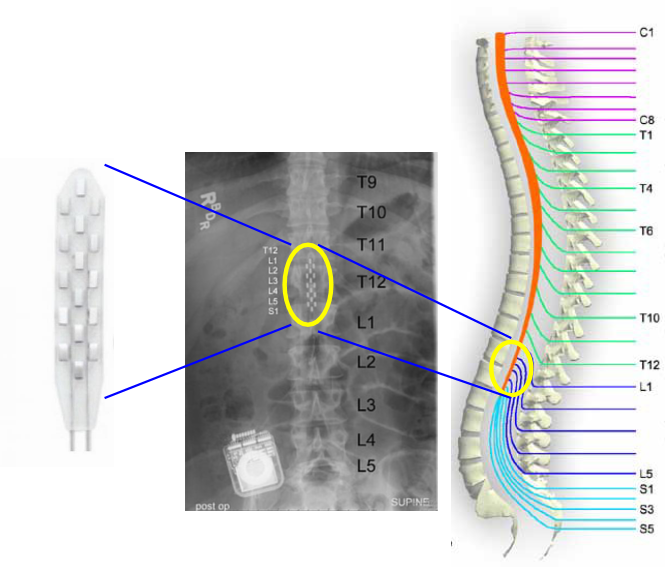
\includegraphics[width=2.5in]{figures/config1.png}
\end{center}
\column{0.45\textwidth}
\begin{center}
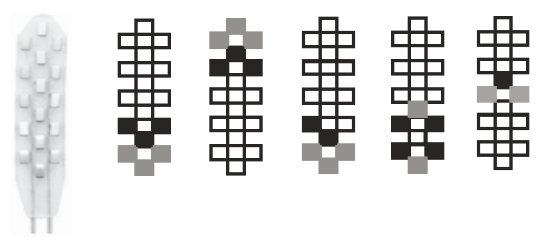
\includegraphics[width=2in]{figures/config2.png}
\begin{itemize}
\item Electrode configurations are represented by points in $\mathbb{R}^4$
\vspace{1em}
\item Data from 351 stimulations (126 distinct configurations)
\end{itemize}
\end{center}
\end{columns}
\end{frame}

\begin{frame}{Experiment 3: Spinal cord therapy}
\begin{columns}[c]
\column{0.55\textwidth}
\begin{center}
\setlength\figurewidth{2.5in}
\setlength\figureheight{1.7in}
\begin{tikzpicture}

\begin{axis}[
title={{\footnotesize stop}},
title style={yshift=-1em},
tick label style={font=\footnotesize},
label style={font=\footnotesize},
width=\figurewidth,
height=\figureheight,
xmin=-0.5, xmax=2.5,
xtick={0, 1, 2},
xticklabels={{\footnotesize\algo}, {\footnotesize\localucb}, {\footnotesize\gpucb}},
%xticklabel style={
%  anchor=base
%},
ymin=0, ymax=100,
ytick={0, 25, 50, 75, 100},
%yticklabel style={rotate=90},
%ylabel=$\%$ of $\Rbeps(S_0)$,
major tick length=2pt,
axis lines*=left]

\addplot [
  ybar,
  bar width=0.4cm,
  cyan!50!black,
  line width=1pt,
  fill=cyan!75!black,
  solid
]
coordinates{
  (0,88.436346)
};

\addplot [
  ybar,
  bar width=0.4cm,
  lime!50!black,
  line width=1pt,
  fill=lime!70!black,
  solid
]
coordinates{
  (1,82.063342)
};

\addplot [
  ybar,
  bar width=0.4cm,
  orange!60!black,
  line width=1pt,
  fill=orange!85!black,
  solid
]
coordinates{
  (2,30.847086)
};

\addplot [
  only marks,
  mark=empty,
  darkgray,
  solid,
  error bars/.cd,
  error bar style={line width=1pt},
  y dir=both,
  y explicit
]
coordinates{
  (0,88.436346) +- (2*4.430386, 2*4.430386)
  (1,82.063342) +- (2*4.201586, 2*4.201586)
  (2,30.847086) +- (2*0.861908, 2*0.861908)
};

\end{axis}

\end{tikzpicture}
\\
\begin{tikzpicture}

\begin{axis}[
title={{\footnotesize non-stop}},
title style={yshift=-1em},
tick label style={font=\footnotesize},
label style={font=\footnotesize},
width=\figurewidth,
height=\figureheight,
xmin=-0.5, xmax=2.5,
xtick={0, 1, 2},
xticklabels={{\footnotesize\algo}, {\footnotesize\localucb}, {\footnotesize\gpucb}},
%xticklabel style={
%  anchor=base
%},
ymin=0, ymax=100,
ytick={0, 25, 50, 75, 100},
%yticklabel style={rotate=90},
%ylabel=$\%$ of $\Rbeps(S_0)$,
major tick length=2pt,
axis lines*=left]

\addplot [
  ybar,
  bar width=0.4cm,
  cyan!50!black,
  line width=1pt,
  fill=cyan!75!black,
  solid
]
coordinates{
  (0,88.118102)
};

\addplot [
  ybar,
  bar width=0.4cm,
  lime!50!black,
  line width=1pt,
  fill=lime!70!black,
  solid
]
coordinates{
  (1,81.768031)
};

\addplot [
  ybar,
  bar width=0.4cm,
  orange!60!black,
  line width=1pt,
  fill=orange!85!black,
  solid
]
coordinates{
  (2,100)
};

\addplot [
  only marks,
  mark=empty,
  darkgray,
  solid,
  error bars/.cd,
  error bar style={line width=1pt},
  y dir=both,
  y explicit
]
coordinates{
  (0,88.118102) +- (2*4.421779,2*4.421779)
  (1,81.768031) +- (2*4.193425,2*4.193425)
  (2,100) +- (2*0,2*0)
};

\end{axis}

\end{tikzpicture}

\end{center}
\column{0.45\textwidth}
\centering
\setlength\figurewidth{2.5in}
\setlength\figureheight{3.6in}
\begin{tikzpicture}

\begin{axis}[
name=plot1,
anchor=above north west,
tick label style={font=\footnotesize},
label style={font=\footnotesize},
title={\footnotesize\algo},
title style={yshift=-1em},
width=\figurewidth,
height=\figureheight/3,
xmin=0.33, xmax=1.02,
xtick={0, 0.2, 0.4, 0.6, 0.8, 1},
ymin=0, ymax=0.21,
ytick=\empty,
yticklabels={,,},
ylabel near ticks,
ylabel shift=-5pt,
major tick length=2pt,
axis lines*=left]

%% \addplot[
%%   color=cyan!75!black,
%%   solid,
%%   line width=1.5pt,
%%   samples=30,domain=0:6
%% ]
\addplot[
  ybar,
  bar width=0.15cm,
  cyan!50!black,
  line width=1pt,
  fill=cyan!75!black,
  solid
]
coordinates{
(0.56, 0.05714285714285714)(0.6, 0.2)(0.64, 0.05714285714285714)(0.6799999999999999, 0.05714285714285714)(0.72, 0.17142857142857143)(0.76, 0.08571428571428572)(0.8, 0.11428571428571428)(0.84, 0.02857142857142857)(0.88, 0.0)(0.92, 0.05714285714285714)(0.96, 0.14285714285714285)(1.0, 0.02857142857142857)
};

\addplot [
  magenta!50!darkgray,
  line width=1pt,
  dashed
]
coordinates{
(0.52512774,0)(0.52512774,60)
};

\addplot [
  mark=diamond*,
  mark size=3,
  only marks,
  cyan!35!black
]
coordinates{
(0.75177565,0)
};

\end{axis}

\begin{axis}[
yshift=-1em,
name=plot2,
at=(plot1.below south west),
anchor=above north west,
tick label style={font=\footnotesize},
label style={font=\footnotesize},
title={\footnotesize\localucb},
title style={yshift=-1em},
width=\figurewidth,
height=\figureheight/3,
xmin=0.33, xmax=1.02,
xtick={0, 0.2, 0.4, 0.6, 0.8, 1},
ymin=0, ymax=0.21,
ytick=\empty,
yticklabels={,,},
ylabel near ticks,
ylabel shift=-5pt,
major tick length=2pt,
axis lines*=left]

%% \addplot[
%%   color=lime!70!black,
%%   solid,
%%   line width=1.5pt,
%%   samples=30,domain=0:6
%% ]
\addplot[
  ybar,
  bar width=0.15cm,
  lime!50!black,
  line width=1pt,
  fill=lime!70!black,
  solid
]
coordinates{
(0.56, 0.034482758620689655)(0.6, 0.13793103448275862)(0.64, 0.13793103448275862)(0.6799999999999999, 0.10344827586206896)(0.72, 0.13793103448275862)(0.76, 0.06896551724137931)(0.8, 0.10344827586206896)(0.84, 0.0)(0.88, 0.06896551724137931)(0.92, 0.10344827586206896)(0.96, 0.10344827586206896)(1.0, 0.0)
};

\addplot [
  magenta!50!darkgray,
  line width=1pt,
  dashed
]
coordinates{
(0.52512774,0)(0.52512774,1)
};

\addplot [
  mark=diamond*,
  mark size=3,
  only marks,
  lime!35!black
]
coordinates{
(0.75088457,0)
};

\end{axis}

\begin{axis}[
yshift=-1em,
name=plot3,
at=(plot2.below south west),
anchor=above north west,
tick label style={font=\footnotesize},
label style={font=\footnotesize},
title={\footnotesize\gpucb},
title style={yshift=-1em},
width=\figurewidth,
height=\figureheight/3,
xmin=0.33, xmax=1.02,
xtick={0, 0.2, 0.4, 0.6, 0.8, 1},
ymin=0, ymax=0.21,
ytick=\empty,
yticklabels={,,},
ylabel near ticks,
ylabel shift=-5pt,
major tick length=2pt,
axis lines*=left]

%% \addplot[
%%   color=orange!85!black,
%%   solid,
%%   line width=1.5pt,
%% ]
\addplot[
  ybar,
  bar width=0.15cm,
  orange!60!black,
  line width=1pt,
  fill=orange!85!black,
  solid
]
coordinates{
(0.36, 0.017857142857142856)(0.4, 0.09821428571428571)(0.44, 0.05357142857142857)(0.48, 0.08035714285714286)(0.52, 0.0625)(0.56, 0.10714285714285714)(0.6, 0.044642857142857144)(0.64, 0.044642857142857144)(0.6799999999999999, 0.05357142857142857)(0.72, 0.03571428571428571)(0.76, 0.05357142857142857)(0.8, 0.05357142857142857)(0.84, 0.044642857142857144)(0.88, 0.03571428571428571)(0.92, 0.15178571428571427)(0.96, 0.044642857142857144)(1.0, 0.017857142857142856)
};

\addplot [
  magenta!50!darkgray,
  line width=1pt,
  dashed
]
coordinates{
(0.52512774,0)(0.52512774,0.7)
};

\addplot [
  mark=diamond*,
  mark size=3,
  only marks,
  orange!35!black
]
coordinates{
(0.66992681,0)
};

\end{axis}

\end{tikzpicture}

\end{columns}
\end{frame}

\begin{frame}{Summary}
\begin{itemize}
\item<1-> We formulated the problem of safe optimization using the concept of reachability
\vspace{2em}
\item<2-> We proposed a simple algorithm with theoretical guarantees
\vspace{2em}
\item<3-> Better sample complexity bound under additional assumptions?
\vspace{2em}
\item<4-> More efficient sampling heuristics?
\end{itemize}
\end{frame}

\end{document}
